\documentclass[11pt,a4paper]{article}
\usepackage[spanish,activeacute]{babel}
\usepackage[utf8]{inputenc}
\usepackage{amsmath}
\usepackage{amsfonts}
\usepackage{amssymb}
\usepackage{graphicx}
\usepackage{color}
\usepackage{listings}
\usepackage{amsthm}
\usepackage{caption}
\usepackage{subcaption}
\usepackage{dsfont}
\usepackage{comment}
\usepackage{enumerate}
\usepackage{mathtools,xparse}
\usepackage{float}
\usepackage{ upgreek }

\usepackage[left=2.50cm, right=2.50cm, top=2.50cm, bottom=2.50cm]{geometry}

\usepackage[]{hyperref}
\hypersetup{
    pdftitle={Apuntes: Aprendizaje Automático},
    pdfauthor={},
    pdfsubject={ },
    pdfkeywords={keyword1, keyword2},
    bookmarksnumbered=true,     
    bookmarksopen=true,         
    bookmarksopenlevel=1,       
    colorlinks=true,   
    linkcolor=black,         
    pdfstartview=Fit,           
    pdfpagemode=UseOutlines,    % this is the option you were lookin for
    pdfpagelayout=TwoPageRight
}

\DeclarePairedDelimiter{\norm}{\lVert}{\rVert}
\NewDocumentCommand{\normL}{ s O{} m }{%
  \IfBooleanTF{#1}{\norm*{#3}}{\norm[#2]{#3}}_{L_2(\Omega)}%
}
\newtheorem{theorem}{Teorema}

\theoremstyle{definition}
\newtheorem{definition}{Definición}[section]


\newtheorem{proposition}{Proposición}[section]


\newtheorem{corolary}{Corolario}[section]


\newtheorem{lema}{Lema}[section]

	\newcommand{\R}{\mathbb{R}}
	\newcommand{\N}{\mathbb{N}}
	\newcommand{\C}{\mathbb{C}}

\title{\huge \bf Apuntes: Aprendizaje Automático}
\author{Mario Muñoz Mesa}
\date{ }

\begin{document}

	\maketitle
	\renewcommand*\contentsname{Índice}	
	\tableofcontents
	
	\newpage
	
	\section{El problema de aprendizaje.}
	\subsection{Introducción}
	La ciencia moderna e ingeniería utilizan modelos basados en principios básicos para describir sistemas físicos, biológicos y sociales; este abordaje comienza con modelos científicos básicos (leyes Newton, teoría Maxwell...), son la base. Bajo este supuesto, los datos experimentales son utilizados para verificar los modelos y estimar algunos parámetros que son difíciles de medir directamente. 
	
	Sin embargo, en muchas aplicaciones los principios subyacentes son desconocidos o los sistemas son demasiado complejos para ser descritos matemáticamente.\\
	Ejemplos, aplicaciones:
	\begin{itemize}
		\item Speech and speaker recognition, Object and Face recognition, Document translation and composition, Recommendation systems, Stock Market Prediction - time series prediction, Automatic Prognosis and Diagnostic in Medicine, Handwritten character recognition, Conducción autónoma
	\end{itemize}
	 En ausencia de modelos clásicos y grandes cantidades de datos, surge el aprendizaje computacional. Hay un cambio de paradigma, de utilizar modelos basados en principios básicos a desarrollar modelos a partir de datos. La habilidad de extraer conocimiento útil oculto en estos datos y actuar con ese conocimiento está siendo cada vez más importante en el mundo competitivo actual.
	 	 Distinguimos dos fases en el funcionamiento de un sistema de aprendizaje:
	 \begin{enumerate}
	 	\item Aprendizaje/estimación (de muestras de entrenamiento)
	 	\item Operación/predicción, cuando las predicciones son hechas para futuro o muestras tests
	 \end{enumerate}
	 Esta descripción asume que las muestras de entrenamiento y test proceden de la misma distribución de probabilidad subyacente (desconocida). Tareas específicas de aprendizaje incluyen:
	 \begin{itemize}
		\item Calisificación (reconocimiento de patrones) o estimación de fronteras de decisión de clase
		\item Regresión: estimación de función desconocida con codominio real
		\item Estimación de la función de densidad de probabilidad (de las muestras)
	 \end{itemize}
	 \begin{definition}[\textbf{Aprendizaje Automático} (definición de Tom Mitchell)]
	 	Un programa de ordenador se dice que aprende de una experiencia $E$ respecto a una clase de tareas $T$ y medida de desempeño $P$, si su desempeño en tareas $T$, medido por $P$, mejora con la experiencia $E$
	 \end{definition}
	 \textit{Ejemplo:} $E$ = ``experiencia de jugar a las damas muchas veces'', $T$ = ``la tarea de jugar a las damas'', $P$ = ``la probabilidad de que el programa gane en el siguiente juego''.
	 
	 \textit{Introducción más intuitiva y resumida:}\\
	 Somos capaces de decir cuándo vemos un árbol, pero ¿somos capaces de definir con precisión un árbol?. No reconocemos un árbol por conocer la definición formal o matemática de árbol, los reconocemos viendo árboles. En otras palabras, aprendemos de datos.
	\begin{figure}[h!]
	\centering
	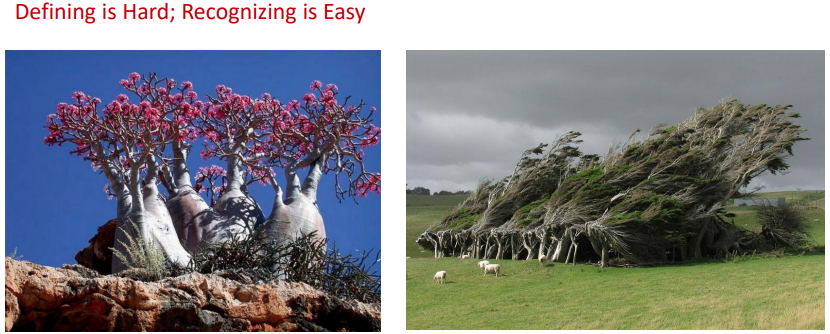
\includegraphics[width=0.55\textwidth]{images/img1_tree}
	\end{figure}
	
	El aprendizaje de datos se utiliza en situaciones donde no tenemos solución analítica, pero tenemos datos que podemos usar para construir una solución empírica.\\
	 
	 

	 
	\section{El problema de aprendizaje (supervisado).}
	
	\subsection{Configuración del problema}
	
	\subsubsection{Componentes del aprendizaje (supervisado)}
		Supongamos un banco que quiere automatizar el proceso de concesión de créditos. Para esto no existe una fórmula explícita que determine cuándo debe concederse el crédito. 
		
		Para cada cliente se tiene información personal relacionada con el problema de concesión de crédito; salario anual, años de residencia, deudas... etc. También se tiene historial de créditos aprobados a clientes y si esa aprobación fue beneficiosa/exitosa.\\
		
		\underline{Generalización y formalización:}
		\begin{itemize}
			\item $f\colon \mathcal{X} \to \mathcal{Y}$, función objetivo desconocida \textit{(fórmula ideal para aprobación de crédito)}
			\item $\mathcal{X}$ conjunto de los posibles datos de entrada del problema \textit{(conjunto donde cada elemento $x\in \mathcal{X}$ contiene la información para tomar la decisión de crédito)}
			\item $\mathcal{Y}$ conjunto de las posibles salidas \textit{(sí o no, a la aprobación de crédito)}
			\item $\mathcal{D}$ muestra de tamaño $N\in \N$ (muestra de entrenamiento), $$\mathcal{D}=\{(x_i,y_i)\in \mathcal{X}\times \mathcal{Y} \ : \ f(x_i)=y_i \quad \forall i\in \{1,...,N\}\}$$ contiene entradas y salidas ya conocidas \textit{(información de clientes previos y la decisión correcta en su caso para el crédito)}
			\item $\mathcal{H}=\{h_\lambda\colon \mathcal{X} \to \mathcal{Y} \ : \ \lambda \in \Lambda\}$ subconjunto de funciones de $\mathcal{X}$ a $\mathcal{Y}$, se llama el conjunto hipótesis. Nota:
			\begin{itemize}
				\item No hay desventaja, porque desde un punto de vista práctico cuando quieres aprender utilizas: función lineal, red neuronal.... (ya utilizas un conjunto de hipótesis). En cualquier caso siempre puedes elegir el conjunto de todas las posibles hipótesis y no hay pérdida de generalidad.
				\item Hay ventajas, nos dirá si podemos aprender, cómo de bien... (se verá más adelante)
			\end{itemize}
			\item $\mathcal{A}$ algoritmo de aprendizaje que en base a $\mathcal{D}$ elige $g\in \mathcal{H}$ que aproxima a $f$, $g\approx f$
		\end{itemize}
		
		\textit{IMPORTANTE.} Premisa\/Hipótesis: las features de $x\in \mathcal{X}$ son independientes; y para la muestra $(x_i,y_i)$ i.i.d. 
		\newpage
	\begin{figure}[h!]
	\centering
	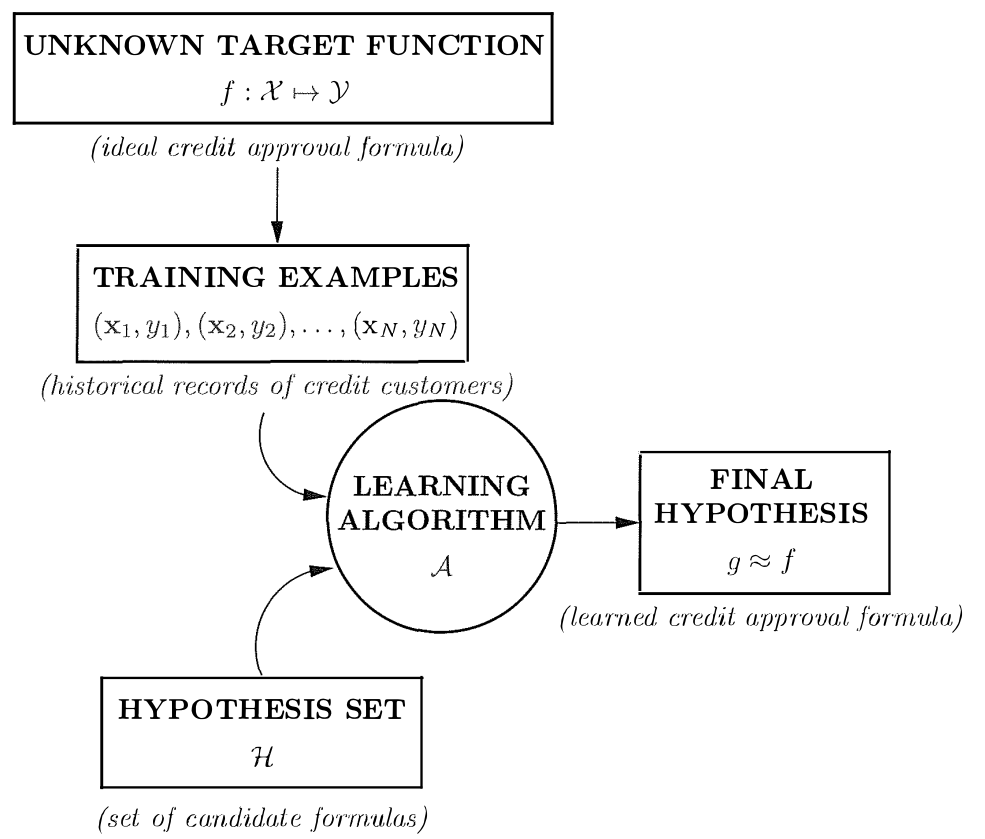
\includegraphics[width=0.75\textwidth]{images/esquema_aprendizaje}
	\end{figure}
	
	Observamos que realmente tenemos,
	\begin{itemize}
		\item $(\Omega, \mathcal{A}, P)$ espacio probabilístico, depende del problema planteado.
		\begin{itemize}
			\item $P$ es desconocida (si no sería un problema de diseño (?)no, si no no hay nada que hacer)
		\end{itemize}
		\item $X^T=(X_1,...,X_n)\colon \Omega \to \R^n$ vector aleatorio, cada $X_i\colon \Omega \to \R$ es una variable aleatoria asociada a una característica, $X_i$ independientes entre sí. Para el problema de aprendizaje se toman $X_i$, $i=1,\ldots n$ independientes entre sí.
		\begin{itemize}
			\item $(\Omega, \mathcal{A}, P) \stackrel{X}{\to} (\R^n, \mathcal{B}^n, P_X)$.  En el esquema anterior $\mathcal{X}=X(\Omega)$	
		\end{itemize}
		\item $Y\colon \Omega \to \R$ variable aleatoria que se desconoce criterio o regla de actuación (se desconoce regla que la define como función), lo que se conoce de ella es $\mathcal{Y}=Y(\Omega)$ (los posibles valores de la misma)
		\begin{itemize}
			\item $(\Omega, \mathcal{A},P) \stackrel{Y}{\to} (\R, \mathcal{B}, P_Y)$
			%\item $P_Y(B)=P_X(Y^{-1}(B))$ (=???!! puede que no mira la condición $i.i.d$ tal vez $Y\colon \Omega \to $)
		\end{itemize}
		\item $(X,Y)\colon (\Omega,\mathcal{A}, P) \to (\R^{n+1},\mathcal{B}^{n+1})$ vector aleatorio
		\item $(X_1,Y_1), ...., (X_N,Y_N)$ una muestra $i.i.d$ (independiente idénticamente distribuida), con $N\in \N$, (aquí cada $X_i$ es un vector aleatorio con $n$ componentes); es la que se utiliza en el entrenamiento del algoritmo. En principio $\mathcal{D}$ es una realización $(x_1,y_1),\ldots, (x_N,y_N)$, (creo que se puede trabajar también con la muestras como va en los resultados)
		\begin{itemize}
		\item $i.i.d.$ es necesario (\hyperref[sec:anexo1]{Anexo 1}), $i.i.d.$ para la función de probabilidad/densidad conjunta $p(x,y)=p(x)p(y|x)$. Independientes si
		$$F_{(X_i,Y_i),(X_j,Y_j)}((x_i,y_i),(x_j,y_j))=F_{(X_i,Y_i)}((x_i,y_i))F_{(X_j,Y_j)}((x_j,y_j))\quad \forall i\neq j, \ \ 1\leq i,j \leq N$$
		\item $p(y|x)$ es la relación que intentamos capturar mediante el algoritmo de aprendizaje
		\item Para el entrenamiento se usa una realización $(x_1,y_1),...,(x_N,y_N)$ de $(X_1,Y_1), ...., (X_N,Y_N)$
		\end{itemize}
		\item $f\colon X \to Y$, $\mathcal{H}=\{h_\lambda \colon X \to Y \ : \ \lambda \in \Lambda\}$
	
	\end{itemize}
	
	\subsubsection{Aprendizaje vs Diseño}
		Mientras el aprendizaje se basa en datos, en abordaje por diseño no usa datos (uno puede deducir $f$ sin necesidad de usar datos).
		
		 Ejemplo: Supongamos que queremos construir un modelo para reconocer monedas por su masa y tamaño $\{(size\_i,mass\_i) \ : \ i=1,...,N\}$
		 
		 \begin{itemize}
		 	\item Diseño: averiguamos el tamaño y masa de cada moneda, así como el número de monedas en circuilación de cada tipo (para conocer la frecuencia). Elaboramos un modelo físico en función de la masa y tamaño,   teniendo en cuenta las variaciones por uso y errores medidos. Finalmente, construimos una distribución de probabilidad en base a $(size, mass)$ que usamos para clasificar.
		 	
		 	\item Aprendizaje: recopilamos datos etiquetados de cada tipo de moneda. El algoritmo de aprendizaje busca una función hipótesis $g$ que clasifique bien los datos. Para clasificar una nueva moneda utilizamos la $g$ aprendida.
		 \end{itemize}
		
		La diferencia principal es el rol que juegan los datos:
		\begin{itemize}
			\item En el abordaje por diseño, el problema está bien especificado y uno puede analíticamente deducir $f$ sin necesidad de ver datos.
			\item En el abordaje por aprendizaje, el problema está mucho menos especificado, y uno necesita datos para precisar $f$.
		\end{itemize}
		Ambos métodos son viables en varias aplicaciones, pero solo el abordaje por diseño es posible in muchas aplicaciones donde la función objetivo es desconocida.
		
		\textit{Nota:} la información disponible es clave para adoptar uno abordaje u otro.
		
	\subsection{Esquema básico de aprendizaje}
	
	\begin{figure}[h!]
	\centering
	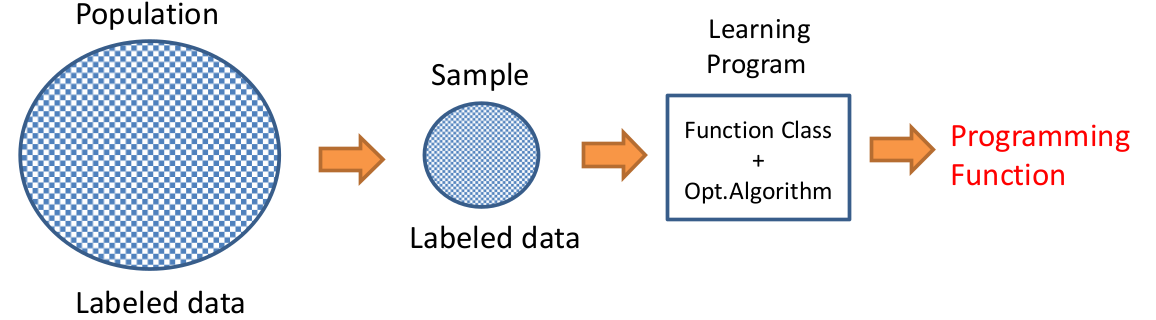
\includegraphics[width=0.75\textwidth]{images/learning_sketch}
	\end{figure}
	Importante: En \textit{Machine Learning} se busca una función final (``programming function'') muy buena que me pueda servir para predecir cualquier elemento nuevo de la población.
	
	La población ($\Omega$), en el caso de clasificar correos en spam y no spam sería: todos los posible correos que me puedan llegar.
	
	¿Cómo elegir muestra y algoritmo para predecir de forma precisa en la población entera? (lo veremos)
	\subsection{Tipos de aprendizaje}
	Hemos visto hasta ahora \textit{Aprendizaje Supervisado}, es el tipo de aprendizaje más estudiado y utilizado pero no es el único.
	\begin{itemize}
		\item Aprendizaje Supervisado: los datos de entrenamiento contienen ejemplos explícitos de cuál debe ser el ``output'' adecuado. 
		\begin{itemize}
			\item Regresión: la salida es un número real (variable continua)
			\begin{itemize}
				\item Predecir la altura de una persona mediante una muestra: peso; (peso, longitud pie); (peso, longitud pie, anchura hombros)... etc
				\item Predecir la temperatura para mañana mediante una base datos de temperaturas previas.
			\end{itemize}
			\item Clasificación: la salida es una etiqueta de clase (variable discreta o categórica)
			\begin{itemize}
				\item Predecir el tiempo para mañana: (soleado, nublado, con viento), (0,1,2)...
				\item Predecir si una imagen contiene una cara: (yes,no), (0,1), (1,-1)...
				\item Predecir si un email es spam o no: (yes,no), (0,1), (1,-1)...
			\end{itemize}
			\item Clasificación probabilística: la salida es un vector de probabilidad sobre cada una de las clases. \\
			\textit{Origen intuitivo:} A veces en problema clasificación hay elementos que están en la frontera entre dos clases, y eso podría generar errores. En este caso ¿por qué no hacer algo intermedio en vez de tomar una clasificación final/definitiva?. Aquí en la salida decimos qué probabilidad creemos que tiene ese elemento de pertenecer a cada una de las clases.
		\end{itemize}
		\item Aprendizaje por Refuerzo: no tenemos ``outputs'' en los datos de entrenamiento. Sin embargo podemos conseguir posibles ``outputs'' junto con medidas de cómo de bueno es cada ``output''.
		\item Aprendizaje no Supervisado: no hay etiquetas, se busca agrupar los datos; muchas veces es la previa para aprendizaje supervisado.\\
		Tres formas de ataque principales, muchos de ellos con representación gráfica. Normalmente técnicas de agrupación y ver qué items caen en cada grupo para ver si realmente son semejantes entre ellos, se distinguen de los items de otro grupo... (entonces sabemos que estamos haciendo algo que podríamos llamar aprendizajes, podemos descubrir algunos patrones o modelos.
		\begin{itemize}
			\item Estructura geométrica: clustering. Ejemplo de grupación por cercanía, se contagian los más cercanos:
			\begin{figure}[htb!]
			\centering
			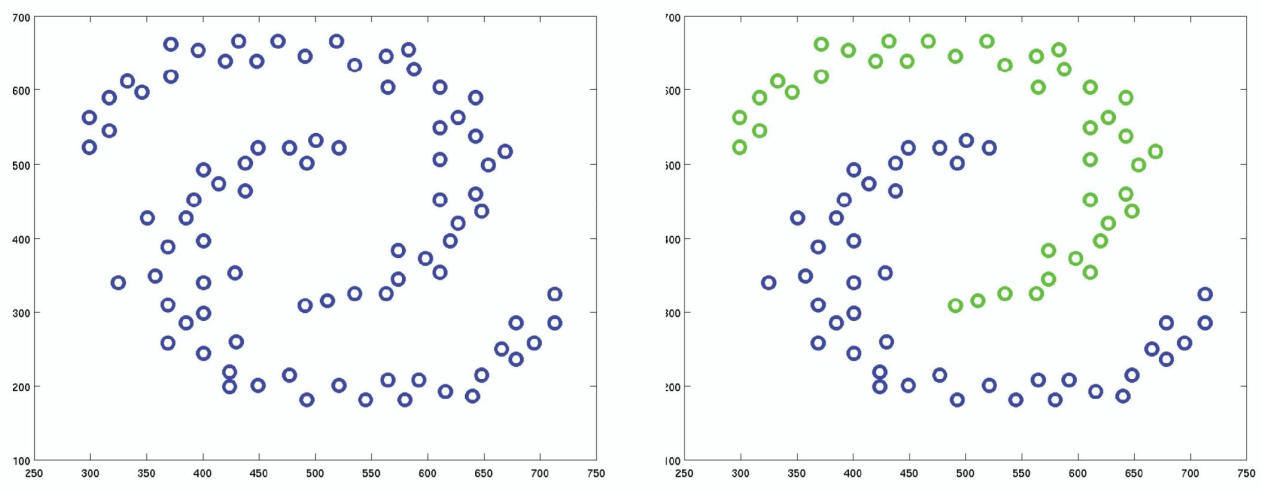
\includegraphics[width=0.65\textwidth]{images/cluster_cercania}
		\end{figure}
		
		
			\item Descubrir dependencias: patrones. De un conjunto de animales y características de los mismo, representamos e intentamos ver dependencias
			\begin{figure}[htb!]
			\centering
			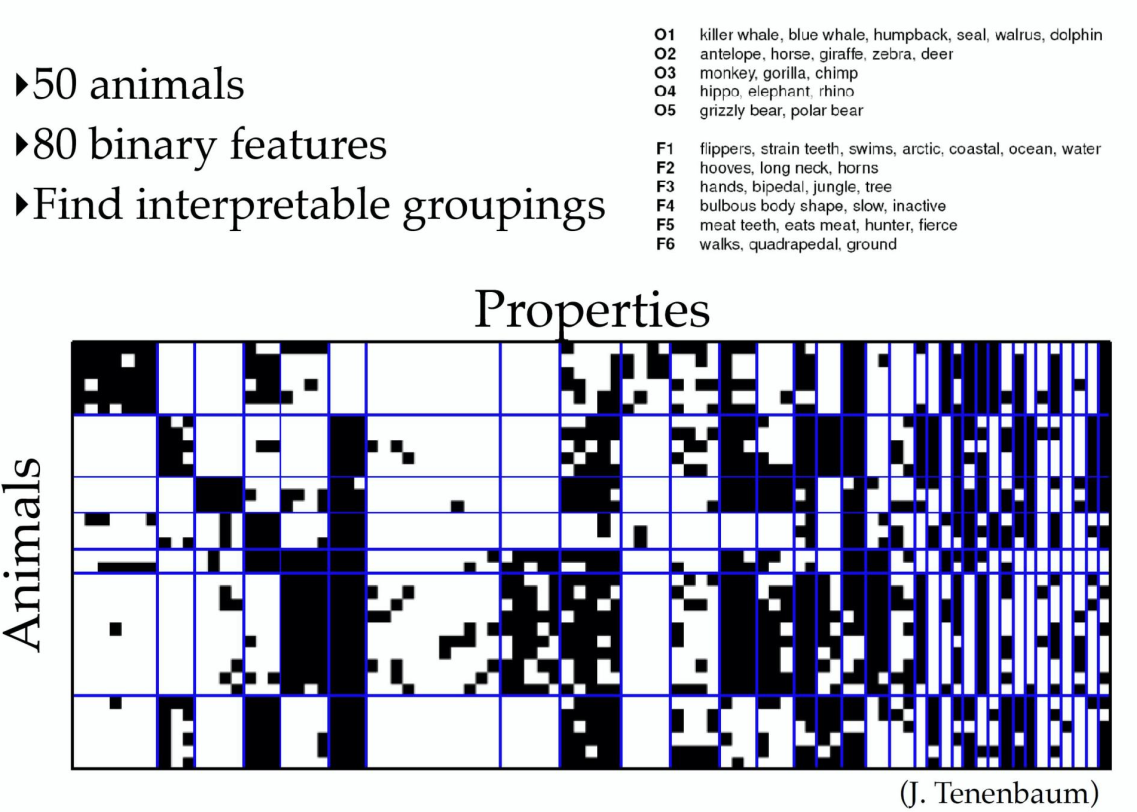
\includegraphics[width=0.45\textwidth]{images/dependencias_animals}
		\end{figure}
		
			\item Reducción dimensionalidad: hechos relevantes. Podríamos tener un vector con muchas dimensiones, para nuestro problema ¿todas esas dimensiones son relevantes? (si no lo son, cada dimensión no relevante añade ruido al problema). Cuando la información tiene las dimensiones realmente necesarias, se aprende bien.
			\begin{figure}[htb!]
			\centering
			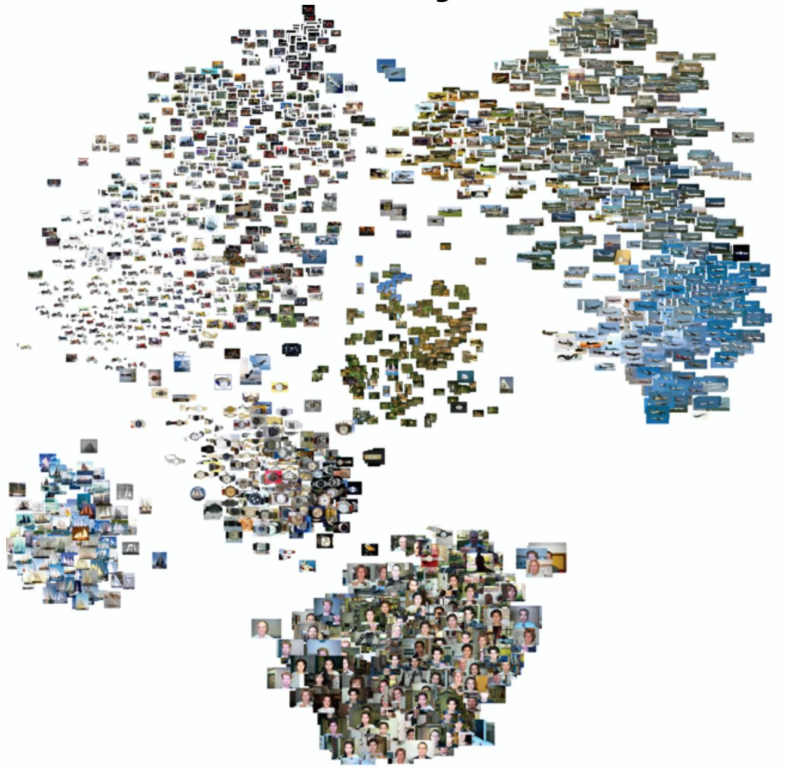
\includegraphics[width=0.45\textwidth]{images/dimensionality}
		\end{figure}
		\end{itemize}
		
	\end{itemize}
	
	\newpage
	
	
	\section{Modelos $\mathcal{H}$-Lineales}
	Esta clase de funciones es una de las más importantes. Si podemos resolver el problema con un modelo lineal, nos encontramos ante una de las mejores situaciones; este es el modelo que más nos explica cómo cada una de las medidas  en el vector de características está influyendo en la solución. Obtener o deducir este tipo de información es muy complicado en modelos no lineales.
	
	Es decir, en modelos lineales tenemos
	
	\begin{itemize}
		\item Baja complejidad de clase de funciones.
		\item Alta capacidad de explicar qué medidas influyen más.
	\end{itemize}
	
	Otros modelos pueden llegar a más precisión en la solución pero a costa de no saber por qué lo hacen ni cómo lo hacen. Salvo los árboles, modelos que ya veremos (son casi tan explicativos como los modelos lineales).
	
	\begin{definition}[\textbf{Clase de funciones $\mathcal{H}$-Lineales}]
	
		Sea $x^T=(x_1,...,x_d)\in \mathcal{X}=X(\Omega)=\R^d$ y $w\in \R^{d+1}$. Se define la clase de los funciones lineales
		$$\mathcal{H}:=\{h_w \colon \R^{d} \to \R \ : \ h_w(x)=w_0+w_1x_1+\ldots + w_dx_d,\ w \in \R^{d+1}\}$$
		si reescribimos $x=(1,x_1,...,x_d)$
		$$\mathcal{H}:=\{h_w\colon \R^{d+1} \to \R \ : \ h_w(x)=w^Tx, \ w \in \R^{d+1}\}$$
		trabajaremos más con esta última expresión.
	\end{definition}
	
	\textit{Notas:}
	\begin{itemize}
	\item Estamos construyendo un modelo en que cada medida tiene un peso para la aproximación final.
	\item Utilizar modelo $\mathcal{H}$-Lineal es siempre opción de primera línea.
	\end{itemize}
	
	Estos modelos se utilizarán para 
	\begin{itemize}
		\item Regresión
		\item Clasificación
		\item Estimación probabilística
	\end{itemize}
	Por ejemplo, en nuestro ejemplo del crédito podemos hacer regresión (dollar amount) o clasificación (yes/no).
	
	\subsection{Regresión Lineal}
	En regresión para calcular el error cometido al aproximar $f$ por $h_w\in \mathcal{H}$ se utiliza el error cuadrático
	$$Error(x)=(h_w(x)-f(x))^2$$
	
	\begin{definition}[\textbf{Error en la muestra (Regresión)}]
	Para una muestra, $(x_1,y_1),\ldots,(x_N,y_N)$ de tamaño $N$, se define el error en la muestra para una función $h_w\in \mathcal{H}$ 
		$$E_{in} (h_w):=\frac{1}{N}\sum_{i=1}^N(h_w(x_i)-y_i)^2$$
	es decir, la media del error cuadrático en cada uno de los elementos de la muestra. Equivalentemente
	$$E_{in} (w):=\frac{1}{N}\sum_{i=1}^N(w^Tx_i-y_i)^2$$
	\end{definition}
	
	\begin{definition}[\textbf{Error fuera de la muestra}]
	Se define el error fuera de la muestra para $h_w \in \mathcal{H}$ como
	$$E_{out}(h_w)=E_{(X,Y)} \left[(h_w(X)-Y)^2\right]$$
	\end{definition}
	
	Nuestro objetivo es encontrar $\hat h_w \in \mathcal{H}$  que minimice $E_{out}$ (la idea es predecir para valores fuera de la muestra). Buscamos $\hat h_w \in \mathcal{H}$ tal que
	$$E_{out}(\hat h_w)=\min_{h_w\in \mathcal{H}} E_{out} (h_w)$$
	
	\begin{itemize}
	\item	En el caso de Regresión Lineal, la $h_w$ que mejor aproxima dentro de la muestra será la que mejor aproxime fuera de la muestra.
	\item Utilizar no solo los valores de la muestra si no también sus cuadrados podría dar un valor más pequeño de $E_{in}$. Pero entonces la $h$ obtenida añadiendo estos nuevos valores al cuadrado es mejor que la $h$ sin estos? $\Rightarrow$ no necesariamente.
	\end{itemize}
	
	Para encontrar $\hat h$ usaremos el principio o criterio (de aprendizaje) ERM (Empirical Risk Minimization), buscamos el $w_{lin}\in \R^{d+1}$ tal que
	$$E_{in}(w_{lin})=\min_{w\in \R^{d+1}} E_{in}(w)$$
	el vector de pesos que minimice el error en la muestra; a partir de ahora nos referiremos a éste con $w_{lin}$\\
	
	El \textit{Ordinary Least Square model (OLS)}, así se le denomina al método consistente en minimizar el error cuadrático medio, solo asume error en la variable dependiente
	\begin{itemize}
		\item Esta hipótesis no es válida en todos los casos.
		\item Pero es una buena aproximación en muchos casos.
	\end{itemize}
	
	\begin{theorem}[\textbf{Teorema de Gauss-Markov}]
	Supongamos que $Y\colon \Omega \to \R$ depende de $X\colon \Omega \to \R^n$ vector aleatorio mediante
	$$Y=X^T \beta + \varepsilon$$
	donde 
	\begin{itemize}
	\item $\varepsilon$=``error o ruido aleatorio'' es una variable aleatoria que recoge todos los factores de la realidad no controlables u observables (se asocian al azar).
	\item $\beta \in \R^n$, $X\colon \Omega \to \R^n$
	\end{itemize}
	Al tomar una muestra $(X_1,Y_1),...,(X_N,Y_N)$ con $X_i\colon \Omega \to \R^n$ tenemos
	$$Y_i=X_i^T \beta + \varepsilon_i \quad \quad i=1,...,N$$
	Supongamos que
	\begin{itemize}
		\item $E[\varepsilon_i]=0$ (errores fluctuan alrededor del 0; que es lo normal cuando se toman medidas, a veces un poco por arriba otra por abajo, pero no hay un sesgo; el aparato de medida no suma nada)
		\item $Cov(\varepsilon_i,\varepsilon_j)=0$, $i\neq j$ (ruidos incorrelados, que no haya ninguna dependencia (ni tendencia) entre una medida y otra.)
		\item $Var(\varepsilon_i^2)=\sigma^2 < \infty$ (que lo que fluctúa el error o ruido esté acotado)
	\end{itemize}
	Entonces \textit{OLS} proporciona el estimador, $\hat \beta$ de mínima varianza (con una muestra yo obtengo un estimador, con otra muestra otro, pero las diferencias entre ellos tienen que ser pequeñas; porque ese estimador varía lo mínimo posible) tal que $E[\hat \beta_i]=\beta_i$ (insesgado) (si calculáramos la media de las estimaciones de calcular distintas muestras, la media de todas, sería la verdadera solución). Es decir $\hat \beta$ es el UMVUE para $\beta$.
	\end{theorem}
	
	Ilustración de regresión lineal:
	\begin{figure}[h!]
	\centering
	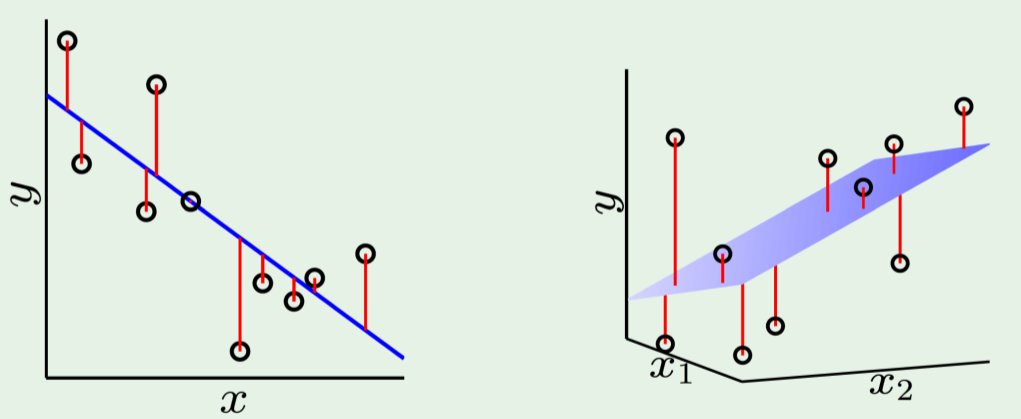
\includegraphics[width=0.75\textwidth]{images/recta_y_plano}
	\caption{Recta y plano de regresión.\\ Cuando $x$ tiene más de 2 variables se habla de hiperplano}
	\end{figure}
	
	En lo que sigue, se asumen las hipótesis del \textit{Teorema de Gauss-Markov}, para aplicar \textit{OLS}.
	
	\subsubsection{Un algoritmo de regresión lineal}
	
	\underline{Expresión matricial para $E_{in}$}
	$$E_{in}(w)=\frac{1}{N} \sum_{i=1}^N (w^Tx_i -y_i)^2=\frac{1}{N}\norm{Xw-y}^2$$
	donde
	$$
	X=\begin{matrix}
	& \left(\begin{matrix}
	- x_1^T - \\
	- x_2^T - \\
	...  \\
	- x_N^T - \\
	\end{matrix}\right)
	\end{matrix}
		\quad \quad 
	y=\begin{matrix}
	& \left(\begin{matrix}
	y_1 \\
	y_2 \\
	...  \\
	y_N  \\
	\end{matrix}\right)
	\end{matrix}
	$$
	
		\textit{Comentario:} Dado $x$ vector columna, $\frac{d}{dx} f \equiv \nabla f$ cuando $f\colon \R^n \to \R$. Es decir, cuando derivamos una expresión en $\R$ respecto a un vector columna las derivadas parciales se van realizando en columna, obteniendo vector columna. Cuando $x$, $y$ vectores columna y $y=y(x)$, entonces $\frac{d}{dx} y$ es la jacobiana traspuesta (en una misma columna va cambiando la variable de derivación conforme bajas filas)

	\begin{proposition}[\textbf{Cálculo vectorial y matricial}]
	Denotamos con mayúsculas matrices y con minúsculas vectores columna
	\begin{itemize}
		\item $a^Tb=b^Ta$
		\item $y^TXw=w^TX^Ty=(Xw)^Ty$ (ver el primer producto como un vector y ver que puedo conmutar con traspuesta el producto de vector fila con columna)
		\item $\frac{d}{dx}(x^TAx)=(A^T+A)x$
		\item $\frac{d}{dx} (x^Ta)=a$, $\frac{d}{dx} (a^Tx)=a$, $\frac{d}{dx^T} (a^Tx)=a^T$
		\item $\frac{d}{dx} (Ax)=A^T$%$\frac{d}{dx} (Ax)=A$
		\item $\frac{d}{dx} (x^TA)=A$%$\frac{d}{dx} (x^TA)=A^T$
	\end{itemize}
	\end{proposition}
	
	\underline{Minimizando $E_{in}$}
	\begin{proposition}[\textbf{Cálculo de $w_{lin}$}]
	$$E_{in}(w)=\frac{1}{N}\norm{Xw-y}^2$$
	para minimizar igualamos gradiente a 0
	$$\nabla E_{in}(w)=\frac{2}{N} X^T (Xw-y)=0$$
	y queda
	$$X^TXw= X^Ty$$
	que se reescribe como
	$$w=X^\dagger y \quad \text{ donde } \quad X^\dagger :=(X^TX)^{-1}X^T \ \ \text{ (pseudo-inversa de } X\text{)}$$
	$\Rightarrow w_{lin}=(X^TX)^{-1}X^Ty$
	\begin{proof}
	$$\norm{Xw-y}^2=(Xw-y)^T(Xw-y)=(Xw)^TXw-y^TXw-(Xw)^Ty+y^Ty=$$
	$$=w^TX^TXw-2w^TX^Ty+y^Ty$$
	$\Rightarrow \frac{d}{dw}=2X^TXw-2X^Ty$ $\Rightarrow w_{lin}=(X^TX)^{-1}X^Ty$
	\end{proof}
	
	\end{proposition}
	
	Es decir, hemos conseguido una expresión cerrada, no hay que iterar. Esto es siempre que, con los datos de la muestra, pueda calcular $(X^TX)^{-1}X^T$\\
	
	\textit{Problema:} no escala bien, muchos datos pueden resultar en una matriz demasiado grande.\\
	
	\begin{proposition}[\textbf{¿Cuándo podemos calcular $(X^TX)^{-1}$?}] $\ $
	\begin{enumerate}
	\item Dada una matriz $m\times n$ real, el \textit{Singular Value Decomposition (SVD)} nos asegura poder expresar $X=UDV^T$ con $D$ matriz diagonal con los valores singulares de $X$ como elementos de la diagonal, y $U,V$ matrices ortogonales ($V^T=V^{-1}$, $U^T=U^{-1}$)
	
	\item Por lo que $X^TX=VDU^TUDV^T=VDDV^T$. 
	\item Y por tanto $(X^TX)^{-1}=V^{-T}D^\dagger V^{-1}=VD^\dagger V^T$ siempre puede ser calculado. Aquí $D^\dagger$ denota (no es pseudo-inversa), si $D$ tiene $e_1,\ldots,e_d$ como elementos de la diagonal, la matriz que en su diagonal tiene $\frac{1}{e_i^2}$ como elementos o $0$ si $e_i=0$
	\item 
	\begin{itemize}
		\item Si rango$(X^TX)=d$ $\Rightarrow$ solo existe una solución
		\item Si rango$(X^TX)<d$ $\Rightarrow$ existen infinitas soluciones
	\end{itemize}
	\end{enumerate}
	\end{proposition}
	
	Por lo que siempre podemos calcular $(X^TX)^{-1}$, y siempre podemos utilizar este algoritmo por Pseudoinversa.
	
	En resumen, el algoritmo es
		\begin{figure}[h!]
	\centering
	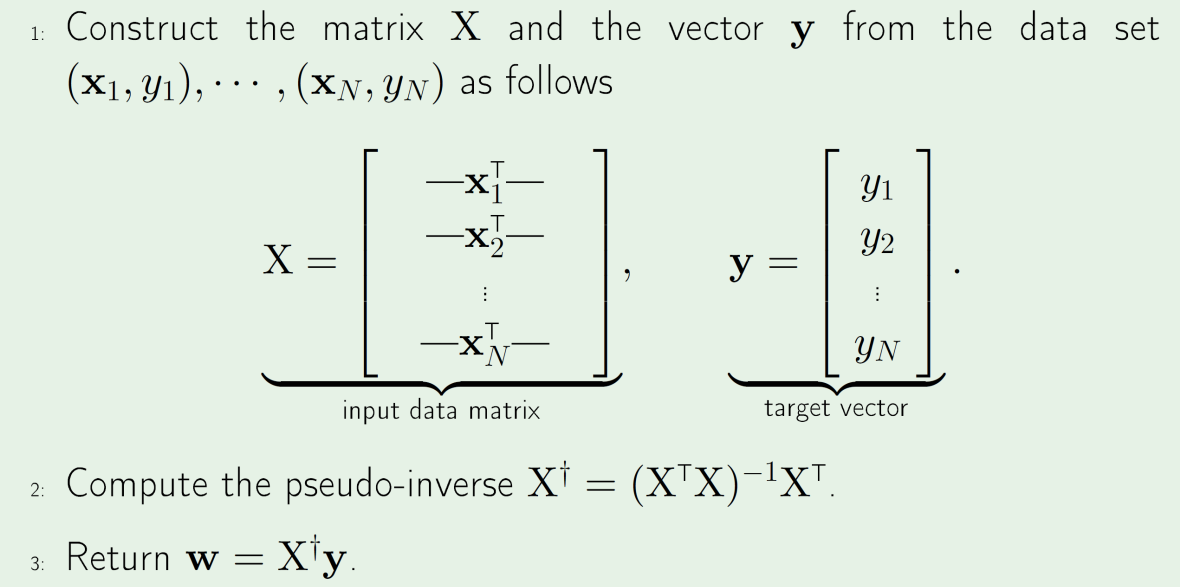
\includegraphics[width=0.75\textwidth]{images/algo_regre_b}
	\caption{Esquema del algoritmo de regresión}
	\end{figure}

	Siempre podemos calcularlo.\\
		\textit{Problema:} no escala bien, muchos datos pueden resultar en una matriz demasiado grande.\\	
		
	\begin{definition}[\textbf{Hat Matrix}]
		Recordamos que la matriz $X$, asociada a la muestra de tamaño $N$ y vector de características de tamaño $d+1$, tiene dimensión $N\times (d+1)$. Y que una forma de obtener un vector de  aproximaciones, $\hat y$, de las clases para cada uno de los datos de la muestra sería
		$$\hat y=X w_{lin}=X(X^TX)^{-1}X^Ty=\hat H y$$
		Llamamos \textit{Hat Matrix}, $\hat H$, a $\hat H=X(X^TX)^{-1}X^T$
		
	\end{definition}
	
	\textit{Observación:} $\hat H$ actúa como función de $y$ a $\hat y$
	
	\begin{proposition}[\textbf{Propiedades de $\hat H$}] $\ $
	\begin{itemize}
		\item $\hat H$ es idempotente, $\hat H^2=\hat H$. \\Si proyecto $y$ con $\hat H$ obtengo $\hat y$, volver a proyectar sobre $\hat y$ me vuelve a dar $\hat y$.
		\item traza($\hat H$)$=d+1$\\
		Nos da un indicador del verdadero número efectivo de valores en el vector que son independientes. Nos ayuda a identificar la dimensionalidad efectiva del problema. Dimensiones que aportan, valores del vector que están diciendo algo nuevo (no que repiten lo que ya nos dicen otros valores). Nos ayuda a identificar la dimensionalidad efectiva de nuestro problema. \textit{Nota:} esto es porque desde el principio estamos trabajando con la hipótesis de que tomamos $d$ características (var. aleatorias) independientes en el vector de características.\\
		
		Cuando uno extrae los valores de los ítems, uno no sabe si son o no independientes. Uno los extrae porque piensa que son relevantes para el problema. El análisis de la traza de $\hat H$ nos dice el número efectivo de valores que son independientes. Ayuda a identificar la dimensionalidad efectiva del problema.
	\end{itemize}
	
	\end{proposition}
	\textit{Nota:} las propiedades de $\hat H$ son relevantes para el análisis de $E_{out}$ y $E_{in}$
	
	\textit{Nota:} la siguiente proposición solo se da en \textit{Regresión Lineal}
	\begin{proposition}
	Para regresión lineal podemos encontrar la fórmula exacta
	$$E_{out}(w_{lin})=E_{in}(w_{lin})+\underbrace{\mathcal{O}\left(\frac{d}{N}\right)}_{\text{notación O-grande}}$$
	es decir, $E_{out}(w_{lin})=E_{in}(w_{lin})$ cuando $N\to \infty$, ($d$ es una constante que ya se especificará)
	\end{proposition}
	Es decir, aumentando el tamaño de la muestra puedo ir minimizando el error fuera de la muestra, que es lo que verdaderamente queremos.
	
	\subsubsection{Gradiente Descendente}
	Este algoritmo no está enfocado a ``despejar'' $w$ óptima. Se busca aproximar $w$ paso a paso, iterativamente, lo mejor posible.
	
	Gradiente Descendente es una técnica general para minimizar funciones 2 veces derivables, como $E_{in}(w)$. Una analogía ilustrativa es una bola rodando por una superficie con colinas. Si la bola se emplaza en la colina, esta desciende hasta encontrar un valle (mínimo local). Igual ocurre con $E_{in}(w)$, que se puede representar como una superficie de altas dimensiones.
	
	 En el paso 0, empezamos en punto $w_0$.
	
	\textit{Nota:}  en el caso de $E_{in}(w)$ solo tiene un bajada por ser convexa, no hay mínimo locales solo uno global (el estudio se hará en general).
	
	Tenemos que determinar cómo bajar por $E_{in}$ mediante el paso más profundo. Supongamos que tomamos un paso de tamaño $\eta$ en la dirección de un vector unitario $\hat v$, $\norm{\hat v}=1$. Los nuevos pesos serán $w_0+\eta \hat v$. Queremos, dado $w_0$, encontrar $\hat v$ tal que $$E_{in}(w_0+\eta \hat v)<E_{in}(w_0)$$
Se toma $\eta$ pequeño, $\eta \approx 0$. Aplicaremos desarrollo de Taylor de 1er orden en la siguiente expresión
	$$\Delta E_{in}=E_{in}(w_0+\eta \hat v) - E_{in}(w_0)\stackrel{Taylor}{=} \eta \nabla E_{in}(w_0)^T\hat v + \underbrace{\mathcal{O}(\eta ^2)}_{\text{O-grande}} \geq  \eta \nabla E_{in}(w_0)^T\hat v  =$$ $$ \stackrel{(*)}{=}-\eta \norm{\nabla E_{in}(w_0)}$$
	(*) En la última igualdad tenemos el producto del vector fila $\eta \nabla E_{in}(w_0)^T$ (que es evaluar $w_0$ en el gradiente de $E_{in}$ como fila), y por otro lado el vector que yo quisiera elegir $\hat v$. Para que este producto escalar sea máximo $\hat v$ debe tener misma dirección y sentido que $\eta \nabla E_{in}(w_0)^T$, así el coseno del ángulo que forman será 1. Pero como lo que nosotros buscamos es minimizar, tomaremos sentido opuesto para que el producto sea negativo (notar de nuevo que buscamos $E_{in}(w_0+\eta \hat v)<E_{in}(w_0)$). Entonces $\eta \nabla E_{in}(w_0)^T$ y $\hat v$ coinciden en la misma dirección pero con sentidos opuestos, es decir, $\hat v$ tiene la dirección y sentido de $-\nabla E_{in}(w_0)$. Finalmente, basta hacer el producto escalar de $\eta \nabla E_{in}(w_0)^T$ y $\hat v$  para ver la igualdad $$\eta \nabla E_{in}(w_0)^T \hat v\stackrel{(*)}{=} \eta \norm{\nabla E_{in}(w_0)^T} \norm{\hat v} \cos(\pi)=-\eta \norm{\nabla E_{in}(w_0)} \Leftrightarrow$$
	$$\Leftrightarrow \nabla E_{in}(w_0)^T \hat v= -\norm{\nabla E_{in}(w_0)} \Leftrightarrow \frac{\nabla E_{in}(w_0)^T \hat v}{\norm{\nabla E_{in}(w_0)}}= -1 \Leftrightarrow \hat v=-\frac{\nabla E_{in}(w_0)}{\norm{\nabla E_{in}(w_0)}}$$
	Por tanto
	$$\hat v=-\frac{\nabla E_{in}(w_0)}{\norm{\nabla E_{in}(w_0)}}\quad \quad \text{ (gradiente negativo)}$$
	
	¿Cómo elegir $\eta$? (decreciendo conforme nos acercamos a óptimo)
		\begin{figure}[h!]
	\centering
	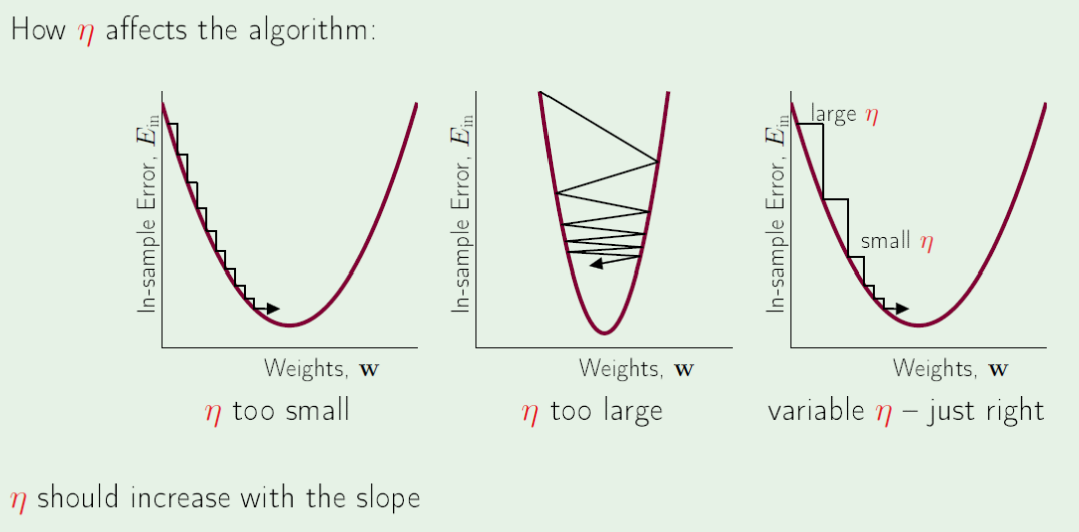
\includegraphics[width=0.75\textwidth]{images/tasa_apren}
	\caption{Cómo elegir $\eta$}
	\end{figure}
	
	Lo ideal sería hacer $\eta$ pequeña conforme nos acercamos al óptimo para evitar así conducta oscilatoria. Esto sería lo ideal. En la práctica tenemos una superficie desconocida y no sabemos si estamos cerca o lejos del óptimo. Hay mucho de experimentación o de arte en la elección de los valores de $\eta$. Muchas veces se toma una fórmula general para ir eligiendo $\eta$, por ejemplo: inversamente proporcional al número de pasos. Tampoco sabes donde has iniciado el $w_0$, no será una regla útil en todos lo casos.\\
	
	\underline{Proceder}\\
	Se empieza con un valor $w_0$, $w=w_0$, y se actualiza el valor repetidamente
	$$w_j:=w_j-\eta \frac{d}{dw_j}E_{in}(w) \quad j \in \{0,...,d\}, \quad \text{ abreviadamente } \quad w:=w-\eta \nabla E_{in}(w)$$
	con
	$$\frac{d}{dw_j}E_{in}(w)=\frac{d}{dw_j}\frac{1}{N}\sum_{n=1}^N (w^Tx_n-y_n)^2=\frac{2}{N}\sum_{n=1}^N x_{nj}(w^Tx_n-y_n)=\frac{2}{N}\sum_{n=1}^N x_{nj}(h(x_n)-y_n)$$
	\textit{Nota:} conforme se va actualizando $w$, $w^Tx_n-y_n$ (que va midiendo el error de aproximación a valor etiqueta) va disminuyendo. El cómo cambia $w_j$ en cada paso tiene que ver en cómo es de buena la aproximación, si estuviésemos en el óptimo tendríamos $w^Tx_n=y_n$ $\forall n \in \{1,\ldots,N\}$ y el gradiente valdría 0, $\frac{d}{dw_j}E_{in}(w) = 0 \ \ \forall j \in \{1,\ldots,d+1\}$
	
	\begin{itemize}
		\item Cada $(x_n,y_n)$ contribuye a la actualización por una catidad proporcional al error de predicción.
		\item En este caso todos los puntos se usan para calcular el gradiente (\textit{Bach Gradient Descent})
		\item Se ha visto que el uso de todos los puntos dificultan encontrar un buen óptimo.
	\end{itemize}
	
	%También se puede escribir abreviadamente
	%$$w:=w-\eta \nabla E_{in}(w)$$
	
		\begin{figure}[htb!]
	\centering
	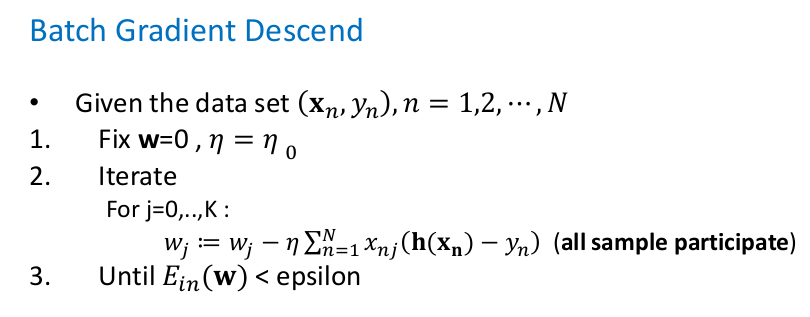
\includegraphics[width=0.75\textwidth]{images/batch_GD}
	\caption{Esquema Batch Gradient Descend}
	\end{figure}
	
	\textit{Observaciones:}
	\begin{itemize}
	\item	El criterio de parada puede ser $E_{in} < \varepsilon$ o un número de iteraciones.
	\item Problema métodos iterativos: tienen un punto inicial y no tienes garantía de llegar al óptimo global (salvo que sepas que la función que minizas sea convexa, como es el caso de $E_{in}$).
	\end{itemize}
	
	\subsubsection{Gradiente Descendente Estocástico (SGD)}
	Este es el que vamos a usar. Este método solo utiliza un parte de la muestra (se ha visto que esto mejora sustancialmente). Utilizar minibatchs (pequeñas submuestras de la muestra) y utilizarlos para el cálculo de gradiente se ha visto que mejoran los óptimos. Por ejemplo de una muestra de 1000 utilizar 30, 40 o 70. 
	
	De una muestra de tamaño $N$ se toma un $M << N$ (mucho más pequeño)
	
	$$\frac{d}{dw_j}E_{in}(w)=\frac{2}{M}\sum_{n=1}^M x_{nj}(h(x_n)-y_n)$$
	
	\begin{itemize}
		\item Mayor variabilidad en la estimación del gradiente (menos ejemplos en la media)
		\item Muy rápido de computar
		\item En funciones no convexas hay evidencia empírica de obtener un buen óptimo local
	\end{itemize}

	Se toma una tasa de aprendizaje $\eta$, un punto inicial $w=w_0\in \text{Dominio}(E_{in})$. Se divide la muestra en una secuencia de minibatchs aleatorios. Iteramos los minibatchs y en base a cada minibatch, $minibatch \in Minibatchs$, se actualiza el valor de $w$
	$$w:=w-\eta \nabla E_{in}^{minibatch}(w)$$
	repetimos esta división en minibatchs y los cálculos de $w$ por cada $minibatch \in Minibatchs$ \iffalse esta toma de minibatch y cálculo de $w$ en función del minibatch\fi hasta una condición de parada, ya sea por iteraciones o por encontrar un valor suficientemente pequeño para $E_{in}$\\
	
	\begin{figure}[H]
	\centering
	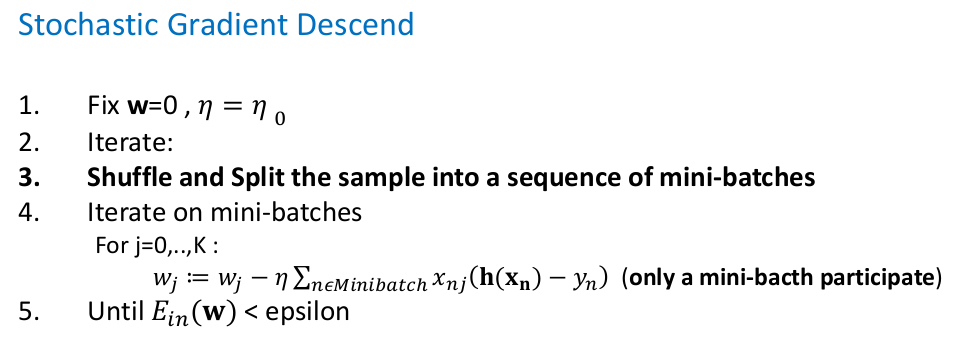
\includegraphics[width=0.75\textwidth]{images/Sto_GD}
	\caption{Esquema Stochastic Gradient Descend}
	\end{figure}	
	
	Si iteras por punto 4 y terminas, y en punto 5 no se cumple; entonces repetir empezando por punto 3.

	\textit{Observaciones:}
	\begin{itemize}
	\item	El criterio de parada puede ser $E_{in} < epsilon$ o un número de iteraciones.
	\item Problema métodos iterativos: tienen un punto inicial y no tienes garantía de llegar al óptimo global (salvo que sepas que la función que minizas sea convexa, como es el caso de $E_{in}$).
	\end{itemize}
	
	\subsubsection{Método de Newton (cura para la oscilación)}
	¿Cuándo utilizarlo? Cuando estemos muy cerca de óptimo verdadero porque hayamos avanzado con algún método, \textit{Gradiente Descendente} por ejemplo, y vemos que los valores de las derivadas ya no son valores muy grandes. En ese caso estamos cerca del óptimo local que vamos a conseguir. Podríamos seguir iterando..., la alternativa que ofrece este método es hacer una aproximación al óptimo suponiendo una superficie en paraboloide (buscar óptimo del paraboloide y suponer que ese óptimo es nuestro óptimo).\\
	
	A diferencia de \textit{Gradiente Descendente}, utilizaremos desarrollo Taylor de 2do orden (2do orden nos aporta aproximación de la curvatura en un entorno). Denotamos por $H_{E_{in}}$ a la matriz \textit{Hessiana} de $E_{in}$
	\begin{itemize}
	\item Nueva regla de actualización para $w$ basada en las derivadas de segundo orden. Ilustramos para una función genérica $f\colon \R^2 \to \R$ con $f\in \mathcal{C}^2(\R^2)$, (utilizaremos la matriz Hessiana  $H_f$)
	$$f(x+\Delta x,y + \Delta y)\stackrel{Taylor}{\approx}$$
	$$\stackrel{Taylor}{\approx} f(x,y)+\frac{df}{dx}\Delta x+ \frac{df}{dy}\Delta y + \frac{1}{2}\left(\frac{d^2f}{dx^2} \Delta x^2 + \frac{d^2f}{dy^2} \Delta y^2 + \frac{d^2 f}{dydx} \Delta x \Delta y + \frac{d^2 f}{dxdy} \Delta x \Delta y\right)=$$
	$$=f(x,y)+\nabla f(x,y)^T \begin{pmatrix}\Delta x\\ \Delta y \end{pmatrix} + (\Delta x \ \Delta y) \underbrace{\begin{matrix}
	 \left(\begin{matrix}
	\frac{\partial}{\partial x^2} f(x,y) & \frac{\partial}{\partial y \partial x} f(x,y) \\
	\frac{\partial}{\partial x \partial y} f(x,y) & \frac{\partial}{\partial y^2} f(x,y)\\
	\end{matrix}\right)
	\end{matrix}}_{H_f}  
	\begin{pmatrix}\Delta x\\ \Delta y \end{pmatrix}$$	
	\item Supongamos que ya estamos en un $w_0$ bueno (está cerca del óptimo). Vamos a ver si se puede calcular un incremento $\Delta w$ para que $w_0+ \Delta w$ sea el valor que nos da el óptimo
	$$g(\Delta w)=E_{in}(w_0+\Delta w) \stackrel{Taylor}{\approx} \underbrace{E_{in}(w_0)}_{f(x,y)}+\underbrace{\Delta w^T\nabla E_{in}(w_0)}_{\frac{df}{dx}\Delta x+ \frac{df}{dy}\Delta y }+\underbrace{\frac{1}{2} \Delta w^T \nabla ^2 E_{in} (w_0)\Delta w}_{\frac{1}{2}\left(\frac{d^2f}{dx^2} \Delta x^2 + \frac{d^2f}{dy^2} \Delta y^2 + \frac{d^2 f}{dydx} \Delta x \Delta y + \frac{d^2 f}{dxdy} \Delta x \Delta y\right)}$$
	Ahora imponemos $\frac{\partial g(\Delta w)}{\partial\Delta w}=0$ (queremos llegar al mínimo, notar que se impondrá sobre la aproximación), y como 
	$$\frac{\partial}{\partial \Delta w} \left( \frac{1}{2} \Delta w^T \nabla ^2 E_{in} (w_0)\Delta w \right) = \frac{1}{2} \underbrace{\left( \nabla ^2 E_{in}(w_0) + (\nabla ^2 
E_{in}(w_0))^T\right)}_{ 2 \nabla ^2 E_{in}(w_0) } \Delta w  $$  
	(en las últimas llaves se usa la conmutatividad de derivadas parciales por Teorema de Schwartz), queda
	$$\nabla E_{in}(w_0)+\underbrace{\nabla^2 E_{in}(w_0)}_{H_{E_{in}}(w_0)} \Delta w=0$$
si $H_{E_{in}}(w_0)$ es definida positiva entonces la evaluación de $w_0 + \Delta w$, en la aproximación cuadrática (la que nos da el desarrollo de Taylor de 2do orden), da un mínimo local en la aproximación, y podemos determinar el paso necesario, $\Delta w$, para obtener el valor, $w_0+\Delta w$, que minimiza a la aproximación
	$$\Delta w=-H_{E_{in}}(w_0)^{-1} \nabla E_{in} (w_0)$$
	Si partíamos de un $w_0$ suficientemente próximo de un punto que da mínimo de $E_{in}$, nos dará una buena aproximación del punto que da ese mínimo de $E_{in}$ (esto es importante, puede ayudar a curar la oscilación)
	
	Después se puede tomar $w_0=w_0 +\Delta w$ y repetir el proceso. Es un método iterativo.
	\end{itemize}
	Notas:
	
	\begin{itemize}
		\item No se determina $\eta$ como en el método \textit{Gradiente Descendente}, este método directamente determina la dirección y el tamaño del paso.
	
		\item Este método debe de utilizarse cuando se está cerca del óptimo (la información sobre la curvatura en $E_{in}(w_0)$ dada por $H_{E_{in}}(w_0)$ es local, si no estamos lo suficientemente próximos podría ser  $H_{E_{in}}(w_0)$ definida negativa por ejemplo, y no estaríamos yendo al mínimo)
	
		\item Es útil cambiar a este método cuando estamos cerca del óptimo. Podemos llegar al óptimo en un número finito de pasos, curando la oscilación.
	
		\item El tener que calcular la matriz $H_{E_{in}}^{-1}$ hace que no sea el método idóneo cuando tenemos muchos datos. Para tamaños pequeños sí funciona bien.
	\end{itemize}
	
	
	\subsubsection{Linear Regression Summary.}
	
	\begin{figure}[H]
	\centering
	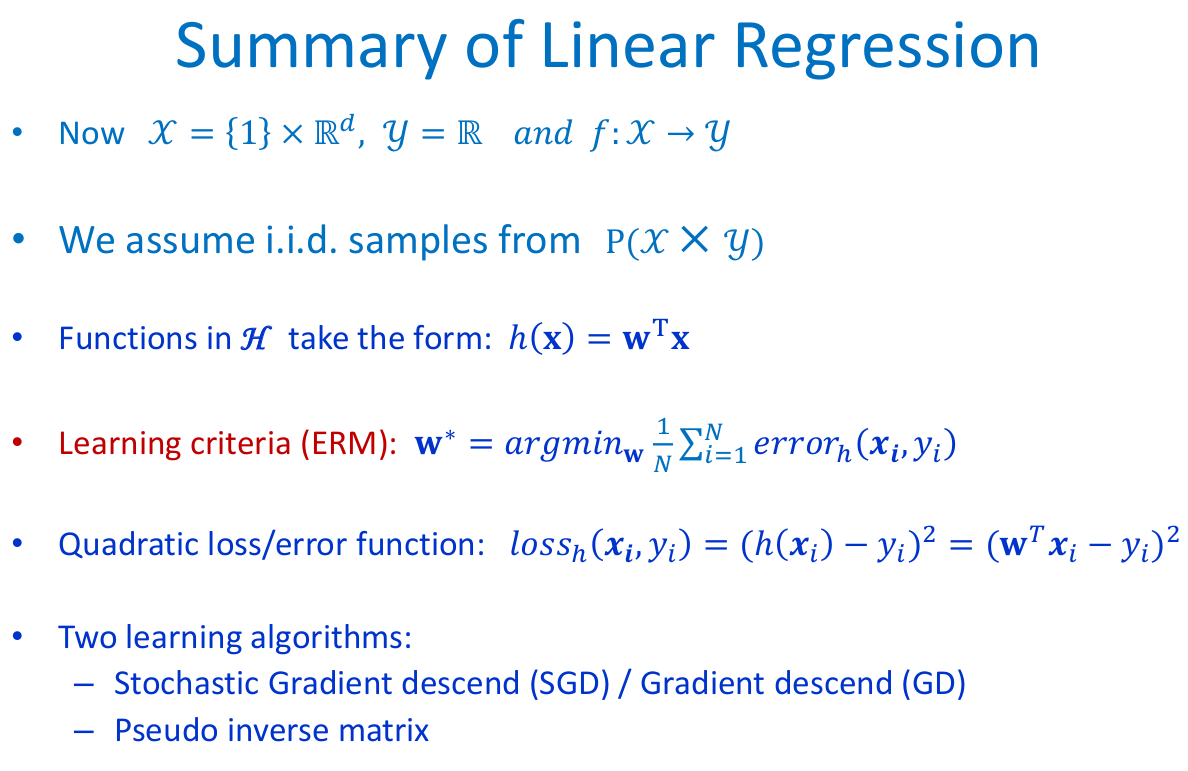
\includegraphics[width=0.75\textwidth]{images/summary_linear_regression}
	\caption{Summary Linear Regression}
	\end{figure}
	
	\subsubsection{En la práctica.}	
	Veamos algunos detalles prácticos. Éstos tienen que ver con la inferencia estadística, que trata de hacer inferencia sobre parámetros cuando las muestras son relativamente pequeñas (parte de estas técnicas de inferencia estadística no son aplicables en grandes cantidades de datos). En estas muestras relativamente pequeñas cualquier desviación de datos puede tener influencia en la estimación. Sin embargo en aprendizaje desde datos se está suponiendo que las muestras son de un tamaño especialmente grande. En cuyo caso muchos de estos fenómenos dejan de tener influencia.
	
	Recordemos las hipótesis básicas que tenemos en un modelo de regresión
	\begin{itemize}
		\item 
		\begin{itemize}
		\item Nosotros elegimos un vector de características $X=(X_1,...,X_n)\colon \Omega \to \R^d$. Al tomar una muestra podíamos tener errores, $Y_i=X_i^T \beta + \varepsilon_i$, $i=1,...,N$, y esos errores $\varepsilon_i$ se suponen incorrelados.
		\item También suponemos que las variables de $X=(X_1,...,X_n)$ son independientes, cada una aporta una información independiente de la otra. En la práctica puede que haya variables dependientes una de la otra, porque cuando las tomamos de la muestra estamos asumiendo que son independientes pero no lo sabemos (hay técnicas que descubren esas variables y técnicas que las eliminan para que el ajuste sea más correcto; suelen ser para tamaños de muestra pequeño o mediano, para tamaño grande son inviables -> nosotros lo haremos usando una técnica de ajuste global de la función pero no en detalle variable por variable)
		\item Algo que sí se puede aplicar a tamaños grandes son los conocidos como \textit{outliers}, es decir, observaciones que no siguen la distribución de la población. Son relevantes para muestras pequeñas pero para muestras muy grandes no son muy relevantes. A pesar de esto es importante en machine learning. Cuando terminamos de ajustar por regresión o modelo que sea, si es posible y siempre que sea posible se deben mirar aquellos datos en los que haya fallos de cierto calibre, para ver si esos datos tienen algún tipo de comportamiento que no se ha sabido modelar, o datos con valores que no corresponde y deban descartarse. Importante: esto último se hace una vez que hayamos terminado con el modelo, no antes.
	\end{itemize}
	
	\item ¿Qué variables es capaz el ordenador de manipular? Hay que saber codificar bien las variables para que el ordenador pueda operar correctamente.
	\begin{itemize}
		\item Las variables continuas se codifican con su propio valor.
		\item Si la variables es discreta, por ejemplo un color: verde, rojo..., ¿cómo codificar?. En variables continuas van a $\R$ y hay relación de orden. En variables categóricas no hay orden, no hay nada. Si se le asignase un número a cada color estaríamos estableciendo ya una relación de orden. Esto tiene una repercusión importante, se está ya estableciendo una relación de orden, algo que no existe.
		
		A las variables categóricas se les asignará un vector de tamaño $k$, el número de categorías, $(0,0,\ldots, 1,\ldots, 0)$ con un 1 en la posición de la categoría que toma nuestra variable. Esto será para cualquier situación en la que se usen variables categóricas. Se verá en Clasificación.
		
		Recordar que esto es en la práctica, fuera del modelo teórico. Se hace para poder operar de forma efectiva computacionalmente.
	\end{itemize}
	
	\item Otro problema. A veces hay valores perdidos en un $(x_1,...,x_d)$ vectores muestrales. Una solución es eliminarlo, eliminar el ítem. Pero puede ser que tengamos un porcentaje no despreciable de ítems así. ¿Qué se puede hacer? depende mucho de la técnica que estemos usando, hay técnicas en que los valores perdidos tienen muy poca importancia, porque son técnicas que construyen los procesos de decisión, ya sea regresión o clasificación, no haciendo combinaciones lineales de lso valores medidos...; si no usando los propios valores medidos uno a uno y tomando decisiones sobre ellos (por ejemplo los árboles, ya se verán). Entonces en estos casos la influencia es menor, pero cuando la clase de funciones está constituida por una combinación lineal de todas la variables $\Rightarrow$ si en una variable no hay valor esto tiene una influencia. Deberíamos sustituir ese valor por algo representativo, no son técnicas ni buenas ni malas, si nos falta la variable de la tercera posición, podríamos ver la distribución de esa variable. Asociar la moda, la media... (no es lo que toca, es preferible a poner algo que no toca o nada pero hay que saber que no es lo que realmente corresponde). Hay veces que se puede construir un pequeño problema de regresión para estimar ese valor a partir de los demás (no es lo habitual).
	
	\end{itemize}
	
	\subsection{Clasificación}
	Ahora no tenemos variable continua como en Regresión. Ahora el objetivo es asignar a cada ítem una clase (variable discreta).
	
	Por ejemplo, tenemos el conjunto de datos 
	
	\begin{figure}[H]
	\centering
	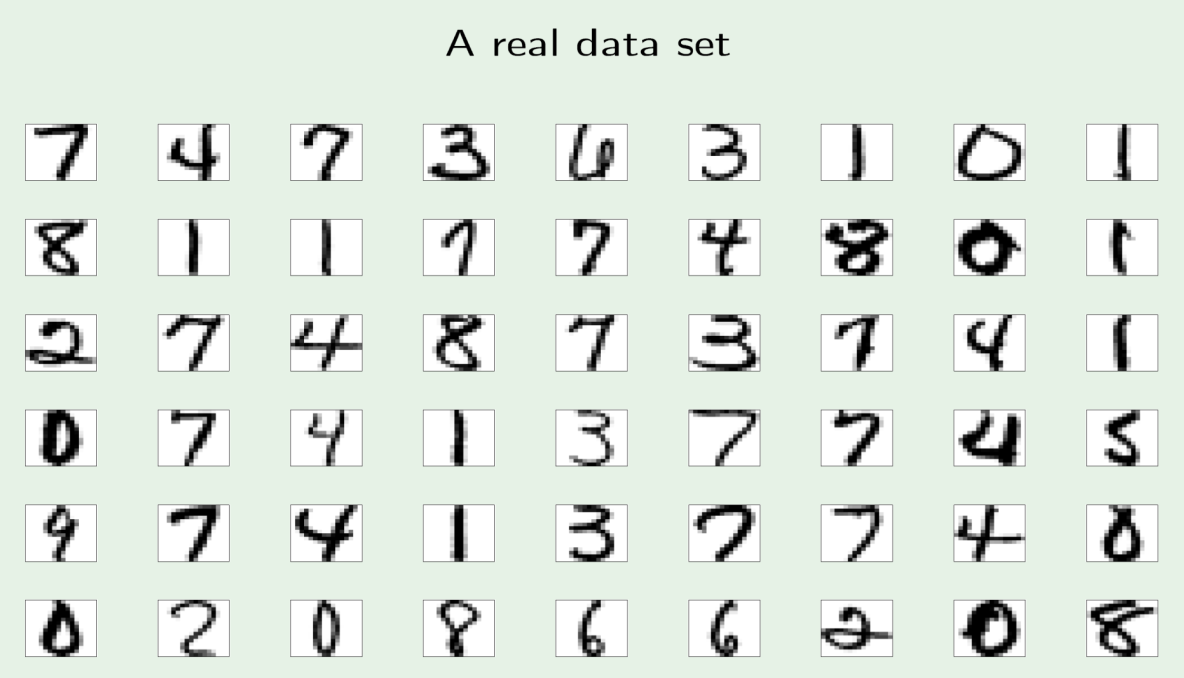
\includegraphics[width=0.55\textwidth]{images/ejemplo_classification}
	\caption{Ejemplo, imágenes de dígitos}
	\end{figure}
	
	y el problema de aprendizaje consiste en aprender a clasificar dígito por imagen. La entrada sería la imagen, la salida: que de 0 a 9 diese un número o diese un vector con todo 0 y un 1 en la casilla con posición correspondiente al número.
	
	¿Qué características vamos a extraer? (se podría no extraer ninguna característica y trabajar directamente con los píxeles como características; hay sistemas para hacer esto)\\
	Nosotros vamos a suponer que podemos utilizar características más significativas que nos permitan resolver el problema sin tener que usar los píxeles. Esto permite que el modelo sea más simple. 
	
	Por ejemplo, podemos tener imagen con 256 píxeles, entonces el modelo tendría entradas de 256+1 características $x=(x_0,x_1,\ldots, X_{256})$, y para el modelo tendríamos 256+1 parámetros $(w_0,w_1,\ldots,w_{256})$, se complica el modelo.\\
	Para evitar esta complicación simplificamos. Podemos extraer intensidad (nivel medio de gris) y simetría (sería vertical, si se divide con línea horizontal, mide la diferencia ``al doblar la imagen''), tendríamos $x=(x_0,x_1,x_2)$ y vectores de pesos $(w_0,w_1,w_2)$.
	\begin{figure}[H]
	\centering
	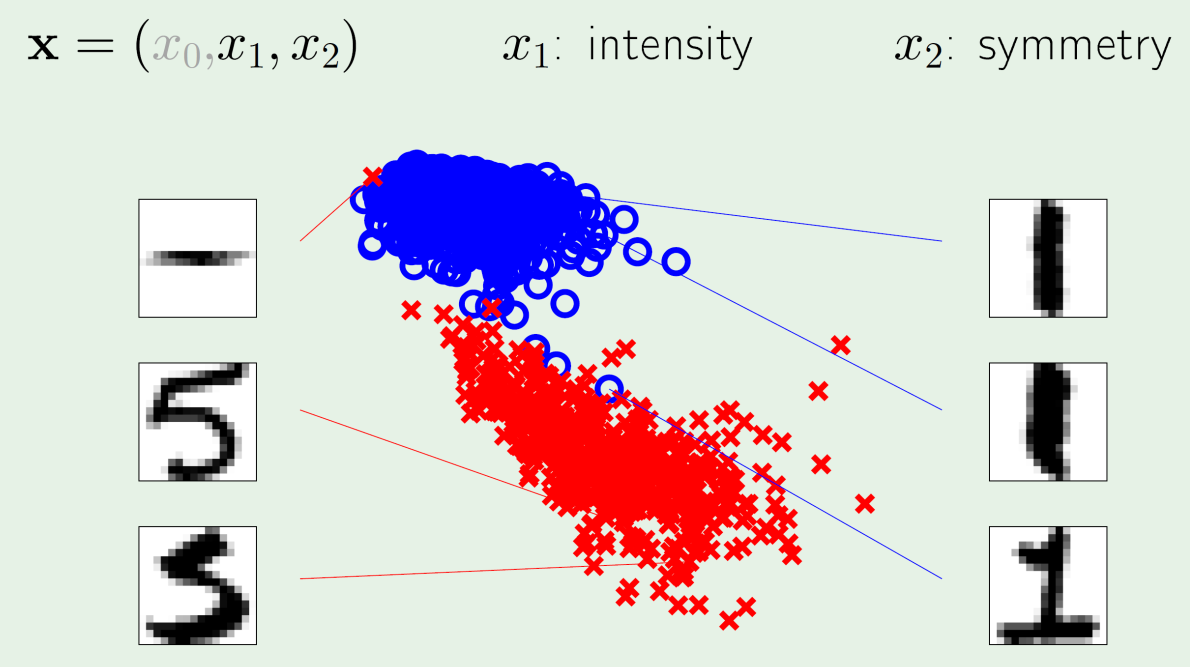
\includegraphics[width=0.55\textwidth]{images/inten_sim}
	\caption{Modelo con intensidad y simetría, para 1 y 5}
	\end{figure}
	Con intensidad y simetría no obtenemos un modelo perfecto pero no es malo.
	
	Nuestro será objetivo será encontrar un hiperplano ($\mathcal{H}$ clase de funciones de hiperplanos), que clasifique en dos categorías.
	\begin{figure}[H]
	\centering
	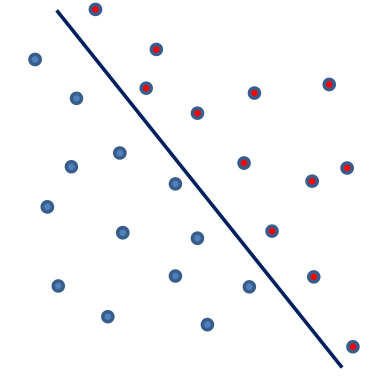
\includegraphics[width=0.3\textwidth]{images/clasifi}
	\caption{Hiperplano que clasifica en dos categorías}
	\end{figure}
	
	Entremos ahora en detalle, se definirá un modelo de aprendizaje (espacio de funciones hipótesis y algoritmo de aprendizaje), con el ejemplo de concesión de crédito:\\
	Sea $\mathcal{X}=\R^d$ el espacio de entrada, $\mathcal{+1,-1}$ el espacio de salida, denotando una decisión (sí/no). En nuestro ejemplo de crédito, las diferentes coordenadas de $x\in \R^d$ corresponden a salario, años de residencia, deuda pendiente,... . La salida binaria de $y$ corresponde a aprobar o no el crédito. Se especifica $\mathcal{H}$ mediante la propiedad que deben cumplir las funciones. La forma funcional de $h(x)$ que se elige da diferentes pesos a las diferentes coordenadas de $x$, reflejando su importancia relativa en la decisión de crédito. Las coordenadas con sus pesos son transformadas en un ``puntaje de crédito'' y el resultado es comparado con un valor umbral. Si se sobrepasa el puntaje de crédito entonces se aprueba, en otro caso se rechaza.
	
	$$\text{Aprobar crédito si } \ \ \sum_{i=1}^d w_i x_i \geq \text{ umbral}$$
	$$\text{Denegra crédito si } \ \ \sum_{i=1}^d w_i x_i < \text{ umbral}$$
	Puede resumirse en 
	$$h_w(x)=sign \left( \left( \sum_{i=1}^d w_i x_i\right) + b \right)$$
	donde $sign(s)=1$ $\forall s\in \R_0^+$, $sign(s)=-1$ $\forall s \in \R^-$. \\
	Equivalentemente, si llamamos $$x^T=(1,x_1,x_2,\ldots ,x_d),\quad w^T=(\overbrace{w_0}^b, w_1,\ldots , w_d)$$	
	entonces
	\begin{definition}[\bf Clase de funciones hipótesis para clasificación binaria]
	$$\mathcal{H}=\{h_w\colon \R^{d+1} \to \R \ : \ h_w(x) = sign(w^Tx), \ w \in \R^{d+1}\}$$
	\end{definition}
	Ahora nos falta el algoritmo. Hemos visto el método de Pseudoinversa (ligado a minimizar $E_{in}(w)=\frac{1}{N}\norm{Xw-y}^2$). Para nuestra nueva función de error vamos a contar cuantos ítems están bien clasificados y cuántos están mal clasificados
	\begin{definition}[\bf Error en la muestra (Clasificación)]
	Para una muestra $(x_1,y_1),\ldots ,(x_N, y_N)$ de tamaño $N$ (cada $x_i$ es un vector $d$-dimensional), se define el error dentro de la muestra
	$$E_{in}(h_w):= \frac{1}{N} \sum_{n=1}^N [[h_w(x)\neq y_n]] \quad \quad \text{ dividir por N nos da el ``porcentaje'' de fallos}$$
	donde 
	$$[[sign(w^T x_n) \neq y_n]] = \begin{cases}
	1 & sign(w^T x_n)\neq y_n\\
	0 & sign(w^T x_n) = y_n
	\end{cases}
	$$
	Equivalentemente
	$$E_{in}(w):= \frac{1}{N} \sum_{n=1}^N [[sign(w^Tx_n)\neq y_n]]$$
	
	\end{definition}
	De nuevo el criterio de aprendizaje es \textit{ERM} (\textit{Empirical Risk Minimization})
	Tal vez podríamos aplicar el método de \textit{Gradiente Descendente Estocástico}, pero $[[sign(w^T x_n) \neq y_n]]$ no es derivable. Veamos como solucionar esto
	
	\textit{Nota:} utilizaremos algoritmo Perceptron, algoritmo que nos dará una solución correcta, correcta respecto de la muestra(puede llegar a obtener error 0 en la muestra), que no óptima (no tiene por qué serlo, no sabemos como se comportará en la población).
	
	\begin{proposition}[\bf Nueva función de error derivable]
	La función de error es 
	$$error(w^Tx_n,y_n)=[[sign(w^T x_n)\neq y_n]] = \begin{cases}1 & sign(w^T x_n)\neq y_n\\
	0 & sign(w^T x_n) = y_n
	\end{cases}$$
	Una nueva función de error derivable puede ser deducible
	$$error(w^Tx_n,y_n)=\begin{cases} 
	-y_n w^T x_n & sign(w^Tx_n)\neq y_n\\
	0 & sign(w^T x_n)=y_n
	\end{cases}$$
	Notar que $-y_n w^T x_n >0$ cuando $sign(w^Tx_n)\neq y_n$. Equivalentemente
	$$error(w^T x_n, y_n)=\max \{0, -y_n w^T x_n\}$$
	
	\end{proposition}
	
	\begin{definition}[\bf Perceptron Learning Algorithm (PLA)]
		Llamamos \textit{Algoritmo de Aprendizaje Perceptron} al caso particular del algoritmo \textit{Gradiente Descendente Estocástico} para tamaño batch 1 y tasa de aprendizaje 1 para la función $error(w^T x_n, y_n)=\max \{0, -y_n w^T x_n\}$
		
		La regla de adapación del algoritmo es 
		$$\begin{cases}
		w_{updated} = w_{current} +y_ix_i & sign(w^Tx_i) \neq y_i\\
		w_{updated} = w_{current} & sign(w^Tx_i) = y_i
		\end{cases}$$
		el pseudocódigo queda
		
	\begin{figure}[H]
	\centering
	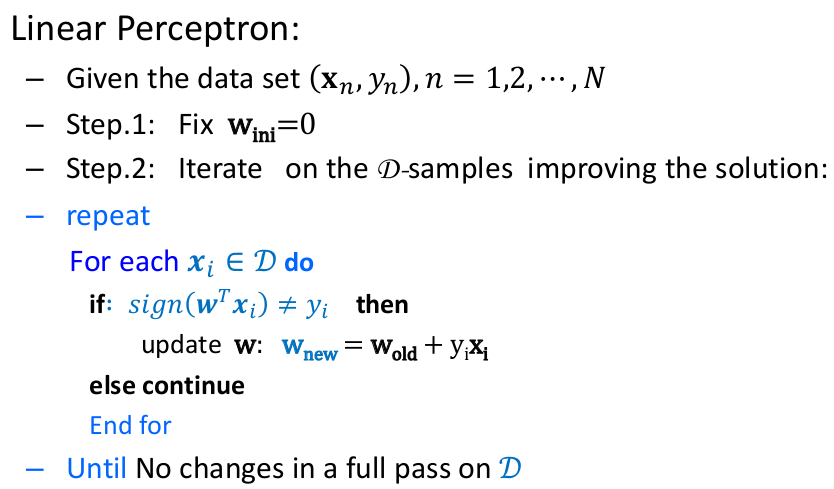
\includegraphics[width=0.55\textwidth]{images/perceptron_alg}
	\caption{Pseudocódigo del algoritmo Perceptron}
	\end{figure}
	
	Notar que este algoritmo de aprendizaje itera en los datos muestrales ``sin memoria''. En el paso 1 realmente se quiere decir $w_{ini} \approx 0$, vector de pesos con valores pequeños pero no el vector 0, si fuese 0 no se movería.
	\end{definition}
	
	\begin{proposition}[\bf Propiedades del algoritmo Perceptron]
	El algoritmo busca la mejor $h\in \mathcal{H}$ a través de evaluaciones iterativas en los datos de entrenamiento $\mathcal{D}$. Si tenemos un conjunto de datos de entrenamiento $\mathcal{D}$ separable (existe hiperplano que separa los puntos de cada clase), entonces el algoritmo PLA encuentra vector de pesos, $\hat w$, con $h_{\hat w}(x_i)=y_i$ para todos los $(x_i,y_i)$ de $\mathcal{D}$ en tiempo finito.
	
	\end{proposition}
	
	\textit{Nota:} de momento la intuición de las combinaciones lineales nos encajan, pero aumentaremos las variables y el concepto de linealmente separable puede ya no encajar con la intuición. Linealmente separable pueden ser polinomios de 3er 4to orden.
	
	\underline{Error PLA}\\
	El error puede ir variando, cuando se modifica el hiperplano porque un dato no estaba bien clasificado puede que hagamos que dos o más datos que sí estaban bien clasificados pasen a estar mal clasificados. Por tanto los errores van variando mucho, no hay una sucesión decreciente en los errores, lo que sí podemos saber es que si $\mathcal{D}$ es separable $\Rightarrow$ acabaremos con error 0 dentro de la muestra.
	
	\begin{figure}[H]
	\centering
	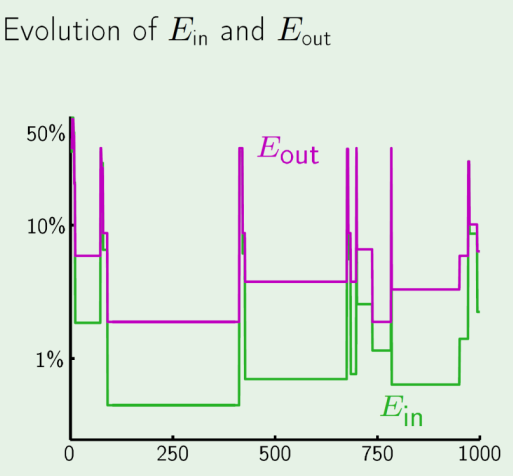
\includegraphics[width=0.35\textwidth]{images/error_pla}
	\caption{Error del algoritmo Perceptron}
	\end{figure}

	Muchas veces tenemos que poner un máximo de iteraciones, no sabemos si es separable. Depende del número de iteraciones máximo podemos obtener una mejor o peor solución. Puede que la iteración 500 tengamos una muy buena solución y en la 700 mala. El error no decrece con el número de iteraciones.	
	\begin{figure}[H]
	\centering
	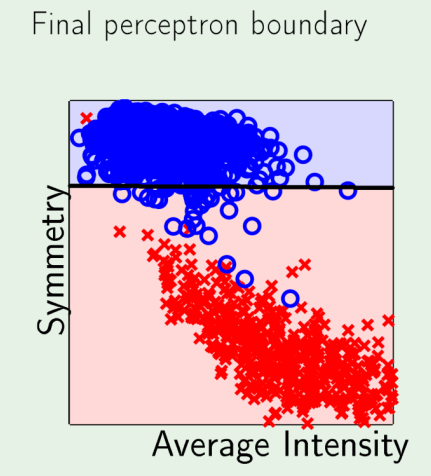
\includegraphics[width=0.35\textwidth]{images/percep_boundary}
	\caption{Parada por iteraciones en algoritmo Perceptron}
	\end{figure}
	\begin{proposition}
	Supongamos que llegamos a una aproximación $g$ de $f$ mediante el algoritmo PLA, entonces
	$$E_{out}(g)\leq E_{in}(g) + \mathcal{O}\left(\sqrt{d\frac{\log N}{N}}\right)$$
	por lo que, para $N$ suficientemente grande, $E_{out}$ estará acotado por $E_{in}$ 
	\end{proposition}~\\
	
	\underline{¿Podemos conseguir $g$ tal que $E_{in}(g) \approx 0$?} Dos escenarios:
	
	\begin{enumerate}
	\item \textbf{Escenario 1} - Datos linealmente separables.\\
	Es decir existe $w^*$ con $E_{in}(w^*)=0$
	\begin{proposition}[\hypertarget{plaResult}{\bf PLA-Result}]
		Sea $(x_1,y_1),\ldots,(x_N,y_N)$ una muestra separable. Sea $B=\min_{w\in R^{d+1}} \{\norm{w} \ : \ y_i w^T x_i \geq 1 \quad \forall i \in \{1,\ldots,N\}\}$, y sea $R=\max_{i\in \{1,\ldots,N\}} \norm{x_i}$. Entonces PLA para en un máximo de $(RB)^2$ iteraciones, y cuando para se verifica  $y_iw^Tx_i \geq 0$ $\forall i \in \{1,\ldots, N\}$
	\end{proposition}
	\item \textbf{Escenario 2}- Datos no separables.\\
	Dos posibilidades o escenarios
	\begin{itemize}
	\item \textbf{NS.1:} existe solución lineal separable con errores.\\ 
	Recordar que este estas dos soluciones son lineales, en la segunda imagen se utilizan también los cuadrados de las características (es lineal porque es $w$ multiplicado por algo)
	\begin{figure}[H]
		\centering
		\begin{subfigure}{.3\textwidth}
  		\centering
  		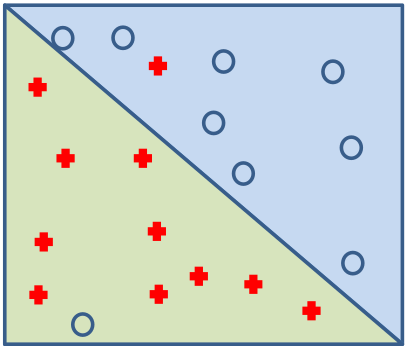
\includegraphics[width=1\textwidth]{images/non_sep_rectaa}
  		\caption{Separable con ciertos, pocos, errores.}
  		\label{fig:sub1}
		\end{subfigure}%
		\begin{subfigure}{.287\textwidth}
  		\centering
  		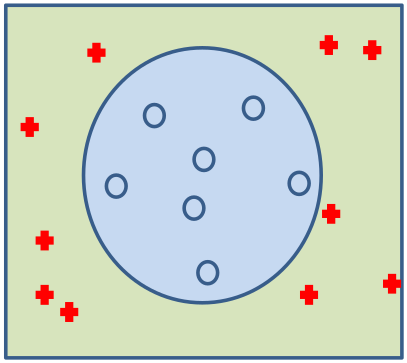
\includegraphics[width=1\textwidth]{images/non_sep_elipse}
  		\caption{No se consigue error bajo por hiperplanos}
  		\label{fig:sub2}
		\end{subfigure}
		\caption{}
		\label{fig:test}
	\end{figure}
	En el primer caso se distingue del segundo porque podemos, con ciertos errores, tener una solución por hiperplano. Tenemos un hiperplano que representa razonablemente bien la separación aunque hay algunos errores. Cuando se pueda dar una solución por combinación lineal de las observaciones, aún con algunos errores, es mejor dar esta solución.
	
	Aunque en este caso, sabemos que si utilizamos Perceptron no va a terminar. Para solucionar esto se usa Pocket Algorithm.\\
	
	\textbf{Algoritmo Pocket:} mantiene, va guardando, el mejor vector solución encontrado en la iteración $t$ de PLA.
	\begin{figure}[H]
	\centering
	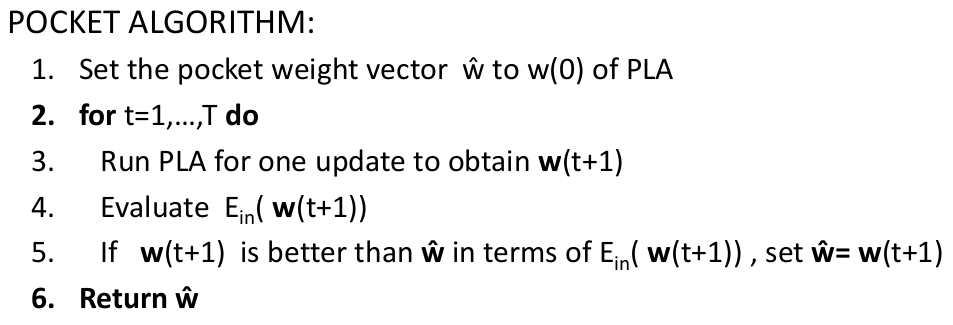
\includegraphics[width=0.6\textwidth]{images/pocket}
	\caption{Pseudocódigo Pocket Algorithm}
	\end{figure}
	\textit{Nota:} tiene baja eficiencia en paso 4. Lo bueno es que garantiza una buena solución después de un número alto de iteraciones.\\
	Al ir solo actualizando si hay una solución mejor, el error va disminuyendo con las iteraciones
	\begin{figure}[H]
	\centering
	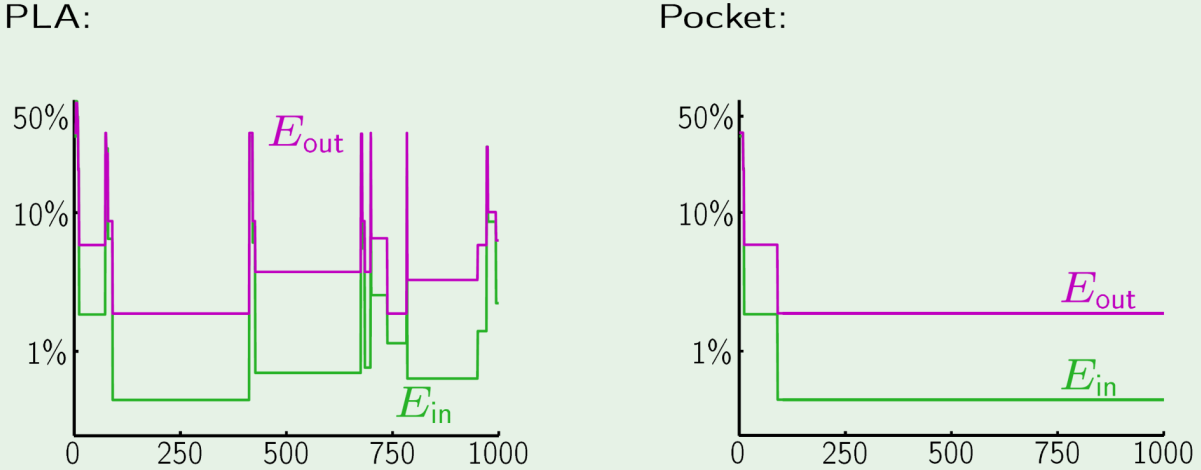
\includegraphics[width=0.6\textwidth]{images/error_pocket}
	\caption{Errores Pocket Algorithm y PLA}
	\end{figure}
	Posibles resultados cuando no existe solución por hiperplano sin errores (PLA tendríamos que pararlo tras un número de iteraciones porque no acaba.
	\begin{figure}[H]
	\centering
	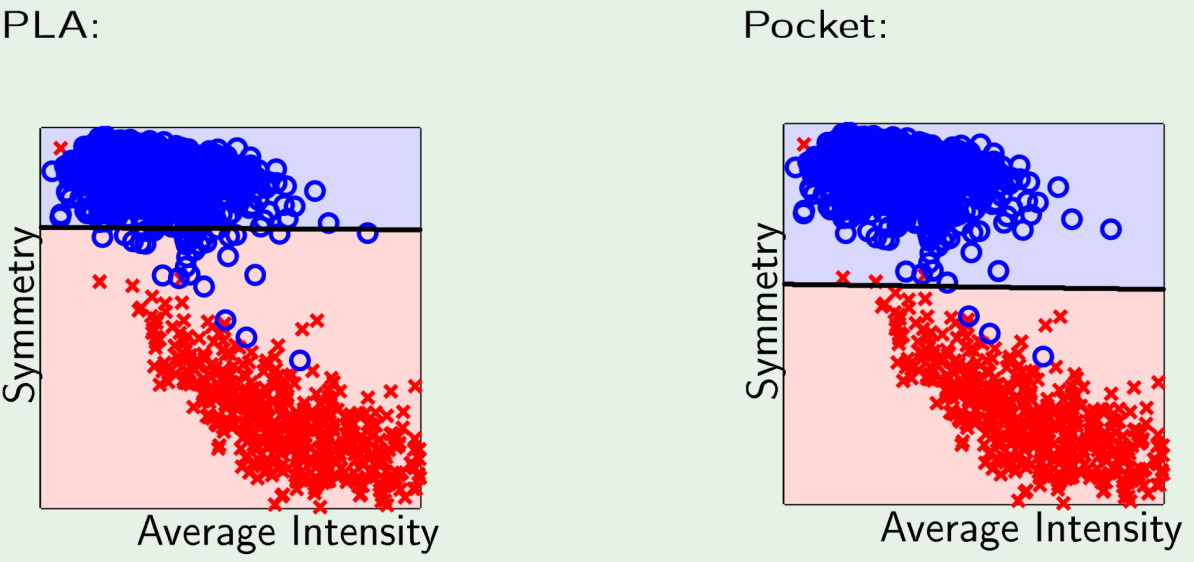
\includegraphics[width=0.6\textwidth]{images/pla_vs_pocket_sol}
	\caption{Classification boundary - PLA vs Pocket}
	\end{figure}
	\item \textbf{NS.2:} No existe una solución lineal separable\\
	En el segundo caso no hay error bajo para ningún hiperplano, siempre habrá error alto. En este caso se amplía a una clase de funciones que sigue siendo lineal pero más rica. Se añaden transformaciones no lineales de los datos. (se verá más adelante)
	\end{itemize}
	\end{enumerate}

	Por cómo es la función de pérdida no podemos usar método de Regresión Lineal como Pseudoinversa (no resolvemos analíticamente, hay que iterar), sí podemos usar Gradiente descendiente (PLA es caso particular). 
	
	¿Puede la Regresión ayudar a clasificar?
	Sí, el valor de regresión es un buen comienzo, nos puede dar una solución inicial para luego iterar a partir de ella. Hay que interpretar nuestro problema de clasificación como uno de regresión. En el caso binario es muy simple.
	\begin{itemize}
		\item Regresión lineal aprende una función $f(x)=y\in \R$. Las funciones con evaluación binaria también tienen rango real, $\pm 1\in \R$
		\item Utilizar regresión lineal para obtener $w$ con $w^T x_n \approx y_n = \pm 1$
		\item En este caso $sign(w^T x_n)$ es probable que sea una aproximación de $y_n=\pm 1$
		\item Así obtenemos, en general, un buen vector de pesos inicial para clasificación.
	\end{itemize}
	
	\subsection{Noisy labels}
	Hasta ahora asumíamos una función $f$ determinista, a cada elemento de la muestra le asigna una etiqueta. Ahora vamos a suponer que no, vamos a suponer que la función $f$ es una probabilidad. Esto es más normal, lo difícil es que $f$ sea determinista.
	
	En ejemplos reales lo natural es $f$ una probabilidad y no una función determinística.
	
	Normalmente usamos un vector de características. ¿Quién nos dice que ese vector representa toda la información necesaria para determinar las etiquetas? No lo podemos saber, lo normal es que haya ruido, factores/variables que no se tienen en cuenta. Y lo natural sea pensar en una probabilidad.
	
	Ejemplos:
	\begin{itemize}
		\item Credit approval case: two customers with identical data can have different answer.
		\item Tasty mangos: items with the same features can be labeled as of different class.
	\end{itemize}
	
	\underline{Ejemplo:} Suppose we want to predict the ocurrence of heart attacks based on a person's cholesterol level, blood pressure, age, weight, and other factors. Obviously, we cannot predict a heart attack with any certainty, but we may be able to predcit how likely it is to occur givn these factors. Therefore, an output that varies continuously between 0 and 1 would be a more suitable model than a binary decision. The closer $y$ is to 1, the more likely that the person will have a heart attack.\\
	
	Si con +1 denotamos el tener ataque al corazón, lo natural pensar en buscar aproximar $f(x)=P(y=+1|x)$. Aquí hay etiquetas ruidosas, bajo misma $x$ tenemos una probabilidad $f(x)=P(y=+1|x)$, habrá veces que bajo misma $x$ ocurra o no ocurra $y=+1$. Esto es por que hay factores, variables aleatorias no incluidas en vector características (esto es pensando en términos deterministas), o una aleatoriedad no controlable.\\
	
	Ahora hay que introducir la probabilidad.\\
	Cambios:
	\begin{itemize}
	\item En vez de pensar que dado un $x$ podemos saber $y$ mediante una función, $f$, determinista $y=f(x)$ (determinista), ahora buscamos una función $f$ que estime la probabilidad de que ocurra $y$ dado un $x$, $f(x)=P(y=1|x)$\\ Nota: $f\colon \mathcal X \to \mathcal Y$, $y\colon \Omega \to \mathcal Y=y(\Omega)$, $x\colon \Omega \to \mathcal X = x(\Omega)$ y $f(x)\colon \Omega \to \mathcal Y$
	\item Cada elemento de la muestra $(x,y)$ es generado de la distribución conjunta $P(x)P(y|x)$ que no es más que $P(x,y)$
	\item Noisy target (etiquetas ruidosas), que no es más que unas etiquetas deterministas por $\psi(x)=E(y|x)$, más un ruido $y-\psi(x)$
	\item $P(x,y)=P(x)P(y|x)$, queremos aprender $P(y|x)$, $P(x)$ cuantifica la importancia relativa de $x$
	\item $P(x,y)=P(x)P(y|x)=P(x|y)P(y)$. Claramente si conocemos $P(x,y)$ no hay nada que aprender. Nosotros buscaremos $P(y|x)$, hay otros enfoques que buscan $P(x|y)$, conocer la probabilidad de la muestra sabiendo $y$. Conocer $P(x|y)$ da otro método para computar $P(y|x)$, ahora se ve
	\item Formas de conocer $P(y|x)$
	\begin{itemize}
		\item Aprender $P(y|x)$ directamente (Abordaje discriminativo). Discriminan las clases, separan las clases.
		\item Conocer $P(y|x)$ conociendo $P(x|y)$ usando la regla de Bayes (Abordaje generativo). Tratan de entender el fenómeno que está generando las muestras.
		$$P(y|x)=\frac{P(x|y)P(y)}{P(x)}$$
		
		Conocer $P(x|y)$ es más complejo que conocer $P(y|x)$ directamente. Aunque conocer $P(x|y)$ puede dar más valor intuitivo de qué está pasando. Se necesitan bastantes más datos para conocer $P(x|y)$ que para conocer $P(y|x)$ por el método directo
	\end{itemize}
	Hoy en día tiene más popularidad el Abordaje discriminativo. Métodos como redes neuronales son técnicas para conocer $P(y|x)$ directamente. En adelante, en \textit{Regresión Logística}, usaremos abordaje discriminativo, buscaremos conocer $P(y|x)$ directamente.
	\end{itemize}
	
	\begin{figure}[H]
	\centering
	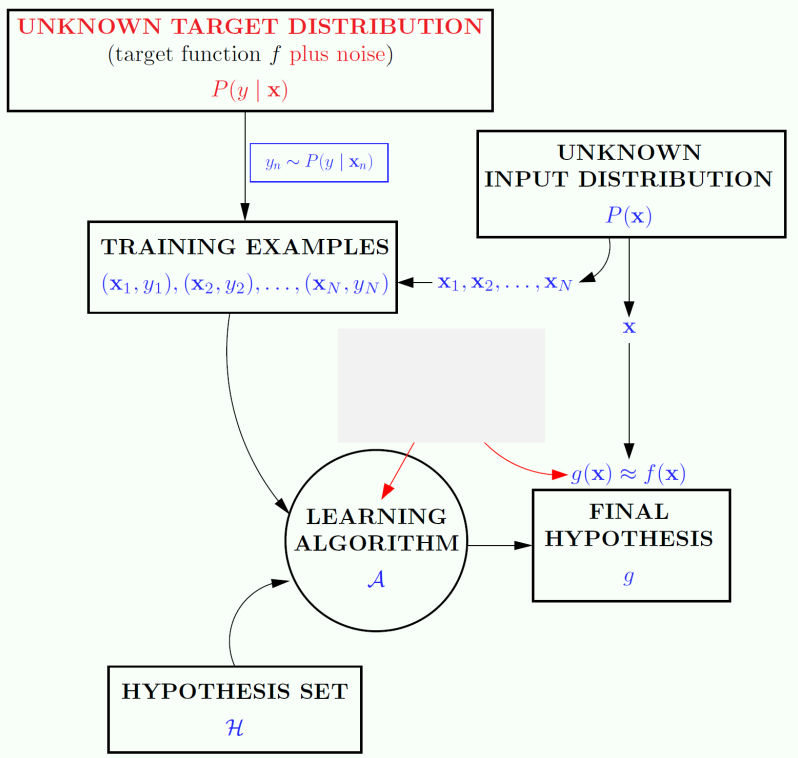
\includegraphics[width=0.6\textwidth]{images/updated_learning_P}
	\caption{Updated Learning Schema - Probability}
	\end{figure}
	
	\subsection{Regresión Logística (LGR) - Estimación por Probabilidad.}
	Regresión porque clasificamos pero con probabilidad y por tanto el rango es continuo.
	
	Para \textit{Regresión Logística} binaria utilizaremos las etiquetas $\{-1,1\}$ por conveniencia a la hora de formular las ecuaciones.
	\subsubsection{Regresión Logística binaria, $y=\pm 1$, dos clases C1 y C2}
	Ahora la función $f\colon \mathcal{X} \to [0,1]$ es $f(x)=P(y=1|x)$
	\begin{definition}[\bf Clase de funciones hipótesis para Regresión Logística]
	$$\mathcal{H}:=\{h_w\colon \R^{d+1}\to \R \ :\ h_w(x)=\sigma(w^Tx),\ w \in \R^{d+1}\}$$
	donde $\sigma$ es la función logística (sigmoide), $\sigma\colon \R \to [0,1]$, $\sigma(x)=\frac{1}{1+e^{-x}}=\frac{e^x}{e^x+1}$
	\begin{figure}[H]
	\centering
	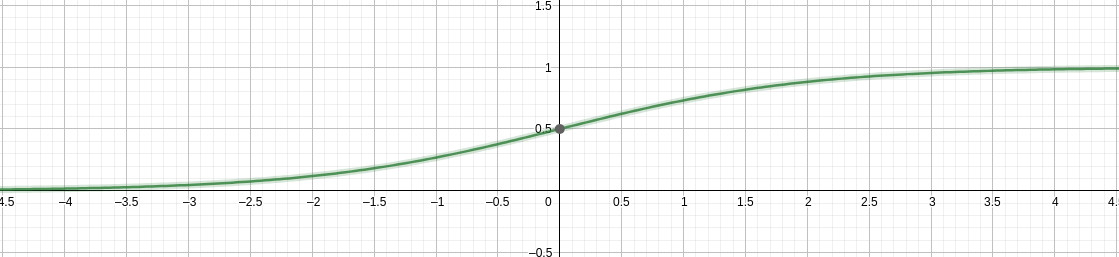
\includegraphics[width=0.6\textwidth]{images/sigmoide}
	\caption{Sigmoide function}
	\end{figure}
	también pude considerarse otra función $\tanh \colon \R \to [-1,1]$, $\tanh(x)=\frac{e^x-e^{-x}}{e^x+e^{-x}}$
	\begin{figure}[H]
	\centering
	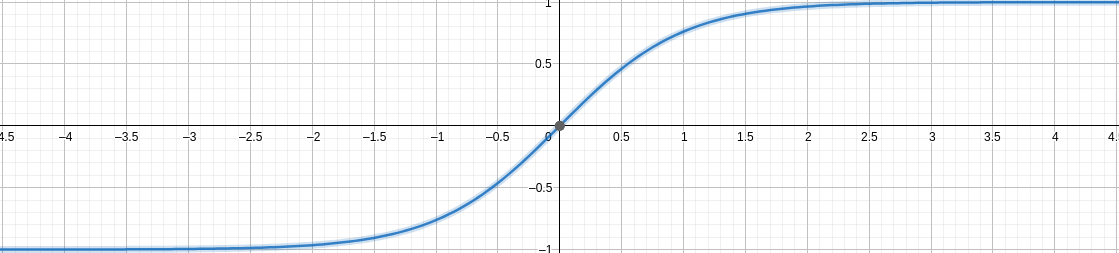
\includegraphics[width=0.55\textwidth]{images/tanh}
	\caption{tanh}
	\end{figure}
	\end{definition}
	
	\begin{proposition}[\bf Prop. antes de ver error en la muestra]. 
	Por como hemos definido $f(x)$
	$$ P(y| x) = \begin{cases} f(x) & y=+1 \\
	1-f(x) & y=-1
	\end{cases}$$
	
	\begin{itemize}
	\item	Mediante $\sigma$ podemos considerar que estamos trabajando con probabilidad. Dado $h_w \in \mathcal{H}$
	$$h_w(x)=\sigma(w^Tx)=\frac{e^{w^Tx}}{1+e^{w^Tx}}\quad \ \ \text{C1 probability}$$
	$$1-h_w(x)= 1-\sigma(w^T x) =\sigma(-w^Tx)=\frac{1}{1+e^{w^Tx}} \quad \ \ \text{C2 probability}$$
	si $h_w \approx f$
	$$P(y| x)\approx \begin{cases} h_w(x) & y=+1\\
	1 - h_w(x) & y=-1
	\end{cases} \quad \quad (*)$$
	Podemos sustituir $h_w(x)$ por su valor $\sigma(w^Tx)$ y utilizar que $1-\sigma(w^Tx)=\sigma(-w^Tx)$ para obtener $$P(y|x)\approx \sigma(yw^Tx)$$
	\item A $\frac{h_w(x)}{1-h_w(x)}$ se le llama ``odds'' (es la proporción o número de veces que es más probable una clase que la otra). Si tomamos 
	$$\ln\left(\frac{h_w(x)}{1-h_w(x)}\right)=\ln\left(e^{w^T x}\right)=w^Tx$$
	obtenemos una función, función \textit{logit}, del tipo de funciones hipótesis de modelo de regresión lineal.
	\end{itemize}
	\end{proposition}
	
	Idea subyacente: ``Supongamos que tenemos $h_w \in \mathcal H$. Supogamos que $h_w=f$, ¿cuál sería la probabilidad de obtener los datos de la muestra con la que he trabajado, $(x_1,y_1),\ldots,(x_N, y_N)$, si mi hipótesis es cierta? Si es baja entonces nuestra $h_w$ no es muy buena y sí puede ser plausible, la función hipótesis $h_w$, si la probabilidad es alta'' Así tenemos un criterio para decidir si una función hipótesis es más plausible que otra.
	
	\begin{definition}[\bf Error dentro de la muestra]
		 En general, dada una muestra $(x_1,y_1),\ldots,(x_N, y_N)$ i.i.d, la probabilidad de obtener todos los $y_i$ correspondientes a los $x_i$ es
		$$\prod_{n=1}^N P(y_n | x_n)$$ 
		Suponemos que tenemos una muestra $(x_1,y_1),\ldots,(x_N, y_N)$ y una función hipótesis $h_w(x)=\sigma(w^Tx)$, queremos ver cómo de buena es $h_w$ para la muestra.
		
		El método \textit{maximum likelihood} selecciona la función hipótesis $h_w$ que maximiza esta probabilidad vista como función de $w$, es decir queremos maximizar (recordar (*) para lo siguiente)
	$$L(w)\iffalse=\prod_{i=1}^N P(y_i|x_i)\fi=\prod_{i=1}^N \sigma (y_i w^T x_i) = \prod_{j=1}^{N_1}\sigma (w^T x_j) \prod_{k=1}^{N_{-1}} \sigma(-w^Tx_k)$$
		Como $-\frac{1}{N} \ln()$ es decreciente, maximizar $L(w)$ equivale a minimizar (aquí $P$ realmente es $\sigma$ la estimación de la verdadera $P$, abuso de notación)
		$$-\frac{1}{N} \ln\left( \prod_{n=1}^N P(y_n| x_n)\right)=\frac{1}{N} \ln\left( \prod_{n=1}^N \frac{1}{P(y_n| x_n)}\right)=\frac{1}{N} \ln\left( \prod_{n=1}^N \frac{1}{\sigma(y_n w^T x_n)}\right)=\frac{1}{N} \ln\left( \sum_{n=1}^N \frac{1}{\sigma(y_n w^T x_n)}\right)$$
		Sustituyendo la función sigmoide por su expresión, tenemos finalmente
		$$E_{in}(w):=\frac{1}{N} \sum_{n=1}^N \ln \left(1+e^{-y_nw^Tx_n}\right)$$
		Si $e(h_w(x_n),y_n)=\ln (1+e^{-y_nw^T x_n})$, podemos ver que $e(h_w(x_n),y_n)$ es valor pequeño, y positivo siempre, cuando $y_iw^Tx_i$ es grande.
	\end{definition} 
	
	\underline{Minimizando $E_{in}$}\\
	
	Vemos que 
	$$\nabla E_{in}(w)=\frac{\partial}{\partial w} \left( \frac{1}{N} \sum_{i=0}^N \ln (1+e^{-y_i w^T x_i})\right)=\frac{1}{N}\sum_{i=0}^N -y_ix_i \frac{e^{-y_i w^T x_i}}{1+e^{-y_iw^Tx_i}}=\frac{1}{N}\sum_{i=0}^N -y_ix_i\sigma(-y_iw^Tx_i)$$
	
	Para calcularlo podemos usar \textit{SGD}
	
	\begin{proposition}
		Si las etiquetas son 0 y 1 en vez de -1 y 1, podemos reescribir $L$ como
		$$L(w)= \prod_{i=1}^N \sigma (w^Tx_i)^{[[y_i==1]]}(1-\sigma(w^Tx_i))^{[[y_i==0]]}=\prod_{i=1}^N \prod_{k=0}^1 \sigma(w^Tx_i)^{y_{ik}}$$
	\end{proposition}
	\subsubsection{Regresión Logística multiclase o multietiqueta}
	\begin{proposition}
		Sea $x$ es una variable aleatoria de Bernoulli con $P(x=1)=p$ y $P(x=0)=q$, $p+q=1$, y $(x_1,\ldots,x_N)$ muestra iid
		\begin{itemize}
		\item $P(x)=p^xq^y$, $y=1-x$, $x\in \{0,1\}$
		\item $P(x_1,x_2,\ldots, x_N)=\prod_{i=1}^N P(x_i)=p^{\sum x_i} q^{\sum y_i}=p^{\#[x=1]} q^{\#[x=0]}$\\
		$x_1,\ldots,x_N$ v.a.
		\item Si $w$ está dado, para nuestra aproximación de probabilidad tenemos la expresión $$L(x_1,x_2,\ldots, x_N)=\prod_{i=1}^N \sigma(w^T x_i)^{[[x_i==1]]} (1-\sigma(w^Tx_i))^{[[x_i==0]]}=\prod_{i=1}^N \prod_{k=0}^1 \sigma (w^T x_i)^{y_{ik}}$$\\ que nos puede ser útil pues nos da una fórmula general que servirá para varias clases.\\ Aquí $(x_1,x_2,\ldots, x_N)$ son valores de muestra, querremos convertir en algo como v.a., algo que calcule probabilidades
		\end{itemize}
	\end{proposition}
	
	La regresión logística binaria puede ser generalizada a $K$ etiquetas o clases. A partir de ahora suponemos que tenemos $K$ etiquetas o clases.
	
	Ahora las etiquetas, denotadas por $y$ son representadas por un vector de $K$ componentes, $[0,0,\ldots,1,\ldots ,0]$ o también se podría usar $[-1,-1,\ldots,1,\ldots,-1]$
	
	\begin{proposition}[\bf Independencia condicional para muestra]
		Supongamos $w_1,\ldots, w_K$ con $w_i$ vector que define hiperplano que separa la clase $i$ del resto. $w_i\colon \Omega \to \R^{d+1}$, cada $w_i$ se considera como vector aleatorio \\
		Sea $(x,y)$ un elemento de muestra ($x\colon \Omega \to \R^{d+1}$, $y\colon \Omega \to \R^K$), y supongamos independencia condicional
		$$P(y| w_1,\ldots , w_K,x)=\prod_{k=1}^K P(y_k | w_k, x)= \prod_{k=1}^K \sigma(w_k^T x)^{y_k}$$
		Si tenemos $(X,Y)$ una muestra iid de tamaño $N$, $X=(x_1,\ldots,x_N)$, $Y=(y_1,\ldots,y_N)$, la independencia condicional queda
		$$P(Y|w_1,\ldots,w_K, x_1,\ldots,x_N)=\prod_{n=1}^N\prod_{k=1}^K P(y_{nk} |w_k,x_n)$$
	\end{proposition}
	
	\begin{definition}
		La verosimilitud (likelihood) se define como
		$$L(Y| w_1,\ldots, w_K)=\prod_{n=1}^N\prod_{k=1}^K \left(\sigma(w_k^Tx_n)\right)^{y_{nk}}$$
	\end{definition}
	
	\textit{Notación:}
	\begin{itemize}
		\item Dada una observación $x_n$, $n\in N$,
		$$t_{nk}:=\sigma(w_k^T x_n),\ \ \sum_{k=1}^K t_{nk}=1$$
		$\sum_{k=1}^K t_{nk}=1$ es una restricción que pondríamos en problema de optimización a la hora de calcular.
	\end{itemize}
	
	\begin{definition}[\bf Error dentro de la muestra]
		Queremos maximizar $L(Y|w_1,w_2,\ldots ,w_K)$ vista como función de $w_1,\ldots,w_K$, que equivale  a minimizar $-\ln L(Y|w_1,\ldots,w_K)$ como función de $w_1,\ldots ,w_K$
		$$E_{in}(w_1,\ldots,w_K):=-\ln L(Y|w_1,\ldots ,w_K)=-\sum_{n=1}^N \sum_{k=1}^K y_{nk} \ln t_{nk}$$
		la última expresión recibe el nombre, o se le llama: entropía cruzada entre las probabilidad reales de las observaciones de la muestra y las probabilidades que le asignan los valores de $w$ que nosotros teóricamente podemos ir estimando.
	\end{definition}
	
	\underline{Minimizando $E_{in}$}
	$$\nabla_{w_j} E_{in}(w_1,\ldots,w_K)=\sum_{n=1}^N (t_{nj}-y_{nj}) x_n$$
	
	\textit{Nota:} el gradiente ``camina'' mucho más rápido cuando la diferencia entre la etiqueta $y_{nj}$ y la predicción $t_{nj}$ es muy grande. Conforme se avanza el gradiente va disminuyendo.
	
	Supongamos que ya hemos acabado la optimización, terminaremos conociendo $w_1,\ldots ,w_k$. ¿Ahora qué?. Necesitamos asignar la observación a una clase concreta. Seguiremos el criterio SOFTMAX.
	
	\textbf{SOFTMAX:}\\ para cada vector de características $x$ un vector de probabilidades se computa usando los vectores estimados $w_1,w_2,\ldots,w_k$. Las componentes del vector son
	$$P(C_j|x)=\frac{exp(w_jx)}{\sum_k exp(w_kx)}, \quad j=1,\ldots ,K$$
	según \href{http://ufldl.stanford.edu/tutorial/supervised/SoftmaxRegression/}{web standford}
	$$P(y_i=j|x_i)=\frac{exp(w_j^Tx_i)}{\sum_{k=1}^K exp(w_kx_i)} \quad j=1,\ldots ,K$$
	
	\textbf{Decision Rule:}\\ Asignar $x$ a $C_j$ que verifique $P(C_j |x)=\max_{k\in \{1,\ldots, K\}} P(C_k|x)$. (asignar a la clase con mayor probabilidad, si el máximo no es único se asigna a cualquiera, no importa)\\
	
	Si conociéramos la verdadera distribución de probabilidad, $P$, ¿Podríamos generar una hipótesis óptima (hipótesis con mínimo riesgo) para cualquier tarea de aprendizaje? \\
	La Regla de Bayes nos justifica la Decision Rule de asignar a la clase más probable\\
	\textbf{Regla de Bayes:}
	Dada una distribución de probabilidad, $P$, conocida, la mejor función predictora de etiqueta de $x$ a $\{0,1\}$ es
	$$f_P(x)=\begin{cases} 1 & P[y=1|x]\geq \frac{1}{2} \\
	0 & \text{en otro caso} \end{cases}\quad \quad \text{(Regla de Bayes)}$$
	Además, no es difícil de probar, para cualquier distribución de probabilidad no existe otra función con menor riesgo que $f_P$, esto es, para cualquier otra función $g$, $E_{out}(f_P)\leq E_{out}(g)$
	
	\textit{Nota:} hay abordajes que primero estiman $P$ de las muestras y luego clasifican mediante la Regla de Bayes (Modelos Generativos, que son más terreno de la estadística). Pero estimar $P$ es mucho más complicado que el problema que nosotros queremos resolver que es saber si un ítem pertenece a una clase u otra. ``To solve a problem never solve a more complex one as intermediate step''
	
	
	\subsection{ERM}
	El objetivo siempre es minimizar el error dentro de la muestra para poder elegir una función hipótesis final con el menor error posible fuera de la muestra.
	
	Estamos utlizando el principio ERM (\textit{Empirical Risk Minimization}).
	
	\begin{definition}[\textbf{ERM} \href{https://en.wikipedia.org/wiki/Empirical_risk_minimization}{wiki} ] 
	Asumimos que tenemos una función de pérdida real-valuada no negativa $L(\hat y, y)$ que mide cómo de diferentes son la predicción $\hat y$ de una hipótesis (en nuestro caso $\hat y=h_w(x)$, con $x=(x_1,\ldots , x_d)$; y tomamos como función de pérdida el error cuadrático para caso de regresión). El riesgo asociado con la hipótesis $h(x)$ es definido como la esperanza de la función de pérdida
	$$R(h)=E[L(h(x),y)]=\int L(h(x),y) \ dP(x,y)$$
	la finalidad del algoritmo de aprendizaje es encontrar $\arg \min_{h\in \mathcal{H}} R(h)$. Como el riesgo $R(h)$ no puede se calculado por desconocer $P(x,y)$, se calcula una aproximación, llamada riesgo empírico, promediando la función de pérdida en el conjunto de entrenamiento
	$$R_{emp} (h) = \frac{1}{N} \sum_{i=1}^N L(h(x_i),y_i)$$
	el principio de riesgo empírico mínimo, nos dice que el algoritmo debe elegir una hipótesis $\tilde h = \arg \min_{h\in \mathcal{H}} R_{emp}(h)$
	\end{definition}
	
	Hemos utilizado ERM, con distintas funciones de pérdida, en 
	\begin{itemize}
		\item Clasificación, buscamos $$\arg \min_{h\in \mathcal{H}} \frac{1}{N} \sum_{n=1}^N [[h_w(x_n)\neq y_n]] = \arg \min_{w\in \R^{d+1}} \frac{1}{N} \sum_{n=1}^N [[sign(w^Tx_n)\neq y_n]]$$
		
		\item Regresión, buscamos $$\arg \min_{h\in \mathcal{H}} \frac{1}{N}\sum_{i=1}^N(h_w(x_i)-y_i)^2 \arg \min_{w\in \R^{d+1}} \frac{1}{N}\sum_{i=1}^N(w^Tx_i-y_i)^2$$
		\item Regresión logística, buscamos 
		$$\arg \min_{h\in \mathcal{H}} \frac{1}{N} \sum_{n=1}^N \ln \left(1+e^{-y_n h_w(x_n)}\right) = 
		\arg \min_{w\in \R^{d+1}} \frac{1}{N} \sum_{n=1}^N \ln \left(1+e^{-y_nw^Tx_n}\right)$$
	\end{itemize}
	Si $f\in \mathcal{H}$ el error será el de ajuste de la función $\min_{h\in \mathcal{H}} R_{emp}(h)$ 
	\begin{figure}[H]
		\centering
		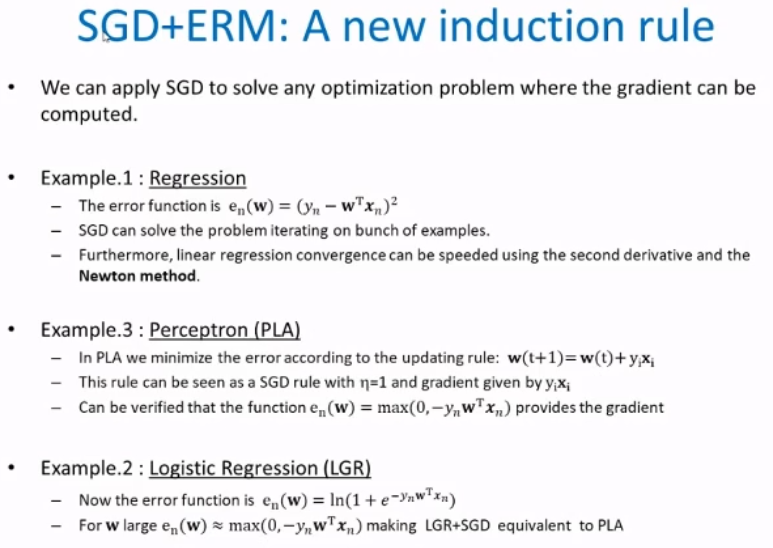
\includegraphics[width=0.8\textwidth]{images/sgd_erm}

	\end{figure}
	
	La función de pérdida o error $e$, debe ser adecuada a nuestro problema, las predicciones se basan en optimizarla, por tanto debe ser correcta para nuestro problema. Ejemplo:
	\begin{figure}[H]
		\centering
		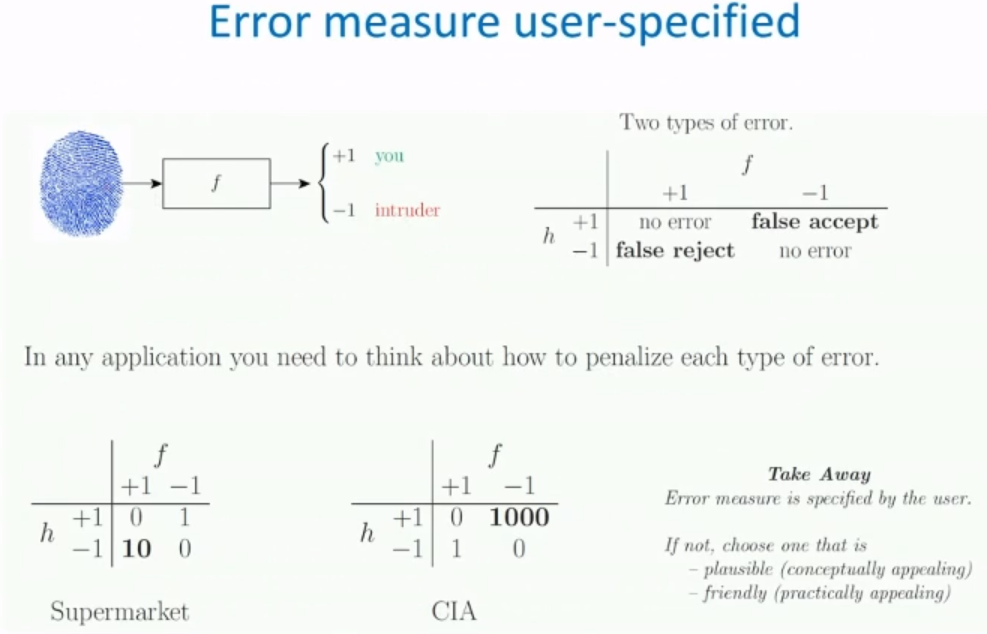
\includegraphics[width=0.8\textwidth]{images/fingerprint_example}

	\end{figure}
	
	\subsection{Añadiendo funciones a $\mathcal{H}$ (no lineales en $x$)}
	Hay ocasiones en las que ajustar linealmente con los valores del vector características extraído no es suficiente. 
	\begin{figure}[H]
		\centering
		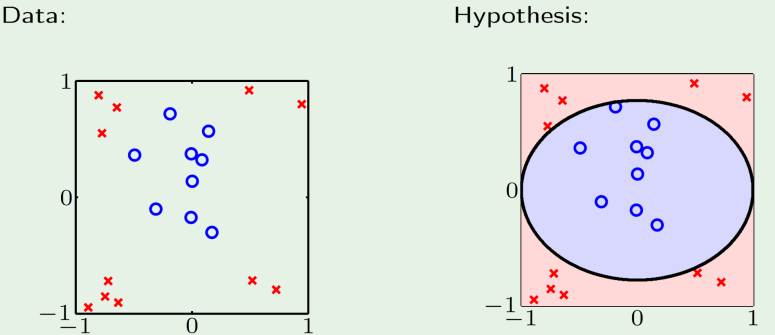
\includegraphics[width=0.8\textwidth]{images/linear_limited}
	\end{figure}
	¿Cómo hacer lo de la derecha? añadiendo a los valores $(x_1,\ldots,x_d)$ funciones no lineales de $x_1,\ldots,x_d$ (que ``aportan nueva información''), por ejemplo: polinomios, seno, coseno, tangente...
	
	Con $x$ nos referiremos al vector de características original, cuando ampliemos utilizaremos $z$, que tendrá a las $x$ y las añadidas.
	
	\begin{figure}[H]
		\centering
		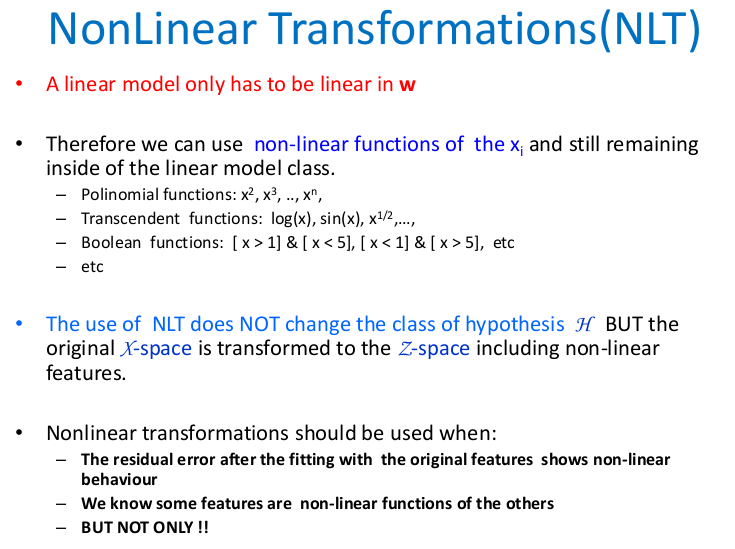
\includegraphics[width=0.68\textwidth]{images/nlt}
	\end{figure}
		
	\begin{figure}[H]
		\centering
		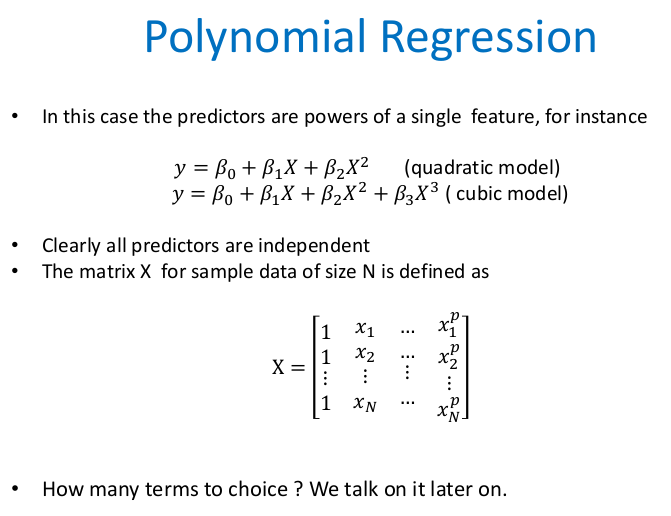
\includegraphics[width=0.68\textwidth]{images/pol_reg_notlin}
	\end{figure}
	
	Habrá que tener cuidado con cuántos términos se escogen pues el error fuera de la muestra estará acotado (clasificación) o será igual (regresión lineal) al error dentro de la muestra más un término que depende de la complejidad de las funciones. A la hora de escoger cuántos términos habrá que mantener un equilibrio entre la complejidad de las funciones y el error dentro de la muestra que conseguimos, esto nos determinará el error en la población, fuera de la muestra, que obtendremos.
	
	%\subsubsection{Non Linear Transformations}
	\begin{figure}[H]
		\centering
		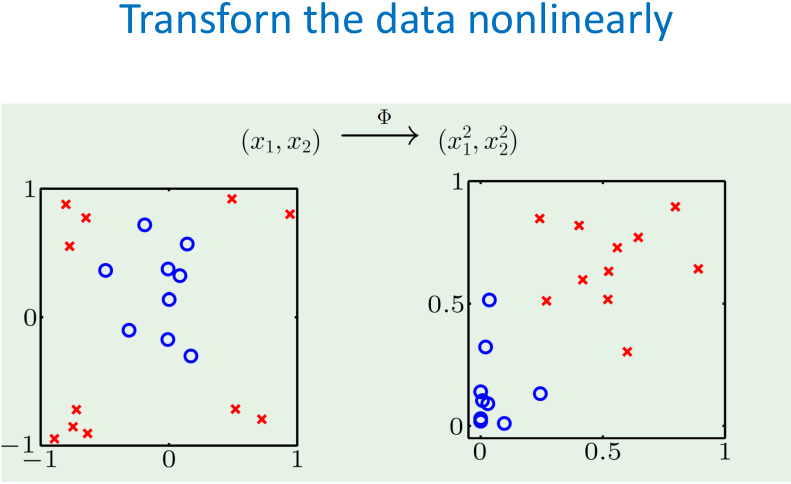
\includegraphics[width=0.65\textwidth]{images/transforn}
	\end{figure}
	
	\begin{figure}[H]
		\centering
		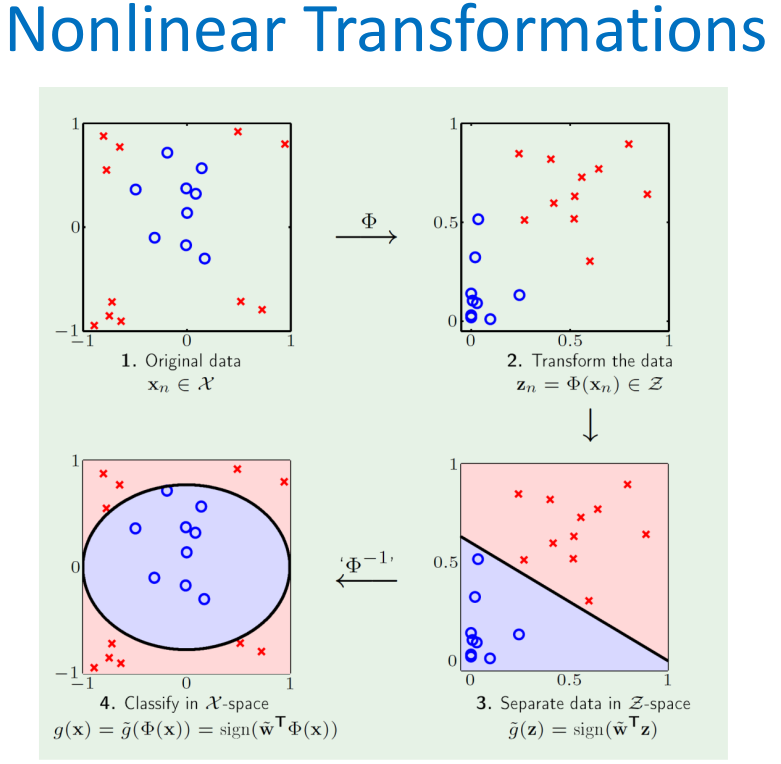
\includegraphics[width=0.7\textwidth]{images/nonlinear_transforn}
	\end{figure}
	Estas transformaciones para tener un mejor ajustes son interesantes pero hasta cierto punto. Estamos trabajando con una muestra concreta, si ajustamos muy bien una muestra concreta, pregunta ¿Qué pasará fuera de la muestra? (es muy posible que en nuevas muestras la función no funcione)
	
	\begin{figure}[H]
		\centering
		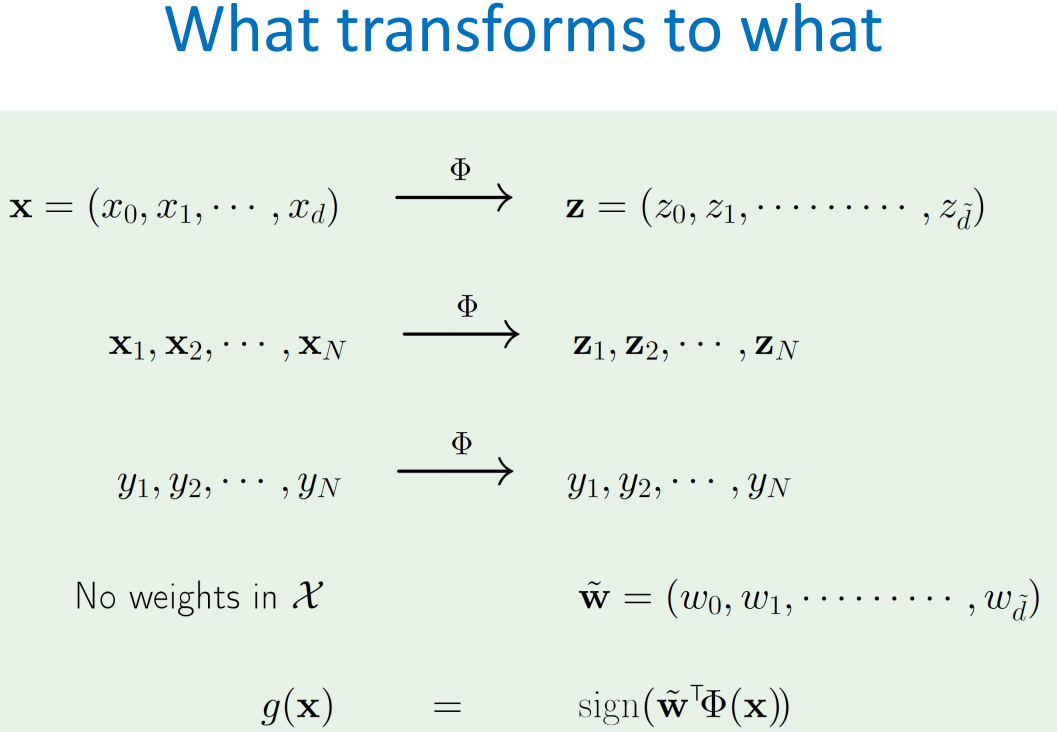
\includegraphics[width=0.6\textwidth]{images/what_trans_to_what}
	\end{figure}
	$\hat d >> d$, tendremos en $z$ a $x$ y las nuevas funciones hasta $\hat d$. Como ahora hay $\hat d$ elementos en $z$, tenemos que usar $\tilde w = (w_0,w_1,\ldots, w_{\hat d})$ y la complejidad para buscar en este espacio aumenta enormemente (recordar el caso de iteraciones para PLA \hyperlink{plaResult}{(PLA result)})
	
	\begin{figure}[H]
		\centering
		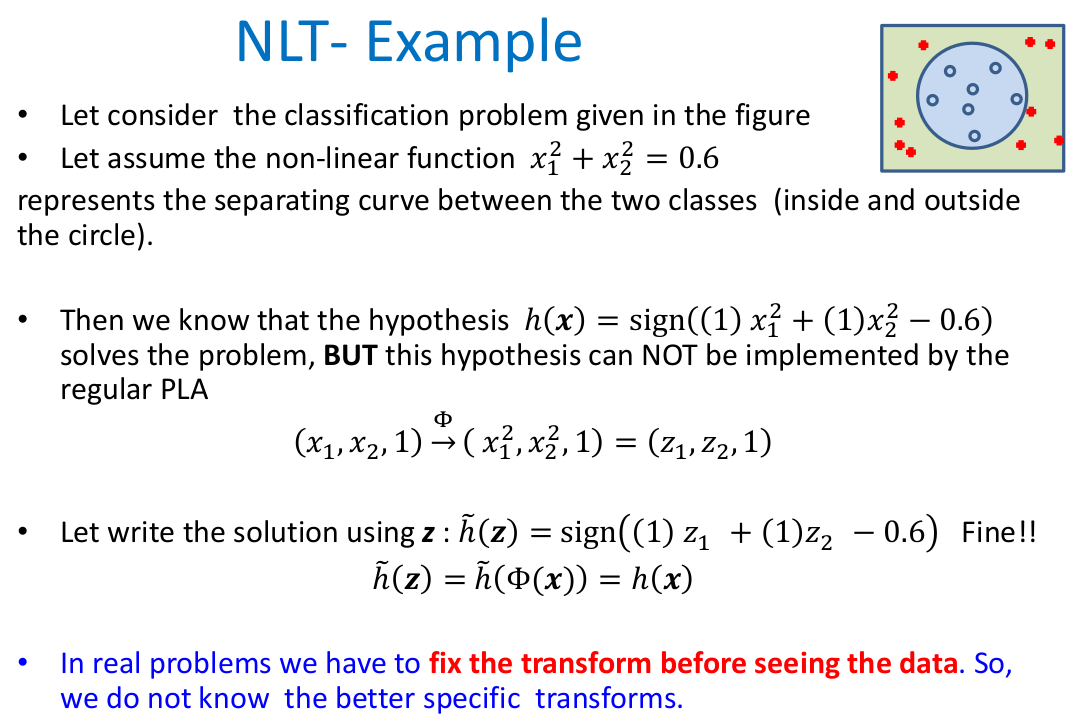
\includegraphics[width=0.65\textwidth]{images/nlt_example}
	\end{figure}
	
	Notación general
	\begin{figure}[H]
		\centering
		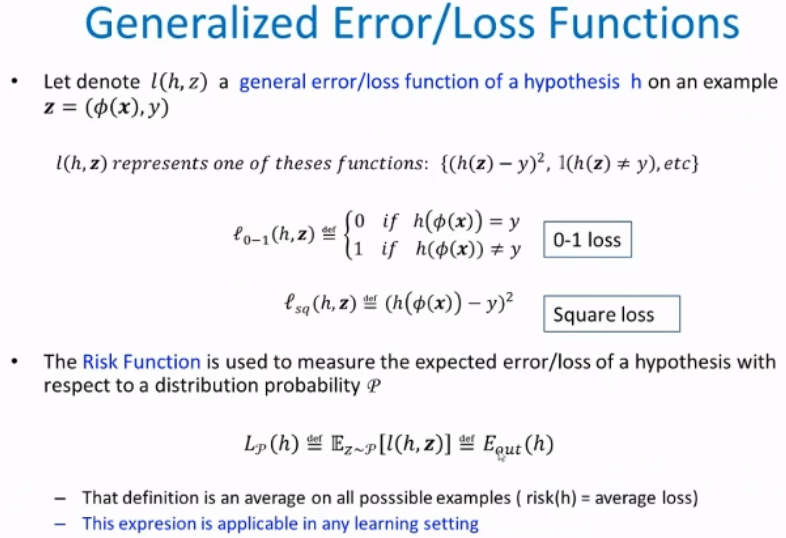
\includegraphics[width=0.65\textwidth]{images/notation_loss}
	\end{figure}
	
	\begin{figure}[H]
		\centering
		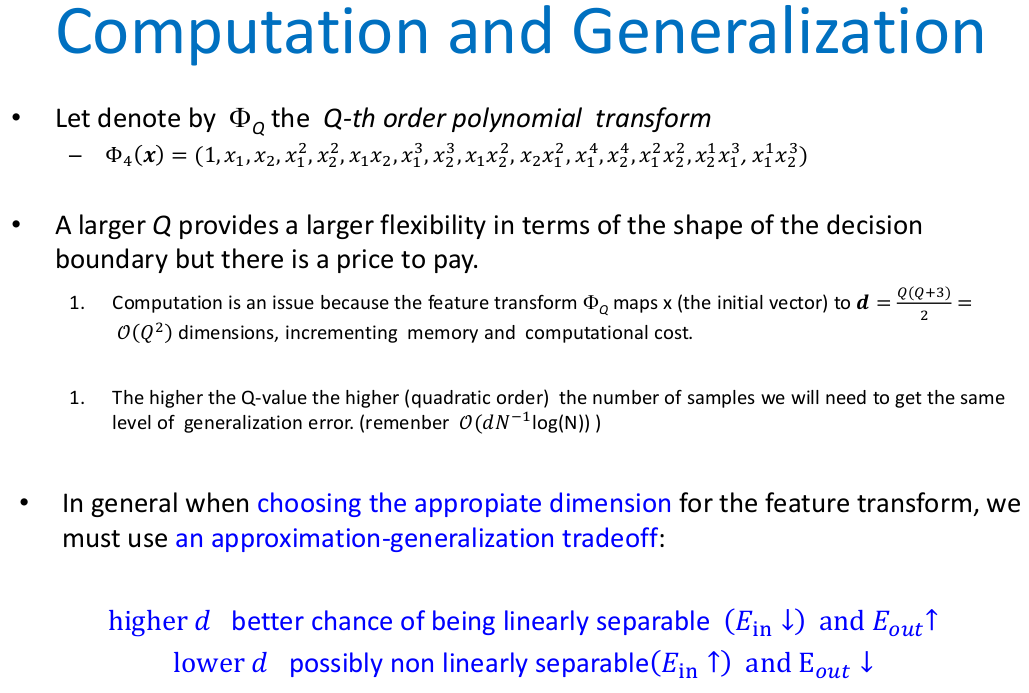
\includegraphics[width=0.65\textwidth]{images/q_pol_generalization}
	\end{figure}
	
	\subsection{Métricas de evaluación (para nuestros ajustes) - Clasificación}
	Vamos a ver métricas para evaluar los ajustes realizados mediante clasificación, mediante regresión está claro es el de menor error.
	
	En concreto clasificación binaria, para más dimensiones solo se utiliza matriz de confusion.
	
	Notación: TP=``true positives'', FP=``false positives'' (realmente son negativos), FN=``false negatives'' (realmente son positivos), TN=``True negatives''. Al igual que con las funciones de error, cuando clasificamos habrá medidas que nos interesen más que otras para el problema en el que nos encontremos.
	\begin{figure}[H]
		\centering
		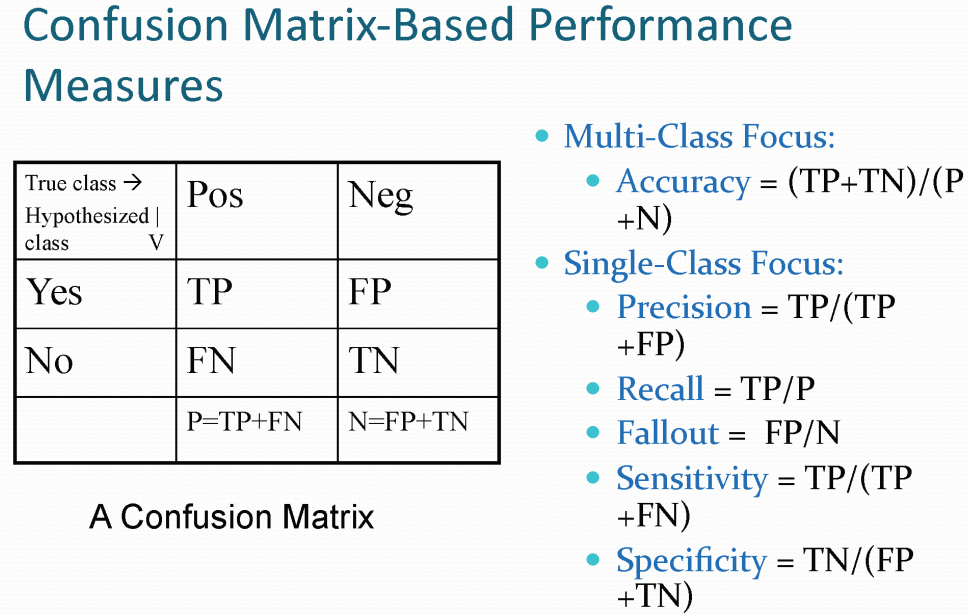
\includegraphics[width=0.64\textwidth]{images/confusion_matrix}
	\end{figure}
	Multi-Class
	\begin{itemize}
		\item Accuracy: total de aciertos en positivos y negativos entre el total de positivos y negativos
	\end{itemize}
	Single-Class
	\begin{itemize}
		\item Sensitivity: proporción de verdaderos casos positivos que el algoritmo ha sido capaz de detectar
		\item Specifity: igual que anterior, es el número de negativos acertados en proporción al total de casos negativos que existen
		\item Precision: proporcion de positivos entre el número que el algoritmo ha detectado como positivos
	\end{itemize}

	
	\begin{figure}[H]
		\centering
		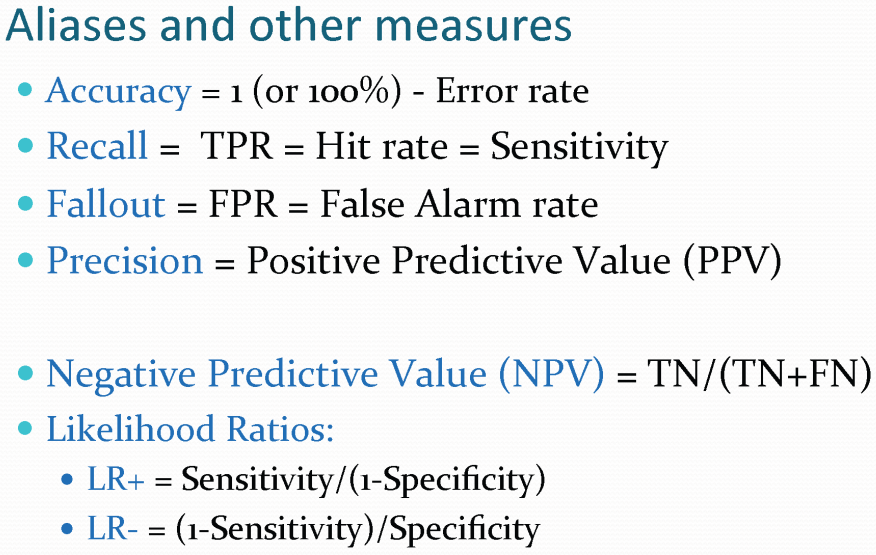
\includegraphics[width=0.6\textwidth]{images/aliases_other_measures}
	\end{figure}
	
	\begin{figure}[H]
		\centering
		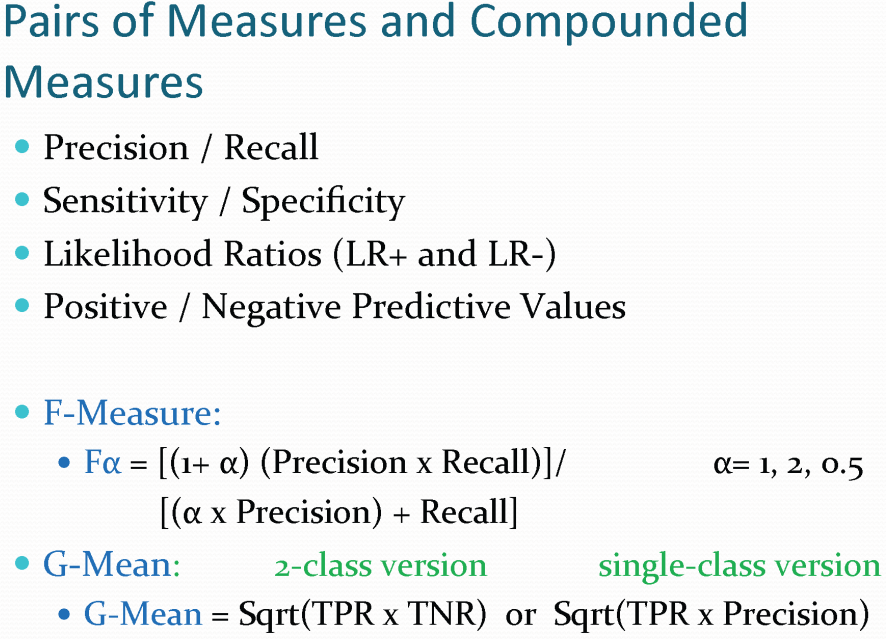
\includegraphics[width=0.6\textwidth]{images/f_measure}
	\end{figure}
	F-medida es importante. Cuando se minimiza se intenta buscar minimizar las dos colas a la vez. Si no se tiene predilección por un error u otro, lo que hay que intentar es encontrar una medida que haga mínima las dos colas. La F-medida es el índice más standard que existe en problemas de clasificación general.
	
	\textbf{Otra medida importante}\\
	Podemos plantearnos ¿Cómo de bueno es un clasificador frente a un clasificador aleatorio?
	
	\begin{figure}[H]
		\centering
		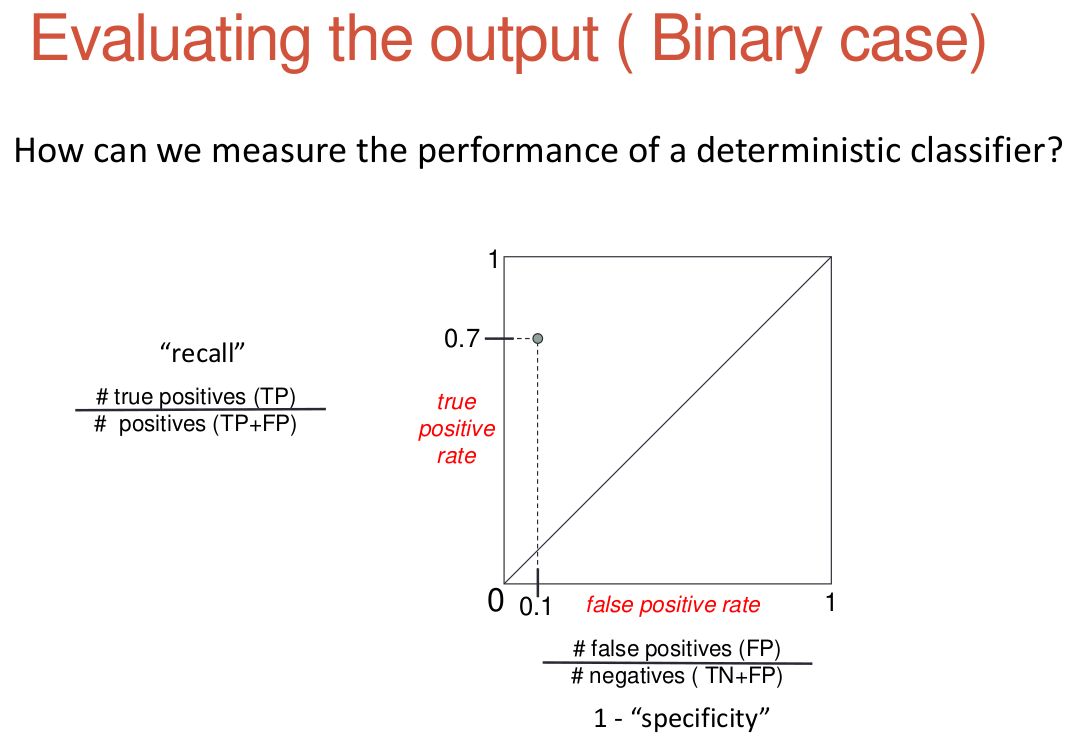
\includegraphics[width=0.6\textwidth]{images/eval_output_deter}
	\end{figure}
	Para tener 0.7 de proporción de true positive rate, hemos tenido que tragarnos un 0.1 de false positive rate. Lo ideal sería línea horizontal en 1.\\
	
	Caso de regresión logística. Ahora, en el caso de clasificador probabilístico podríamos asignar la clase con más probabilidad, pero también podríamos a partir de 0.6 asignar a una clase y por debajo a la otra, o a partir de 0.4; son otras formas de clasificar.\\
	Cuando tenemos un clasificador probabilístico podemos construir lo que se denomina la curva ROC. La curva ROC es la curva que nos va diciendo, para cada valor de incremento de falsos positivos, cómo evoluciona el clasificador en términos de cada vez ir mejorando. Si se le permite al clasificador tragarse todos los errores que sea $\Rightarrow$ también acertará mucho.
	
	\begin{figure}[H]
		\centering
		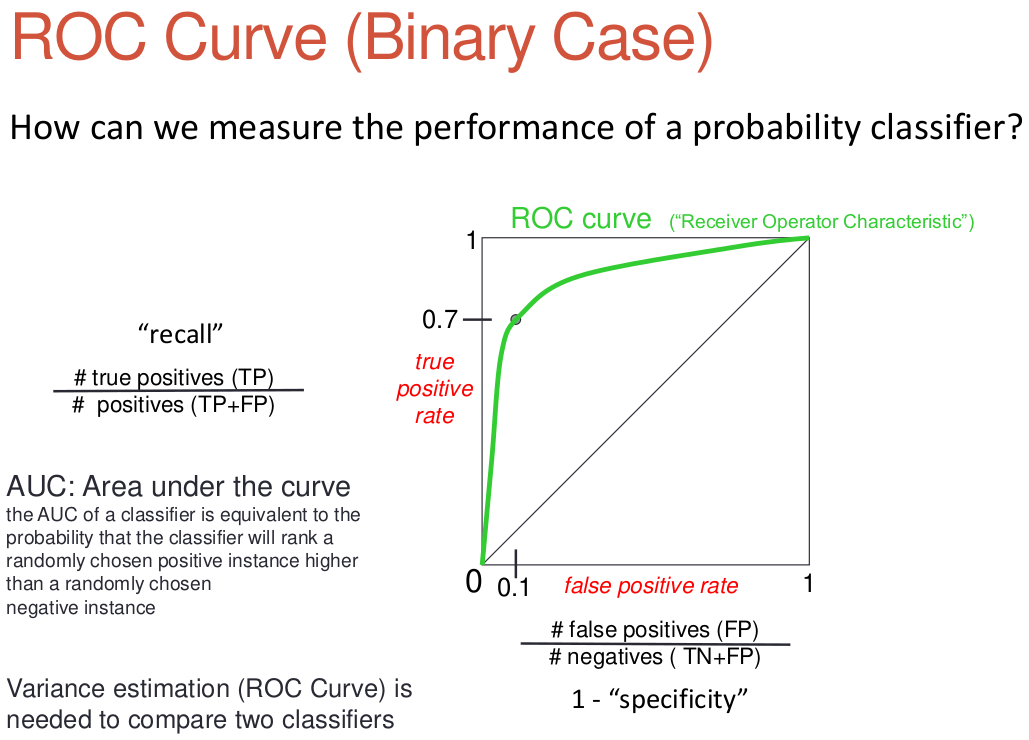
\includegraphics[width=0.7\textwidth]{images/roc_curve}
	\end{figure}
	En la línea gris se representa si la curva de clasificador que asigna 50\% y 50\%. Podemos ver cuánto se separa la curva verde del clasificador 50\%, 50\%. El área bajo la curva es la media de éxito del clasificador si promedias cualquier decisión que se tome para poder realizar la clasificación. Si la curva sube mucho el área estará muy próxima a 1 y tendremos un magnífico clasificador, porque en cada circunstancia es capaz de acertar bien. Si la curva se acerca a la línea gris entonces estamos cerca de hacerlo aleatorio
	
	El área de curva ROC y el propio dibujo de la curva nos permite comparar clasificadores muy bien independientemente del criterio usado para la clasificación. En la curva ROC están representados todos los posibles criterios. Esta curva tiene todos los criterios y podemos comparar cualesquiera dos clasificadores sin ningún tipo de problema.
	
	\textit{Nota:} estas curvas están ligadas a una muestra concreta, si tomamos otra muestra es posible que las curvas ROC cambien. Así que hacerlo bien sería calcular curva ROC con algún tipo de media más varianza en cada punto. Es raro ver estas estimaciones, pero la gente que lo hace bien evidentemente que la pone. La curva ROC es la media de un comportamiento. No es lo mismo una curva ROC con desviación típica muy pequeña que una curva ROC que puede oscilar muchísimo.
	
	La curva ROC es el criterio más normal que utilizaremos para comparar los resultados de nuestros clasificadores binarios.
	
	\begin{figure}[H]
		\centering
		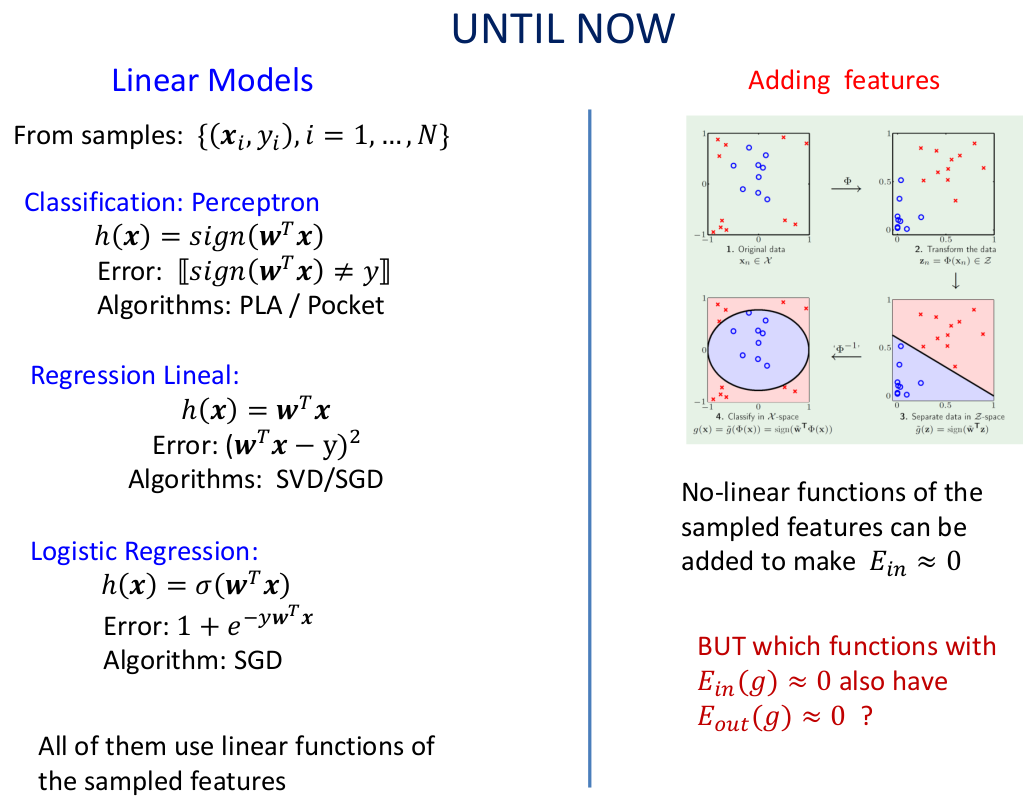
\includegraphics[width=0.7\textwidth]{images/until_now}
	\end{figure}
	\newpage
	
	\section{Fundamental of Learning (ERM rule)}
	El aprendizaje que estamos viendo y seguiremos viendo es aprendizaje estadístico. Está basado en lo que se llama aprendizaje inductivo, es decir, extraer información de una muestra y llevarla al total de la población. ¿En qué condiciones eso puede darnos resultado?
	
	Veamos dos ejemplos de aprendizaje inductivo determinísticos
	
	\begin{figure}[H]
		\centering
		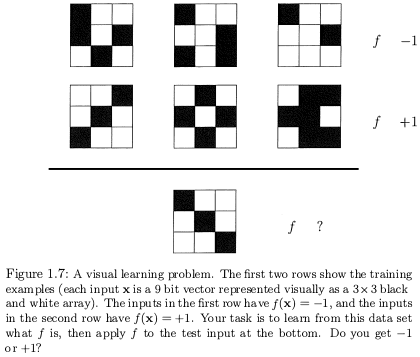
\includegraphics[width=0.6\textwidth]{images/learning_not_feasible1}
	\end{figure}
	Supongamos que tenemos una muestra de 5 elementos
	\begin{figure}[H]
		\centering
		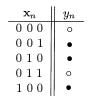
\includegraphics[width=0.15\textwidth]{images/learning_not_feasible2}
	\end{figure}
	
	Al ser finito, podemos describir los elementos de la población restantes junto con las 8 posibilidades para la función $f$.
	\begin{figure}[H]
		\centering
		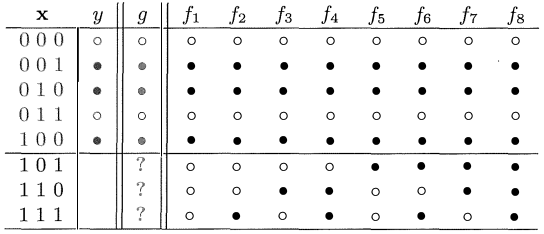
\includegraphics[width=0.5\textwidth]{images/learning_not_feasible3}
	\end{figure}
	
	Cualquiera de las $f_i$, $i\in \{1,\ldots,8\}$ candidatas a $f$ es válida. Es decir, no podemos conocer $f$ fuera de la muestra conociendo los valores de $f$ solo en una muestra. No podemos conocer $f$ fuera de $\mathcal{D}$
	
	En tanto que no se conoce $f$, conocer $\mathcal{D}$ no nos sirve para deducir patrones de $f$ fuera de $\mathcal{D}$. Por tanto las predicciones de $g$ fuera de $\mathcal{D}$ no sirven.
	
	Podremos aprender aún desconociendo $f$ haciendo uso de la función de probabilidad. En este caso aprenderemos menos, no estaremos seguros. En ese caso sí es posible, a partir de una muestra, obtener información de la población. Pero nunca es información determinista.\\
	
	\textbf{Nueva hipótesis:} los elementos de la muestra $\mathcal{D}$ son muestras iid de una distribución de probabilidad $P$. Habrá veces que no sean iid en la práctica, al ser métodos robustos puede que funcione igual; pero siempre hay que intentar satisfacer las hipótesis.
	
	Desde este momento se extrae un trozo de la población. Pregunta: ¿Es representativo ese trozo de la población?
	\begin{itemize}
	\item Probabilísticamente hablando si lo hemos hecho bien podría ser (probabilísticamente quiere decir que si yo sacara muchas muestras con ese sistema, la media de los resultados de todas esas muestras cuadra; pero nosotros tomamos una sola muestra y si tenemos mala suerte nos sale una muestra de las colas de la distribución y no es representativa de la distribución); pero no es algo que represente a la información. 
	
	La verdadera solución no sería la que yo extraigo de una muestra concreta que he sacado; sería la media de las soluciones de muchas muestras. Podríamos decir entonces la solución media con su desviación típica. Eso sí se parecería bastante a la solución de la población.
	
	Como hacer esto es inviable, hay que suponer que hemos tomado muestra representativa de la población. ¿Cuándo podemos pensar que es suficientemente representativa de la población?, tomando $N\to \infty$
	\item  determinísticamente bajo ningún concepto.
	
	\end{itemize}
	
	\begin{figure}[H]
		\centering
		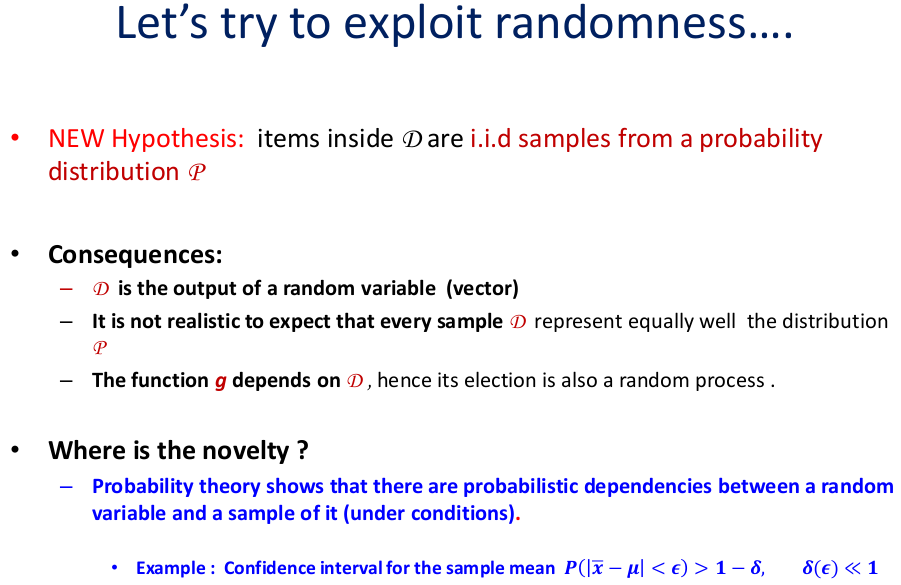
\includegraphics[width=0.7\textwidth]{images/randomness}
	\end{figure}
	((últimas líneas) $\sim$ Lo que conseguimos es poder aplicar la Ley Fuerte de los Grandes números: si tenemos $X_1,X_2,X_3,\ldots$ una sucesión infinita de v.a. iid con $E(|X_i|)<\infty$ y tienen valor esperado $\mu$, entonces $P(\lim_{n\to \infty} \overline{X_n} = \mu ) =1$)
	
	\begin{figure}[H]
		\centering
		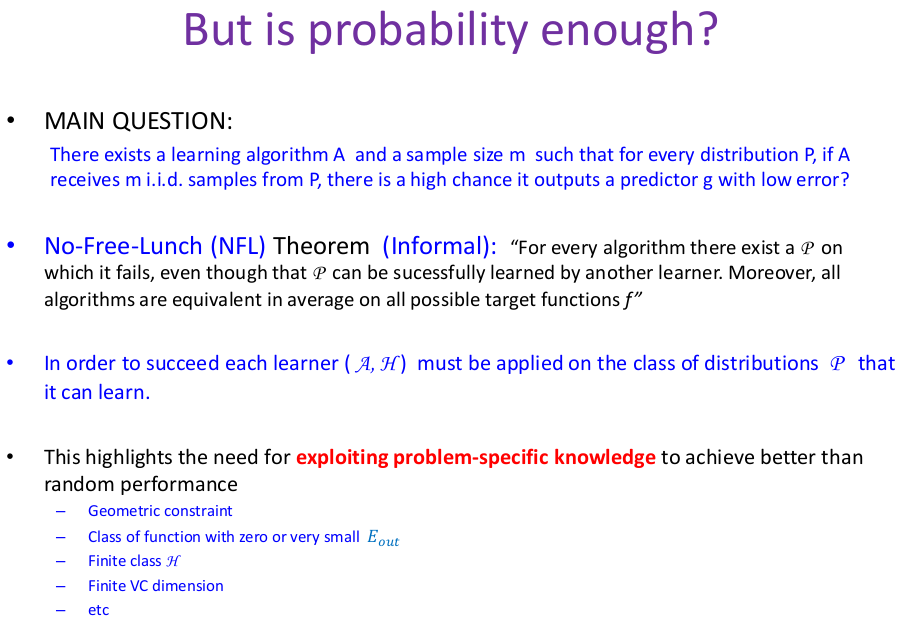
\includegraphics[width=0.7\textwidth]{images/prob_not_enough}
	\end{figure}
	\textit{Nota:} en principio necesitamos definir $\mathcal{H}$ previamente para poder aprender, debemos elegir una clase que se intuya que puede ser buena para el problema. No-Free-Lunch viene a decir que no hay algoritmo universal que sirva para todos los problemas. Además el éxito medio para todos los problemas que pudieran existir, el éxito medio es común para todos
	
	
	\subsection{¿Can we infer something outside $\mathcal{D}$ using only $\mathcal{D}$? - The PAC answer}
	Ejemplo: tenemos bolas rojas y verdes en un contenedor...
	\begin{figure}[H]
		\centering
		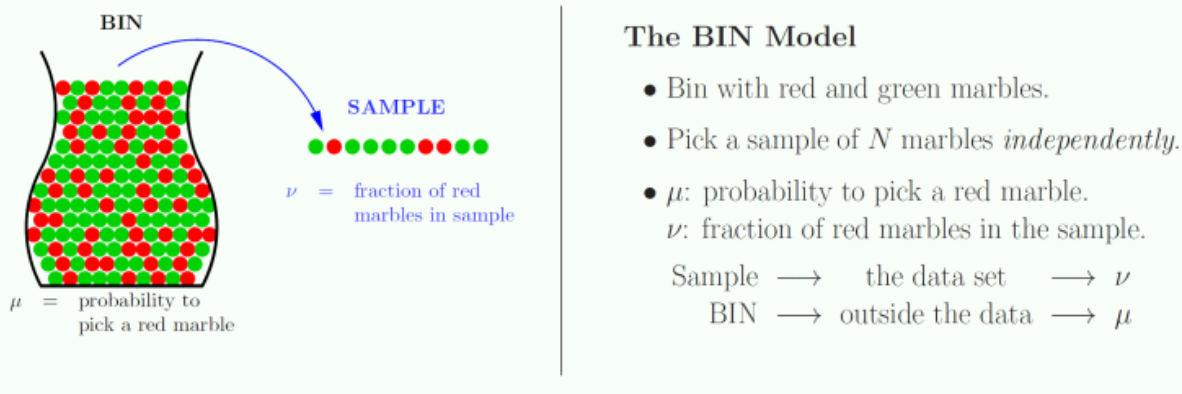
\includegraphics[width=0.8\textwidth]{images/marbles}
	\end{figure}
	
	\begin{itemize}
		\item ¿Podemos garantizar algo sobre $\mu$ (fuera de la muestra) después de observar $\upnu$ (dentro de la muestra)? - No, podríamos haber obtenido una muestra donde todas las bolas son verdes cuando el contenedor tiene en su mayoría bolas rojas.
		\item ¿Por qué se confía o realizan entonces métodos como las encuestas? - Porque el caso malo es posible pero no probable. Además cuando $N\to \infty$ tenemos $\upnu \to \mu$
	\end{itemize}
	
	Hoeffding/Chernoff probó que, most of the time, para un $\mu$ fijo, $\upnu$ no puede estar muy lejos de $\mu$
	\begin{proposition}[\bf Desigualdad de Hoeffding]
	$$P(\mathcal{D}:\ |\mu - \upnu| >\epsilon) \leq 2 e^{-2\varepsilon ^2 N} \quad \forall \epsilon >0$$
	$$P(\mathcal{D}:\ |\mu - \upnu| \leq \epsilon) \geq 1 - 2e^{-2\epsilon^2 N} \quad \forall \epsilon > 0$$
	donde $\upnu$ es v.a. . Traducción (Hoeffding inequality)\\
	Sean $(X_1, \ldots,  X_N)$ una m.a.s. (iid), acotadas en intervalo $[0,1]$, $0\leq X_i\leq 1$
	$$P(|\overline{X} - E[\overline{X}]| \geq \epsilon) \leq 2e^{-2N\epsilon^2} \quad \forall \epsilon >0$$
	Para nuestro caso se toma m.a.s. de v.a. $X\sim Bernoulli(\mu)$, la realización de $\overline{X}$ es $\upnu$ y $E[\overline{X}]=\frac{1}{N} \sum_{i=1}^N E[X_i]=\frac{nE[X]}{n}=\frac{n\mu}{n}=\mu$
	
	\end{proposition}
	
	\begin{figure}[H]
		\centering
		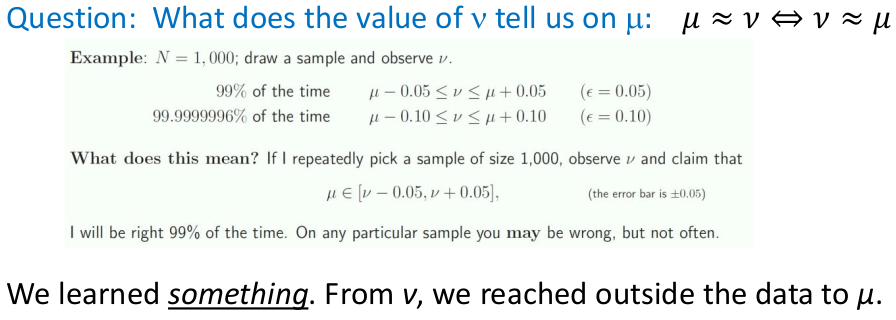
\includegraphics[width=0.83\textwidth]{images/hoeffding_learned_something}
	\end{figure}
	
	\begin{figure}[H]
		\centering
		\includegraphics[width=0.73\textwidth]{images/hoeffding_remarkable}
	\end{figure}
	
	¿Cómo se relaciona el modelo del contenedor con el problema de aprendizaje? Parece que lo desconocido era solo $\mu$ cuando en aprendizaje es la función $f\colon \mathcal{X} \to \mathcal{Y}$. Tomar una hipótesis $h\in \mathcal{H}$ y comparar $h$ con $f$ en cada $x\in \mathcal{X}$. Si $h(x)=f(x)$, colorear $x$ en verde. Si $h(x)\neq f(x)$ colorear punto $x$ en rojo. Si tomamos $x$ aleatoriamente de acuerdo a una distribución de probabilidad $P$ en el espacio de entrada $\mathcal{X}$, sabemos que $x$ tendrá una probabilidad, $\mu$, de ser rojo y una probabilidad, $1-\mu$ de ser verde. Ahora $\mathcal{X}$ se comporta como el contenedor del ejemplo.
	
	\textit{Nota:} yo veo que añadimos vector aleatorio $z=(z_1,\ldots, z_N)\colon  \R^{d+1}\supset \mathcal{D} \to \R$ de Bernoulli $z_n=[[h(x_n)\neq f(x_n)]]$, contamos los fallos, las bolas rojas. Se aplica Hoeffding a $(z_1,\ldots, z_n)$, la probabilidad par esperanza y la $P$ serán las de esp probabilístico $(\R^{d+1}, \mathcal{B}(\R^{d+1}), P_\mathcal{D})$, viendo $\mathcal{D}$ como vector aleatorio.
	
	Con esto, ya se puede aplicar la desigualdad de Hoeffding al problema de aprendizaje, permitiéndonos aprender fuera de $\mathcal{D}$. Usando $\upnu$ para predecir $\mu$ conseguimos saber algo sobre $f$ aunque no nos determina $f$. Lo que nos dice $\mu$ es el error que $h$ comete al aproximar $f$. Si $\upnu$ es cercana a 0, podemos predecir que $h$ va a aproximar a $f$ bien sobre todo el espacio de entrada $\mathcal{X}$.\\
	$\upnu$ está asociado a $h$. En aprendizaje buscaremos la mejor $h\in \mathcal{H}$ que nos de una baja tasa de error.\\
	
	\textit{Notación:} introduciremos nombres más descriptivos para los componentes que vamos a usar
	$$E_{in}(h) = \text{(fracción de } \mathcal{D} \text{ donde } f \text{ y } h \text{ no coinciden)}=\frac{1}{N} \sum_{n=1}^N [[h(x_n) \neq f(x_n)]]$$
	también definimos el error fuera de la muestra ($P(z=1)$)
	$$E_{out}(h)=P[h(x)\neq f(x)]$$
	que corresponde a $\mu$ en el modelo del contenedor. La probabilidad está basada en la distribución $P$ sobre $\mathcal{X}$ usada para tomar los puntos muestrales $x$. 
	
	
	\begin{figure}[H]
		\centering
		\includegraphics[width=0.73\textwidth]{images/bin_model_and_learning}
	\end{figure}
	
	Con la nueva notación, \underline{fijado un $h\in \mathcal{H}$} y sustituyendo $\upnu$ por $E_{in}(h)$ y  $\mu$ por $E_{out}(h)$ la desigualdad de Hoeffding puede reescribirse
	$$P[\mathcal{D}:\ |E_{in}(h)-E_{out}(h)|>\epsilon]\leq 2e^{-2\epsilon ^2N} \quad \forall \epsilon >0$$
	This is called a \textbf{``Probably Approximately Correct (PAC)''}
	
	\begin{figure}[H]
		\centering
		\includegraphics[width=0.73\textwidth]{images/hoeffding_says}
	\end{figure}
	
	\begin{enumerate}
		\item Si $E_{in}(h)=1$ entonces el complementario de $h$, $\hat h$ tendrá $E_{in}(\hat h)=0$
		\item $E_{in}(h)=1$ o uno con una muestra muy pequeña
	\end{enumerate}
	
	
	\begin{figure}[H]
		\centering
		\includegraphics[width=0.73\textwidth]{images/understanding_pac_results}
	\end{figure}

	Consideremos ahora un conjunto hipótesis $\mathcal{H}$ vez de una sola función hipótesis $h$, y asumimos que $\mathcal{H}$ tiene un número finito de hipótesis
	$$\mathcal{H}=\{h_1,h_2,\ldots ,h_M\}$$
	(aún se pueden representar con $M$ contenedores y $h_1,\ldots, h_M$, cada contenedor representando el espacio $\mathcal{X}$). Antes teníamos 
	$$P[\mathcal{D}:\ |E_{in}(h)-E_{out}(h)| > \epsilon ] \leq 2e^{-2\epsilon ^2 N} \quad \forall \epsilon >0$$
	para un $h$ ya fijado. Con múltiples hipótesis en $\mathcal{H}$, el algoritmo de aprendizaje elige una hipótesis final basado en $\mathcal{D}$. Nos gustaría obtener
	$$P[\mathcal{D}:\ |E_{in}(g)-E_{out}(g)|>\epsilon] \leq 2e^{-2\varepsilon ^2 N} \quad \forall \epsilon >0$$
	La hipótesis $g$ no está fijada previa a generar los datos, porque la hipótesis $g$ que se elige depende de los datos. Así que no podemos poner directamente $g$ en vez de $h$ en la desigualdad de Hoeffding (no sabemos cual es $g$ ?).
	
	$$[|E_{in}(g)-E_{out}(g)|>\epsilon] \subset \bigcup_{h_i\in H} [|E_{in}(h_i)-E_{out}(h_i)|>\epsilon]$$
	
	\begin{figure}[H]
		\centering
		\includegraphics[width=0.73\textwidth]{images/then_what}
	\end{figure}
	
	\begin{figure}[H]
		\centering
		\includegraphics[width=0.73\textwidth]{images/interpreting_bound}
	\end{figure}
	La cota de error o ``error bound'' $\sqrt{\frac{1}{2N} \ln \frac{2|\mathcal{H}|}{\delta}}$ depende de $|\mathcal{H}|$. Si $\mathcal{H}$ es infinito la cota diverge y no tiene sentido. Desafortunadamente casi todos los modelos de aprendizaje usan $\mathcal{H}$ infinito.
	....
	\subsection{Theory of Generalization}
	
	\subsubsection{Effective Number of Hypotheses}
	\newpage

	\section{Sobreajuste y Regularización.}	
	... Vamos a ver cómo usar la teoría de sesgo-varianza o dimensión VC para elegir realmente un buen modelo. Vamos a ver las técnicas que nos permiten elegir bien. Vamos a detectar cuales son los problemas que los datos nos presentan.
	
	Sobreajuste: realmente es mala elección del modelo.
	
	Nunca sabremos si el modelo es el correcto. Si tenemos muestra muy grande podemos tener mucha carga o evidencia de que el modelo puede ir bien en general.
	
	Ante el problema estamos restringidos a elegir una clase de funciones, la que se considere adecuada y correcta, y ajustar lo mejor posible dentro de esa clase de funciones. Cuando hacemos eso, por el compromiso sesgo-varianza, la elección de la clase de funciones puede dar un sesgo. Si se decide tomar clase de funciones enormemente grande, entonces podemos tener un problema de varianza. Podemos empezar a ajustar nuestros datos con fuciones que tienen tanta variabilidad que serían capaces de ajustar todos y cada uno de los datos, lo cual nos lleva a error.\\
	
	Entonces... ¿Cómo abordar esa problemática sesgo-varianza sin conocer la función verdadera? De ninguna forma. Vamos a ver cual es la filosofía de abordar el problema que más nos conviene. Lo único que nos puede llevar hacia adelante es una buena técnica.
	
	\begin{definition}[\textbf{Sobreajuste}]
	Un ``proceso'' se dice que sobreajusta dataset cuando al elegir $h$ con menor $E_{in}$ implica mayor $E_{out}$
	\end{definition}
	
	\textit{Nota:} Suele  traducirse en bajo error en entrenamiento y alto error en test.
	
	De acuerdo con la cota VC, $E_{out}(g)\leq E_{in}(g)+\Omega (N,\mathcal{H},\delta)$ donde la función de penalización, $\Omega$, incrementa muy rápido con la dimensión VC.\\
	
	¿Por qué ocurre esto?
	
	\begin{itemize}
		\item Error estocástico: etiquetado ruidoso. En este caso se necesitarían funciones más complejas para obtener menor error en la muestra.
		\item Error determinístico: ruido del modelo. La complejidad de la verdadera función no está bien representada por el vector de características (hay variables aleatorias implicadas en $f$ no consideradas).
	\end{itemize}
	 
	 Usualmente el sobreajuste ocurre cuando nuestro modelo explica los datos de entrenamiento demasiado bien. En general no es fácil detectar el sobreajuste ya que también depende de entidades desconocidas (ruido en los datos).
	\begin{figure}[H]
		\centering
		\includegraphics[width=0.7\textwidth]{images/overfitting_example}
	\end{figure}
	
	Con polinomio de orden 9 conseguimos error 0 en la muestra. Pero, si se cambia un poco los datos, y se elige de nuevo polinomio de orden 9 ajustaríamos de nuevo con error 0, pero este segundo polinomio sería muy distinto al primero. Este es el concepto de varianza enorme. En cuanto se mueve la muestra lo más mínimo, la función que explica la muestra cambia enormemente. No parece que se esté modelando un fenómeno, si los datos cambian un poco la función debería cambiar un poco.
	
	La mayoría de la veces el sobreajuste es consecuencia de considerar $\mathcal{H}$ más compleja de lo requerido... aunque no siempre.\\
	
	¿Cómo evitar sobreajuste? ¿Cómo elegir la complejidad correcta de la solución?
	\begin{itemize}
		\item \textbf{Solución 1:} Restringir la clase de funciones $\mathcal{H}$ (por ejemplo pasar de polinomios de orden 3 a polinomios de orden 2.\\
		Esta técnica se llama \textbf{sesgo inductivo}
		\item \textbf{Solución 2:} Imponer condiciones adicionales en la función de error (ajustar pesos para evitar zonas no acordes como en el ejemplo de polinomio de orden 9 anterior; de todos los polinomios de orden 9 me quedo con los que tengan $w$ que no acentúen mucho los errores como las curvas en ejemplo anterior).\\
		Se permite clase de funciones con mucha variabilidad pero luego voy a tratar de restringir los elementos de dicha clase tanto como se pueda de acuerdo al problema que se tenga.
		Esta técnica se llama \textbf{regularización}.
	\end{itemize}
	
	\begin{figure}[H]
		\centering
		\includegraphics[width=0.8\textwidth]{images/overfitting_example2}
	\end{figure}
	
	\textbf{Caso de estudio:}\\
	Consideremos dos ejemplos, con función objetivo y dataset, de regresión:
	
	\begin{figure}[H]
		\centering
		\begin{subfigure}{.5\textwidth}
  		\centering
  		\includegraphics[width=0.8\textwidth]{images/with_added_noise}
  		\caption{Con ruido.}
  		\label{fig:sub1}
		\end{subfigure}%
		\begin{subfigure}{.5\textwidth}
  		\centering
  		\includegraphics[width=0.8\textwidth]{images/noiseless}
  		\caption{Función objetivo compleja sin ruido.}
  		\label{fig:sub2}
		\end{subfigure}
		\caption{}
		\label{fig:test}
	\end{figure}
	
	No podemos distinguir cuando hay o no ruido ni el origen.\\
	
	¿Cuál sería el mejor ajuste?\\
	
	Probemos en ambos casos polinomio de orden 2 y polinomio de orden 10.
	
	\begin{figure}[H]
		\centering
		\begin{subfigure}{.5\textwidth}
  		\centering
  		\includegraphics[width=0.8\textwidth]{images/case_study1}
  		\caption{Con ruido.}
  		\label{fig:sub1}
		\end{subfigure}%
		\begin{subfigure}{.5\textwidth}
  		\centering
  		\includegraphics[width=0.8\textwidth]{images/case_study2}
  		\caption{Función objetivo compleja sin ruido.}
  		\label{fig:sub2}
		\end{subfigure}
		\caption{En ambos casos se obtiene mejor resultado, menor ruido $E_{out}$ en el caso de polinomio de bajo grado.}
		\label{fig:test}
	\end{figure}
	\textit{Nota:} El tamaño de la muestra es más representativo para primer caso que segundo, pero no es representativo para ninguno de los dos casos; si tuviésemos muestra más grande, es posible que tuviésemos comportamiento al revés.
	\textit{Nota:} Tenemos que tener más muestras en función de la función $f$ que tengamos, aunque nunca sabemos cual es la función $f$. El número de muestras nos dice como de complicado podemos llegar en el mejor de los casos.
	
	\begin{figure}[H]
		\centering
		\begin{subfigure}{.5\textwidth}
  		\centering
  		\includegraphics[width=0.8\textwidth]{images/stochastic_noise}
  		\caption{Ruido estocástico: ruido aleatorio i.i.d. añadido a los datos}
  		\label{fig:sub1}
		\end{subfigure}%
		\begin{subfigure}{.5\textwidth}
  		\centering
  		\includegraphics[width=0.8\textwidth]{images/deterministic_noise}
  		\caption{Ruido determinístico: la parte de la función objetivo fuera del mejor ajuste $\overline{g}$\\ Este ruido depende de $\mathcal{H}$}
  		\label{fig:sub2}
		\end{subfigure}
		\caption{}
		\label{fig:test}
	\end{figure}
	$$y=g_{\mathcal{D}}^*(x)+noise, \quad \quad noise = stochastic\ noise + deterministic\ noise$$
	Dado un dataset $\mathcal{D}$ y $\mathcal{H}$ fijados, no podemos distinguir entre ambos tipos de ruido.
	$$E_{\mathcal{D}}[E_{out}(g^{(\mathcal{D})})]=\sigma ^2 + bias + var = stochastic\ noise + deterministic\ noise + var$$
	Dado que $\sigma^2$ es el que pertenece a las oscilaciones de ruido estocástico y no podemos hacer nada con él. Entonces sesgo y varianza son las dos cosas que se pueden atacar. Hay que adquirir un compromiso.	Hay que reducir la parte que de más ruido. Qué da más ruido sesgo o varianza?
	
	Para el ejemplo anterior
	
	\begin{figure}[H]
		\centering
		\begin{subfigure}{.5\textwidth}
  		\centering
  		\includegraphics[width=0.8\textwidth]{images/learning_curve1}
  		\caption{Polinomio de orden 2}
  		\label{fig:sub1}
		\end{subfigure}%
		\begin{subfigure}{.5\textwidth}
  		\centering
  		\includegraphics[width=0.8\textwidth]{images/learning_curve2}
  		\caption{Polinomio de orden 10}
  		\label{fig:sub2}
		\end{subfigure}
		\caption{}
		\label{fig:test}
	\end{figure}
	Para el polinomio de orden 2 la zona gris es un ajuste razonable. En cambio para polinomio de orden 10 no lo es. Hasta que no se llega a una cantidad, digamos 10, de puntos hay sobreajuste (pasa por todos ellos); el $E_{out}$ en la zona gris es enorme. A partir de zona gris, en polinomio de orden 10 ya no se puede decir que haya sobreajuste.
	
	\textit{Nota:} la complejidad de la función es importante para que no haya sobreajuste pero no es por sí sola, es en relación al tamaño de la muestra que tenemos
	\section{Regularización: a smart mechanism to implement SRM}
	La idea de regularización es restringir el modelo de aprendizaje para mejorar el error fuera de la muestra
	\begin{figure}[H]
		\centering
		\begin{subfigure}{.5\textwidth}
  		\centering
  		\includegraphics[width=0.8\textwidth]{images/free_fit}
  		\caption{Free fit}
  		\label{fig:sub1}
		\end{subfigure}%
		\begin{subfigure}{.5\textwidth}
  		\centering
  		\includegraphics[width=0.8\textwidth]{images/restrained_fit}
  		\caption{Restrained fit}
  		\label{fig:sub2}
		\end{subfigure}
		\caption{Las figuras muestran la dramática mejora en el ajuste con una pequeña cantidad de regularización}
		\label{fig:test}
	\end{figure}
	
	\begin{itemize}
		\item De acuerdo con el compromiso de Teoría de la Generalización, $E_{out}(g)\leq E_{in}(g)+\Omega(\mathcal{H})$
		\item De acuerdo con el compromiso Sesgo-Varianza, la regularización incrementa ligeramente el sesgo para decrementar fuertemente la varianza.
	\end{itemize}
	Recordatorio: 
	\begin{itemize}
		\item $E_{\mathcal{D}}[E_{out}(g^{(\mathcal{D})})]=E_x[E_\mathcal{D}[(g^{(\mathcal{D})}(x)-\overline{g}(x))^2]+(\overline{g}(x)-f(x))^2]]$
		\item $\overline{g}(x)$ denota $E_\mathcal{D}[g^{(\mathcal{D})}(x)]$, es la función media, $\overline{g}(x)\approx \sum_{k=1}^K g_k(x)$
		\item $(\overline{g}(x) -f(x))^2$ mide cuanto se desvía la función media, que aprenderíamos usando diferentes datasets $\mathcal{D}$, de la función objetivo que generó esos datasets, este término se llama bias, $bias(x)=(\overline{g}(x)-f(x))^2$
		\item $var(x)=E_{\mathcal{D}}[(g^{(\mathcal{D})}(x)-\overline{g}(x))^2]$ mide la variación en la hipótesis final, dependiendo del dataset
		\item $E_\mathcal{D}[E_{out}(g^{(\mathcal{D})})]=E_x[bias(x)+var(x)]=bias+var$, donde $bias=E_x[bias(x)]$ y $var=E_x[var(x)]$. No se ha considerado ruido, si lo hay $E_{\mathcal{D}}[E_{out}(g^{(\mathcal{D})})]=\sigma ^2 + bias + var $
	\begin{figure}[H]
		\centering
		\begin{subfigure}{.5\textwidth}
  		\centering
  		\includegraphics[width=1\textwidth]{images/noise_bv_des1}
  		\caption{}
  		\label{fig:sub1}
		\end{subfigure}%
		\begin{subfigure}{.5\textwidth}
  		\centering
  		\includegraphics[width=1\textwidth]{images/noise_vb_des2}
  		\caption{}
  		\label{fig:sub2}
		\end{subfigure}
		\caption{Noise and the Bias-Variance Descomposition}
		\label{fig:test}
	\end{figure}
	\end{itemize}
	
	\textbf{Ejemplo restricción de modelo.}
	La técnica \textbf{weight decay} mide la complejidad de una hipótesis $h$ por el tamaño de los coeficientes utilizados para representar $h$.
	\begin{figure}[H]
		\centering
		\begin{subfigure}{.5\textwidth}
  		\centering
  		\includegraphics[width=0.7\textwidth]{images/wd_without_reg}
  		\caption{Sin regularización}
  		\label{fig:sub1}
		\end{subfigure}%
		\begin{subfigure}{.5\textwidth}
  		\centering
  		\includegraphics[width=0.7\textwidth]{images/wd_with_reg}
  		\caption{Con regularización}
  		\label{fig:sub2}
		\end{subfigure}
		\caption{Aplicación de weight decay para ajustar la función $f(x)=\sin(\pi x)$, $x\in [-1,1]$ usando muestras de tamaño $N=2$ (líneas) $x\sim U(-1,1)$}
		\label{fig:test}
	\end{figure}
	\begin{itemize}
	\item Sin regularización muestra gran variabilidad en la muestra aprendida dependiendo de la muestra $x$.
	\item Con regularización (restringiendo los pesos para que sean pequeños), muestra como el conjunto de funciones de aprendizaje es mucho más estable
	\end{itemize}
	
	Veámoslo en términos de bias-variance
	\begin{figure}[H]
		\centering
		\begin{subfigure}{.5\textwidth}
  		\centering
  		\includegraphics[width=0.7\textwidth]{images/bias_var_without_reg}
  		\caption{Sin regularización}
  		\label{fig:sub1}
		\end{subfigure}%
		\begin{subfigure}{.5\textwidth}
  		\centering
  		\includegraphics[width=0.7\textwidth]{images/bias_var_with_reg}
  		\caption{Con regularización}
  		\label{fig:sub2}
		\end{subfigure}
		\caption{Aprendizaje en términos de Bias-Variance}
		\label{fig:test}
	\end{figure}
	\begin{itemize}
		\item Sin regularización observamos menor sesgo y mayor varianza.
		\item Con regularización observamos ligero incremento en el sesgo y gran decremento en varianza.
		\item Con regularización conseguimos una función aprendida con menor error fuera de la muestra. Sacrificamos un poco de sesgo mejorando considerablemente la varianza.
	\end{itemize}
	
	\textbf{Regularización:}\\
	Consideremos un modelo de aprendizaje donde $\mathcal{H}_Q$ es el conjunto de todos los polinomios en una variable $x\in[-1,1]$ hasta orden $Q$. Queremos aprender el mejor polinomio (mínimo error fuera de la muestra) ajustando un dataset dado.
	\begin{figure}[H]
		\centering
		\includegraphics[width=0.8\textwidth]{images/reg_some_th}
		\caption{Polinomios ortogonales de Legendre}
	\end{figure}
	
	El conjunto de funciones $\{L_i,\ i=1,\ldots,Q\}$ definen una base ortogonal para el resto de polinomios
	$$z=\begin{matrix}
	& \left(\begin{matrix}
	1 \\
	L_1(x) \\
	...  \\
	L_Q(x) \\
	\end{matrix}\right)
	\end{matrix}\quad \quad \mathcal{H}_Q=\left\{h \ : \ h(x)=w^Tz=\sum_{q=0}^Q w_qL_q(x)\right\}$$
	\textbf{Problema de regresión lineal:} la meta es minimizar el erro cuadrático en la muestra
	$$E_{in}(w)=\frac{1}{N}\sum_{n=1}^N (w^Tz_n-y_n)^2$$
	 sobre la hipótesis en $\mathcal{H}_Q$ para conseguir $w_{lin}=argmin_w E_{in}(w)$.
	 
	 ¿Cómo  restringir los valores del vector $w_{lin}$ para conseguir el mejor compromiso Sesgo-Varianza?
	 \begin{itemize}
	 	\item \textbf{Restricciones fuertes:} imponen que algunos pesos deben ser 0.
	 	\item \textbf{Rescciones suaves:} hacer que alguna función positiva de los pesos esté acotada. Ejemplos
	 	\begin{itemize}
	 		\item $\sum_{q=0}^Q w_q^2\leq C$ (hiperesfera) (soluciones con valores bajos, no necesariamente 0s)
	 		\item $\sum_{q=0}^Q |w_q|\leq C$ (cuando se minimiza esta función, el mínimo suele ser vector de pesos con muchos valores a 0) (a esta técnica se le llama LASSO y puesto que minimiza haciendo varios coeficientes 0, es una buena técnica para la selección de variables) (útil si tenemos vector de 200 variables y queremos saber cuales son las más relevantes para restringir nuestro conjunto
	 		\item $(\sum_{q=0}^Q w_q)^2 \leq C$ (lo más chico posible cuando hay positivos y negativos que se contraponen) (promovemos la misma contribución de pesos positivos y negativos)
	 		\item $\sum_{q=0}^Q \gamma_q w_q^2 \leq C$ (con la constante $\gamma_q$ controlamos la contribución de cada peso)
	 	\end{itemize}
	 	Cada tipo de restricción promueve una solución diferente.
	 \end{itemize}
	 \subsection{Regularización: solucionando el problema (SRM)}
	 Método \textbf{Weight Decay}. El problema de optimización en la muestra se convierte en
	 $$\min_w E_{in}(w) \quad \text{ sujeto a } w^Tw\leq C \ \ (\text{problema con restricción})$$
	 $C$ define una restricción en la clase de funciones.
	\begin{proposition}
		Si $C_1<C_2 \Rightarrow \mathcal{H}(C_1)\subset \mathcal{H}(C_2) \Rightarrow d_{VC}(\mathcal{H}(C_1))<d_{VC}(\mathcal{H}(C_2))$, se espera mejor error de generalización con $\mathcal{H}(C_1)$ (menor cota de error)
	\end{proposition}
	Dos problemas equivalentes
	$$\min_w \{E_{in}(w)\} \ \text{ sujeto a } \ w^Tw\leq C \stackrel{prob. equiv.}{\Longleftrightarrow} \min_w \{E_{in}(w) + \lambda_C w^Tw\}, \quad \lambda_C>0$$
	En la parte derecha de la equivalencia, si queremos error muy pequeño, $\lambda_C$ tiene que ser muy grande. Hay una equivalencia inversa entre valor de $C$ y el de $\lambda_C$. $\lambda_C$ tiene que ser positivo, si fuese negativo estaríamos aumentando el error.
	\begin{definition}[\textbf{Error aumentado}]
	Se define el error aumentado como
	$$E_{aug}(w)=E_{in}(w)+\lambda w^Tw$$
	$\lambda$ libre, no hay ya ninguna dependencia de $C$
	\end{definition}
	En general el error aumentado es
	$$E_{aug}(w,\lambda,\Omega)=E_{in}(w)+\frac{\lambda}{N} \Omega(w)$$
	Para weight decay $\Omega(w)=w^Tw$ que penaliza pesos altos. $\Omega$ será el tipo de regularización que elijamos. Ponemos entre $N$ para dar protagonismo a que depende de la muestra.
	\begin{figure}[H]
		\centering
		\includegraphics[width=0.65\textwidth]{images/const_to_unconst}
		\caption{¿Por qué los dos problemas son equivalentes?}
	\end{figure}
	
	\textbf{Regresión con weight decay - Ridge model}
	En el ejemplo de polinomios, usando notación matricial tenemos
	$$E_{aug}(w)=\norm{Zw-y}^2+\lambda \norm{w}^2$$
	Derivando $E_{aug}(w)$ tenemos
	$$\nabla_w E_{aug}(w)=\nabla_w (E_{in}(w)+\lambda ww^T)=2Z^T(Zw-y)+\lambda w^T=0$$
	por tanto $w_{reg}=(Z^TZ+\lambda I)^{-1}Z^Ty$, por lo que $w_{reg}\to$ cuando $\lambda \to \infty$.\\
	Las predicciones en la muestra están dadas por $$\hat y=Zw_{reg}=H(\lambda)y, \quad{ donde } \quad H(\lambda)=Z(Z^TZ+\lambda I)^{-1}Z^T$$
	\begin{proposition}
	La matriz hat $H(\lambda)$ juega un rol relevante en la definición de la complejidad efectiva del modelo
	\begin{itemize}
		\item Si $\lambda=0$, $H$ es la matriz hat de la regresión lineal.
		\item El vector de errores en la muestra es $y-\hat y=(I-H(\lambda))y$
		\item El error en la muestra es $E_{in}(w_{reg})=\frac{1}{N}y^T(I-H(\lambda))^2y$
		\item La propiedad más importante es que los autovalores de matriz hat nos dice cuántas son las verdaderas variables efectivas (variables libres independendientes)
	\end{itemize}
	\end{proposition}
	
	\textit{Nota:} si en vez de $\lambda \norm{w}^2=w_1^2+\ldots +w_{d+1}^2$ tuviese $\lambda$ por la suma de valores absolutos, estaríamos en lo que llamamos modelo Lasso en vez de modelo Ridge. \\
	\textit{Nota:} Ridge y Lasso son dos modelos muy importantes dentro de los ajustes de regularización de regresión.
	
	\textbf{Resultado gráfico:}
	\begin{figure}[H]
		\centering
		\includegraphics[width=0.8\textwidth]{images/reg_lin_wd}
		\caption{Resultados para distintos $\lambda$ }
	\end{figure}
	\begin{itemize}
		\item $\lambda=0$ no hacemos nada y la clase de funciones que estamos eligiendo tiene alta variabilidad
		\item $\lambda=0.0001$ condición muy pequeña, no se están afectando demasiado los valores de $w$, el producto ya es pequeño. Con esta pequeña $\lambda$ podemos tener ajuste muy razonable a la función original.
		\item $\lambda=0.01$, aumentamos en sesgo, la clase de funciones no tiene dentro una clase suficientemente buena para ajustar la función azul.
		\item $\lambda=1$ sesgo aún mayor
	\end{itemize}
	Se puede ver que no regularizar o regularizar mucho aumenta el error de ajuste. En el primer caso por la varianza, en el segundo caso por el sesgo.\\
	
	¿Cómo elegir el punto medio?
	\subsection{Overfitting \& Underfitting}
	\begin{figure}[H]
		\centering
		\includegraphics[width=0.62\textwidth]{images/over_under_fitting}
		\caption{Overfitting and underfitting}
	\end{figure}
	Valor de $\lambda$ no lo vamos a poder determinar a partir de los datos. El valor de $\lambda$ es agnóstico del ruido determinístico o estocástico.
	\begin{figure}[H]
		\centering
		\includegraphics[width=0.8\textwidth]{images/lambda_agn}
		\caption{Ruido estocástico y ruido determinístico respectivamente}
	\end{figure}
	Para distintos niveles de ruido estocástico o determinístico el $\lambda$ adecuado varía. La regularización no sabe que tipo de ruido hay, solo sabe que hay ruido; por que es la variabilidad de los datos frente al tamaño de la muestra, el tamaño de la muestra es fundamental. Ahí es donde la regularización incide de forma beneficiosa.\\
	
	Seguimos con el caso de polinomios, veamos mínimos de $\lambda$ en función de la función de regularización que estamos usando
	
	\begin{figure}[H]
		\centering
		\includegraphics[width=0.8\textwidth]{images/variations_wd}
		\caption{Ruido estocástico y ruido determinístico respectivamente}
	\end{figure}
	\begin{itemize}
		\item En el primer caso, valores pequeños producen un sobreajuste. Pues los pesos pueden ser muy grandes. Conforme avanzamos en $\lambda$ llegamos a mínimo y luego las curvas son más simples y aumenta $E_{out}$
		\item En segundo caso $\lambda$ tiene que ser muy pequeño para contrapesar esos valores grandes de $w$
		\item En último caso podemos estar utilizando una regularización que tal vez no es adecuada para muestro modelo. No hay que preocuparse si no es adecuada, lo que ocurrirá es que el valor de $\lambda$ óptimo es simplemente $\lambda=0$. La regularización no ayudará, pero no irá en contra.
	\end{itemize}
	Si la regularización no es buena, los valores de $\lambda$ serán 0.\\
	
	\begin{proposition}
	El perfecto regularizador no existe, se debe elegir aquel que pensemos que nos puede ayudar. 
	\end{proposition}
	Pequeñas diferencias en los coeficientes de las funciones pueden hacer que haya gran diferencia en las gráficas de las funciones, esa falta de sintonía es el motivo por el que se regulariza.
	
	\subsection{Conclusión}
	Obligatorio utilizar siempre regularización. No existe un regularizador perfecto. Se elige regularizador a criterio propio de conveniencia, el que se crea que puede funcionar bien. Una vez elegido un regularizador, aunque no sea el adecuado se puede jugar con $\lambda$ (\textbf{validación})
	\begin{itemize}
		\item Ruido estocástico: nada se puede hacer.
		\item Buenas características: ayudan a reducir el ruido determinístico.
		\item Regularización:
		\begin{itemize}
			\item Ayuda a combatir el ruido, especialmente cuando $N$ es pequeño
			\item Sacrifica un poco bias para gran impacto en var
			\item Desde punto de vista de teoría VC estamo usando $\mathcal{H}$ más pequeña sin sacrificar mucho $E_{in}$
		\end{itemize}
	\end{itemize}
	\subsection{Regularización y dimensión VC}
	Para clase $\mathcal{H}$ teníamos
	$$E_{out}(h_w)\leq E_{in}(h_w)+\Omega(\mathcal{H})$$
	En el caso de error aumentado
	$$E_{aug}(h_w)=E_{in}(h_w)+\frac{\lambda_C}{N}\Omega(h_w)$$
	(en este caso no es algo que dependa de clase como $\Omega(\mathcal{H})$, es algo que elegimos función a función $\Omega(h_w)$)\\
	
	Si definimos $\mathcal{H}^*:=\{h\in \mathcal{H}\ : \ E_{aug}(h_w)=E_{in}(h_w)+\frac{\lambda_C}{N}\Omega(h_w)\}$ cuando elegimos el/los lambda/s adecuadamente. $\mathcal{H}^*\subset \mathcal{H}$ es la clase efectiva de funciones dadas por regularización.
	$$E_{out}(h)\leq E_{aug}(h)+\Omega(\mathcal{H}^*)$$
	Cuando $$\frac{\lambda_C}{N}\Omega(h_w) + \Omega(\mathcal{H}^*)\leq \Omega(H)$$
	entonces $E_{aug}$ da mejor cota para $E_{out}$ que $E_{in}$
	
	$$\frac{\lambda_C}{N}\Omega(h_w) \leq \Omega(H) - \Omega(\mathcal{H}^*)$$
	(no es algo que podamos calcular, si el tamaño de la muestra es grande ayuda a que ocurra; y cuando $\lambda_C$ también sea pequeño)
	\section{Validación y Selección del Modelo}
	\subsection{Validación}
	\textbf{Nueva forma de ver $E_{out}$}. \\
	Repaso: intentamos aproximar $E_{out}$ mediante cota VC, era una cota laxa, más teórica que útil. Luego estimamos $E_{out}$ mediante conjunto de test, si separábamos conjunto para test, gracias a desig. Hoeffding, podíamos encontrar una cota bastante buena para error $E_{out}$ a partir de error $E_{test}$. \\
	Finalmente hemos visto como podemos mejorar con regularización el error de ajuste de la muestra.\\
	
	¿Qué es \textbf{validación}? Misma idea que conjunto test pero elaborada de otra forma.\\
	Vamos a pensar que nos dan los datos. No nos dan por separado el conjunto de training y conjunto de test. Si quiero separar en training y test, debo elegir test no demasiado pequeño (nunca será como training obviamente). Tendré que tener un tamaño test, $N$, razonable para que pese en la desig. Hoeffding. Pero esto hace que tenga menos datos en training. Esto haría tener peor función ajustada con la muestra. Este problema es el que abarca \textbf{validación}.
	
	$$E_{out}=E_{in}+\text{ overfit penalty}$$
	VC acota overfit penalty usando error bar de complejidad para $\mathcal{H}$. La regularización estima esto mediante una penalización heurística de complejidad para $g$.
	
	Validación es una estimación directa de $E_{out}$
	$$\underbrace{E_{out}}_{\text{validación estima esto directamente}} = E_{in}+\text{ overfit penalty }$$
	Es una estimación similar a la dada por $E_{test}$
	
	\begin{proposition}[\textbf{$E_{test}$ estimador insesgado de $E_{out}$}]
	$E_{test}$ es estimador insesgado de $E_{out}$
	\begin{figure}[H]
		\centering
		\includegraphics[width=0.9\textwidth]{images/etest_unbiased_eout}
		\caption{$E_{test}$ es estimador insesgado de $E_{out}$}
	\end{figure}
	\end{proposition}
	Vamos a situación realista, no tenemos por qué tener muestra y conjunto de test por separado. Supongamos que solo tenemos muestra y tenemos que escoger conjunto de test. Supongamos que separamos, sin mirar los datos, un tanto por cierto de test
	\begin{figure}[H]
		\centering
		\includegraphics[width=0.7\textwidth]{images/val_set}
		\caption{Conjunto de validación}
	\end{figure}
	\begin{figure}[H]
		\centering
		\includegraphics[width=0.7\textwidth]{images/val_set2}
		\caption{Conjunto de validación}
	\end{figure}
	Según el valor de $K$ tendremos menos puntos para entrenar pero más puntos para conjunto de validación. ¿Cómo elegir $K$?
	\begin{figure}[H]
		\centering
		\includegraphics[width=0.4\textwidth]{images/choosing_k}
		\caption{Elección de $K$}
	\end{figure}
	\begin{itemize}
		\item Si $K$ muy pequeño, entonces la variabilidad de la validación (test) entonces la variabilidad es muy grande. Se toman pocos valores, si nos tocan bien acertamos, si nos tocan mal no acertamos casi ninguno.
		\item Conforme $K$ aumenta, la curva tiene menos variabilidad. La media (línea azul) no varía mucho en toda la curva. El problema es la variabilidad
		\item Si todos los datos están en validación, entonces el modelo se queda con muy pocos datos para aprender. Dependiendo de que datos aprenda, tendríamos muy distintas predicciones.
		\item Si $K$ muy pequeño afecta a la predicción del modelo. Si $K$ muy grande afecta al ajuste del modelo. No hay una teoría que nos diga el $K$ que se deba elegir; hay un criterio que no suele dar malos resultados. Rule of thumb $$K^*=\frac{N}{5}$$ dedicarle a validación en torno a 20\% de tamaño total
	\end{itemize}
	
	\textbf{Relación de $K$ con nuestros objetivos:}\\
	\begin{figure}[H]
		\centering
		\includegraphics[width=0.35\textwidth]{images/k_goals}
		\caption{}
	\end{figure}
	\begin{itemize}
		\item Estimar $E_{out}(g)$ usando $E_{val}(g^-)$. Tenemos la cota de Hoeffding
		$$E_{out}(g)\leq E_{out}(g^-)\leq E_{val}(g^-)+\mathcal{O}\left(\frac{1}{\sqrt{K}}\right)$$
		\item Obtener la mejor función hipótesis $g$ de $\mathcal{H}$ en la muestra. Para esto, una vez tengamos una buena estimación para $E_{out}$ podemos utilizar toda la muestra para entrenamiento. Claramente la estimación para $E_{out}$ es pesimista respecto al desempeño de nuestra mejor hipótesis.
	\end{itemize}
	\subsection{Selección de modelos}
	Vamos a utilizar Validación para selección de modelos (este es el uso más importante de Validación). Selección de modelo puede ser elegir entre modelo lineal y no lineal, el orden del polinomio en el modelo, la elección del valor de parámetro de regularización, o cualquier otra elección que afecte al proceso de aprendizaje. en casi toda situación de aprendizaje, hay elecciones a hacer y necesitamos forma de hacer estas elecciones.
	
	Por ejemplo, tenemos que disminuir el error aumentado y no sabemos que valor de $\lambda$ elegir. Una opción sería hacer vector con 20 valores de $\lambda$ y probarlos.
	
	Veamos como Validación, esta técnica de separar un trozo, ajustar con otro, y validar con el primero; nos puede ayudar en selección de modelos.\\
	
	\textbf{Descripción de la técnica}
	\begin{enumerate}
		\item Separamos la muestra en dos trozos: training y validación.
		\item Tomamos todos los modelos que queremos comparar, y los ajustamos o entrenamos con el training. Conseguimos así hipótesis ganadora: support vector machine hipótesis ganadora, redes neuronales hipótesis ganadora, polinomios extendidos... hipótesis ganadora... . La hipótesis ganadora sería aquella que da el menor error de ajuste cuando hemos ajustado ese modelo en concreto. Con el que conseguimos mejor función hipótesis.\\
		El problema es si hemos elegido aquel menor error de generalización.
		\item ¿Cómo de bueno es el error de generalización para este proceso de selección de modelo usando validación?\\
		De acuerdo con la desigualdad de Hoeffding para conjunto hipótesis finito (tenemos modelos $\mathcal{H}_1,\ldots,\mathcal{H}_M$ y tenemos el conjunto de funciones hipótesis para cada modelo $\mathcal{H}_{val}=\{g_1^-,\ldots, g_M^-\}$. Validamos cada hipótesis ganadora $g_m$ para obtener $E_{out}(g_{m}^-)\leq E_{val}(g_{m}^-)+\mathcal{O}\left(\sqrt{\frac{\ln M}{K}}\right)$ nos quedamos con la $m$ que de menor cota de error, la llamaremos $m^*$)
		$$E_{out}(g_{m^*}^-)\leq E_{val}(g_{m^*}^-)+\mathcal{O}\left(\sqrt{\frac{\ln M}{K}}\right)$$
		Ahora entrenamos el modelo $\mathcal{H}_{m^*}$, elegido por validación cruzada, usando todos los datos para obtener una hipótesis final. Estamos usando la hipótesis, no fundamentada con demostración pero intuitiva de que si $E_{out}(g)$ mínimo entonces $E_{out}(g^-)$ mínimo
		$$E_{out}(g_{m^*})\leq E_{out}(g_{m^*}^-)\leq E_{val}(g_{m^*}^-)+ \mathcal{O}\left(\sqrt{\frac{\ln M}{K}}\right)$$
	\end{enumerate}
	\subsubsection{Dilema en elección de $K$}
	Tenemos que $E_{out}(g)\approx E_{out}(g^-)$ cuando $K$ pequeño y $E_{out}(g^-)\approx E_{val}(g^-)$ cuando $K$ grande.

	¿Qué hacer? Tomando $K$ pequeño obtenemos buena proximidad $E_{out}(g)\approx E_{out}(g^-)$, pero el error de validación aunque insesgado tendrá gran varianza (el punto puede ser bueno o malo).
	
	\textbf{Solución:} elegir $K=1$ y utilizar validación cruzada. (elegir $K=1$ se basa en entrenar con el máximo número de datos).
	
	¿Y si vamos ciclando el elegir $K=1$? (tendremos alta variabilidad en validación, pero tomaremos la media, varianza de la media baja con el tamaño de la muestra). Haremos $N$ veces la división $N-1$ y $1$
	
	\textbf{Validación cruzada:} estima el error de validación como una media de los errores de validación.
	
	\textit{Nota:} ciclamos los datos para división para tener garantía de que todos los datos han estado una vez en validación
	
	\begin{figure}[H]
		\centering
		\includegraphics[width=0.35\textwidth]{images/leave_one_out}
		\caption{}
	\end{figure}
	\textit{Nota:} No está demostrado matemáticamente que esta técnica, leave one out, funcione; experimentalmente sí.
	
	Con $K=1$ y ciclando $N$ veces (modelos dieferentes)
	$$E_{cv}=\frac{1}{N}\sum_{i=1}^N E_{val}(g_i^-)$$
	\begin{theorem}
		$E_{cv}$ es un estimador insesgado de $\overline{E}_{out}(N-1)$ (la esperanza del desempeño del modelo, $E[E_{out}]$, sobre data sets de tamaño $N-1$)
	\end{theorem}
	$E_{cv}$ es un estimador insesgado de $\overline{E}_{out}(N-1)$. De acuerdo con curvas de aprendizaje $E_{out}(g)\leq E_{cv}(g)$.
	
	\textbf{Alto tiempo cómputo si $N$ grande}: Si $N$ es suficientemente grande, dividimos el conjunto en un número de partes. Usualmente se toma $5\leq K \leq 10$
	\begin{figure}[H]
		\centering
		\includegraphics[width=0.75\textwidth]{images/cross_val_part}
		\caption{}
	\end{figure}
	\textit{Nota:} En caso de regresión lineal podemos obtener $E_{cv}$ de forma analítica
	$$w_{reg}=(Z^TZ+\lambda I)^{-1}Z^Ty$$
	$$E_{cv}=\frac{1}{N}\sum_{n=1}^N\left( \frac{y_n -\hat y_n}{1-H_{nn}(\lambda)}\right)^2$$
	$$H(\lambda ) =Z(Z^TZ+\lambda I)^{-1}Z^T$$
	\textbf{Validación cruzada para la selección del modelo:} Utilizamos validación cruzada para estimar el error fuera de la muestra para cada modelo $\mathcal{H}_1,\ldots, \mathcal{H}_m$ y seleccionar el modelo con el menor error de validación cruzada. Ahora entrenamos este modelo, seleccionado por validación cruzada, utilizando todos los datos para obtener una hipótesis final, haciendo la asunción de que si $E_{out}(g)$ mínimo $\Rightarrow $ $E_{out}(g)$ mínimo.
	\begin{figure}[H]
		\centering
		\includegraphics[width=0.6\textwidth]{images/cross_val_lambda}
		\caption{}
	\end{figure}
	\subsection{Resumen}
	\begin{itemize}
		\item El ruido (estocástico o determinístico) afecta negativamente al aprendizaje, llevando a sobreajuste
		\item Regularización ayuda a prevenir sobreajuste restringiendo el modelo, reduciendo el impacto del ruido, mientras sigue dando flexibilidad para ajustar los datos.
		\item Validación y Validación-Cruzada son técnicas útiles para estimar $E_{out}$ (a través de error de validación). Un uso importante de la validación es la selección del modelo, en particular para estimar la cantidad de regularización a usar.\\
		¿Cuando elegir Regularización o Validación? Si el tamaño de la muestra es pequeño solo podemos elegir regularización.
	\end{itemize}
	\section{Anexo}
	\subsection{¿Why is $i.i.d.$ important in sampling?}
	\label{sec:anexo1}
	\href{https://medium.datadriveninvestor.com/significance-of-i-i-d-in-machine-learning-281da0d0cbef}{web}
	\begin{itemize}
			\item Let’s take an example of supervised learning. \\ An inbuilt assumption while splitting the data into train-validation-test set is the assumption of I.I.D. If the distributions between training and test set is different or if there are in-built sampling dependencies, the algorithm won’t be able to generalise once it is deployed/live.
Another point to note is that It is also assumed that the data distribution doesn’t change post deployment. If it changes (called dataset shift due to non-stationary environment), we might have to retrain the model or use active learning/online learning techniques to keep our models up to date.
			\item The fundamental principle that governs this idea is called Empirical Risk Minimisation (ERM) which is central to many machine learning and data mining algorithms. ERM deserves a separate in-depth article on its own but in brief it conveys that it is impossible to compute true risk associated with hypothesis h which maps feature vectors X to labels Y since we do not know the true distribution of the complete data the algorithm will work on. Hence, we can compute empirical risk by averaging the loss function on the training data and focusing on choosing the best hypothesis to minimise the empirical risk
			\item $i.i.d.$ assumption is also central to the law of large numbers
			\item $i.i.d.$ assumption is also core to one of the most widely used theorems in data science, the central limit theorem (CLT) which is the core of hypothesis testing.
		\end{itemize}
	\subsection{Is ``independent and identically distributed'' an assumption or a fact?}
	\href{https://stats.stackexchange.com/questions/82096/is-independent-and-identically-distributed-an-assumption-or-a-fact}{question}
	\begin{itemize}
		\item In practice being independent and identically distributed is an assumption; it may sometimes be a good approximation, but it's next to impossible to demonstrate that it actually holds.

	Generally, the best you can do is show that it doesn't fail too badly.

	This is what diagnostics, and to some extent hypothesis tests attempt to do. For example, if someone looks at an ACF of residuals (for data observed in sequence) to see if there's any obvious serial correlation (which would mean that independence didn't hold) ... but having small sample correlations doesn't imply independence.

	[If you're trying to assess assumptions for some statistical procedure -- or especially if you're trying to choose between possible procedures -- it's generally best to avoid hypothesis tests for that purpose. Hypothesis tests don't answer the question you really need an answer to for such a purpose, and using the data to choose in that manner will impact the properties of whichever later procedure you choose. If you must test something like that, avoid testing the data you're running the main test on.]
		\item Just to add to the discussion, this is mostly an assumption that simplifies the mathematics of inference.

To take a concrete example, I am in the field of image processing and usually most algorithms will assume that the noise in the image is IID. This is hardly ever the case because most of the time we do some pre processing on the imaging (for ex: smoothing or averaging) and this will introduce correlation among neighbourhood imaging pixels. Also, pixels belonging to similar structures will have similar properties, the point spread function of the measurement device etc. will all make the IID assumption strictly not true.

In any real world case, it usually turns out to be an assumption but it depends on what you are trying to achieve to be able to tell whether the assumption is valid or not.
	\end{itemize}
	\subsection{Stochastic and Deterministic noise}\href{https://math.stackexchange.com/questions/2466305/deterministic-noise-and-overfit-relation-when-target-function-and-hypothesis-are}{question}
	In the case of stochastic noise, this is due to the fact that a noise adds up to the true $y$. We would like to learn from $y_n=f(x_n)$, but we observe $y_n=f(x_n)+$stochastic noise.

In the case of deterministic noise (suppose no stochastic noise), we have a model $h^*$ that is simpler that the true function $f$. So, any part of the data that $h^*$ is not able to to explain, is interpreted as noise by $h^*$. We would like to learn from $y_n=h^*(x_n)$ (this is what I am able to explain, to model), but we observe $y_n=f(x_n)=h^*(x_n)$+deterministic noise. The deterministic noise is therefore related to model bias.
\end{document}
